
% Mohamed bin Zayed University of Artificial Intelligence (MBZUAI) Thesis Template for LaTeX 

% uOttawa (unofficial) Thesis Template for LaTeX

% Edited by Wail Gueaieb based on the uWaterloo’s Template
% The updated version of this template has been edited by Moayad Aloqaily and Mohsen Guizani.


% DON'T USE THIS TEMPLATE IF YOU DON'T KNOW WHAT YOU'RE DOING!
% Remember, it comes WITH NO WARRANTY!

% Please read the "00readme.txt" file first.
% Here is how to use this template:
%
% DON'T FORGET TO ADD YOUR OWN NAME AND TITLE in the "hyperref" package
% configuration in the "thesis-preample.tex" file. THIS INFORMATION GETS 
% EMBEDDED IN THE PDF FINAL PDF DOCUMENT.
% You can view the information if you view Properties of the PDF document.

% The template is based on the standard "book" document class which provides 
% all necessary sectioning structures and allows multi-part theses.




% N.B. The "pdftex" program allows graphics in the following formats to be
% included with the "\includegraphics" command: PNG, PDF, JPEG, TIFF
% Tip 1: Generate your figures and photos in the size you want them to appear
% in your thesis, rather than scaling them with \includegraphics options.
% Tip 2: Any drawings you do should be in scalable vector graphic formats:
% SVG, PNG, WMF, EPS and then converted to PNG or PDF, so they are scalable in
% the final PDF as well.
% Tip 3: Photographs should be cropped and compressed so as not to be too large.

% To create a PDF output that is optimized for double-sided printing: 
%
% 1) comment-out the \documentclass statement in the preamble below, and
% un-comment the second \documentclass line.
%
% 2) change the value assigned below to the boolean variable
% "PrintVersion" from "false" to "true".

% --------------------- Start of Document Preamble -----------------------

% Specify the document class, default style attributes, and page dimensions
% For hyperlinked PDF, suitable for viewing on a computer, use this:
\documentclass[letterpaper,12pt,titlepage,oneside,final,a4j,dvipdfmx]{book}
 
% For PDF, suitable for double-sided printing, change the PrintVersion variable below
% to "true" and use this \documentclass line instead of the one above:
% \documentclass[letterpaper,12pt,titlepage,openright,twoside,final]{book}


% This package allows if-then-else control structures.
\usepackage{ifthen}
\usepackage[dvipdfmx]{graphicx}
\usepackage{caption}
\usepackage{subcaption}
\usepackage{array}
\usepackage{multirow}


\newboolean{PrintVersion}
\setboolean{PrintVersion}{false} 
% \setboolean{PrintVersion}{true} 
% CHANGE THIS VALUE TO "true" as necessary, to improve printed results 
% for hard copies by overriding some options of the hyperref package.


% Load your needed packages and other commands of yours.
% Load your needed packages and other commands of yours here:
%\usepackage{} % ... note that old .sty files can be included here

















%--------------------------------------------------------------------------
% Do NOT edit the rest of the preample UNLESS YOU KNOW WHAT YOU'RE DOING!
%--------------------------------------------------------------------------

\ifthenelse{\boolean{PrintVersion}}{
\usepackage[top=1in,bottom=1in,left=0.75in,right=1.25in]{geometry}   % For twoside document
}{
\usepackage[top=1in,bottom=1in,left=0.75in,right=1.25in]{geometry}   % For oneside document
}

\usepackage{amsmath,amssymb,amstext} % Lots of math symbols and environments
\usepackage{graphicx} % For including graphics 

\usepackage{nomentbl} 
\makenomenclature 

\usepackage{ifpdf}

\newcommand{\href}[1]{#1} % does nothing, but defines the command so the
    % print-optimized version will ignore \href tags (redefined by hyperref pkg).
%\newcommand{\texorpdfstring}[2]{#1} % does nothing, but defines the command
% Anything defined here may be redefined by packages added below...


% Hyperlinks make it very easy to navigate an electronic document.
% In addition, this is where you should specify the thesis title
% and author as they appear in the properties of the PDF document.
% Use the "hyperref" package 
% N.B. HYPERREF MUST BE THE LAST PACKAGE LOADED; ADD ADDITIONAL PKGS ABOVE
\usepackage[\ifpdf pdftex,\fi letterpaper=true,pagebackref=false]{hyperref} % with basic options
		% N.B. pagebackref=true provides links back from the References to the body text. This can cause trouble for printing.
\ifthenelse{\boolean{PrintVersion}}{   % for improved print quality, change some hyperref options
\hypersetup{	% override some previously defined hyperref options
%    colorlinks,%
    citecolor=black,%
    filecolor=black,%
    linkcolor=black,%
    urlcolor=black}
}{} % end of ifthenelse (no else)



% This is where thesis margins and spaces are set.
% Setting up the page margins...
% A minimum of 1 inch (72pt) margin at the
% top, bottom, and outside page edges and a 1.125 in. (81pt) gutter
% margin (on binding side). While this is not an issue for electronic
% viewing, a PDF may be printed, and so we have the same page layout for
% both printed and electronic versions, we leave the gutter margin in.
% Set margins:
\setlength{\marginparwidth}{0pt} % width of margin notes
% N.B. If margin notes are used, you must adjust \textwidth, \marginparwidth
% and \marginparsep so that the space left between the margin notes and page
% edge is less than 15 mm (0.6 in.)
\setlength{\marginparsep}{0pt} % width of space between body text and margin notes
\setlength{\evensidemargin}{0.125in} % Adds 1/8 in. to binding side of all 
% even-numbered pages when the "twoside" printing option is selected
\setlength{\oddsidemargin}{0.125in} % Adds 1/8 in. to the left of all pages
% when "oneside" printing is selected, and to the left of all odd-numbered
% pages when "twoside" printing is selected
\setlength{\textwidth}{6.375in} % assuming US letter paper (8.5 in. x 11 in.) and 
% side margins as above
\raggedbottom

% The following statement specifies the amount of space between
% paragraphs. Other reasonable specifications are \bigskipamount and \smallskipamount.
\setlength{\parskip}{\medskipamount}

% The following statement controls the line spacing.  The default
% spacing corresponds to good typographic conventions and only slight
% changes (e.g., perhaps "1.2"), if any, should be made.
\renewcommand{\baselinestretch}{1} % this is the default line space setting

% By default, each chapter will start on a recto (right-hand side)
% page.  We also force each section of the front pages to start on 
% a recto page by inserting \cleardoublepage commands.
% In many cases, this will require that the verso page be
% blank and, while it should be counted, a page number should not be
% printed.  The following statements ensure a page number is not
% printed on an otherwise blank verso page.
\let\origdoublepage\cleardoublepage
\newcommand{\clearemptydoublepage}{%
  \clearpage{\pagestyle{empty}\origdoublepage}}
\let\cleardoublepage\clearemptydoublepage


\usepackage{cleveref}
%======================================================================
%   L O G I C A L    D O C U M E N T -- the content of your thesis
%======================================================================
\begin{document}

% For a large document, it is a good idea to divide your thesis
% into several files, each one containing one chapter.
% To illustrate this idea, the "front pages" (i.e., title page,
% declaration, borrowers' page, abstract, acknowledgements,
% dedication, table of contents, list of tables, list of figures,
% nomenclature).
%----------------------------------------------------------------------
% FRONT MATERIAL
%----------------------------------------------------------------------
%
% C O V E R  P A G E
% ------------------

% T I T L E   P A G E
% -------------------
% Last updated May 24, 2011, by Stephen Carr, IST-Client Services
% The title page is counted as page `i' but we need to suppress the
% page number.  We also don't want any headers or footers.
\pagestyle{empty}
\pagenumbering{roman}

% The contents of the title page are specified in the "titlepage"
% environment.
\begin{titlepage}
        \begin{center}
        \vspace*{1.0cm}
        
        \Large
        Master Thesis

        \vspace*{1.0cm}

        \Huge
        {\bf Clarifying information seeking \\and evacuation behavior of \\foreign visitors to Japan }

        \vspace*{3.0cm}

        \normalsize
        Department of Transdisciplinary Science and Engineering\\ 
        School of Environment and Society\\
        Tokyo Institute of Technology\\
        \vspace*{2.0cm}
        \normalsize
        Feb 2022

        \vspace*{2.0cm}

        \normalsize
         Submitted By \\RUNZE HE

        \vspace*{3.0cm}
        \normalsize
        Research Supervisor\\ 
        Prof. Shinya HANAOKA\\
        Lecturer Sunkyung CHOI\\

        \end{center}
\end{titlepage}

% The rest of the front pages should contain no headers and be numbered using Roman numerals starting with `ii'
\pagestyle{plain}
\setcounter{page}{2}

\cleardoublepage % Ends the current page and causes all figures and tables that have so far appeared in the input to be printed.
% In a two-sided printing style, it also makes the next page a right-hand (odd-numbered) page, producing a blank page if necessary.

%
%
% R E S T  O F  F R O N T  P A G E S
% ----------------------------------
%\input{private/examiners}
%\input{private/declarationpage}

% Edit the following 3 files with your abstract, acknowledgements, 
% and dedication.
% A B S T R A C T
% ---------------

\begin{center}\textbf{Abstract}\end{center}

Before the COVID-19, foreign visitors to Japan were likely to increase year after year. Given that Japan is prone to earthquakes, many surveys show that it is extremely difficult for foreigners to seek information and evacuate with appropriate behaviors during previous disasters in Japan. In addition, given the government's ongoing focus on security and safety issues in the tourism industry, it is necessary to understand foreign visitors' behaviors during disasters. To assist foreign visitors in Japan, the Japan Tourism Agency has developed an application called Safety Tips, which can notify disaster information in 14 languages.

The purpose of this study is to better understand the information-seeking and evacuation behavior of foreign visitors to Japan, as well as to explore their behavior patterns when a disaster occurs. This study also looked at how foreign visitors perceive Safety Tips and how their backgrounds influence their perception on them. The primary data for this study was an internet-based web survey that included demographic questions, personal experiences, and knowledge, also respondents' information seeking and evacuation behaviors in the Tokyo Metropolitan Earthquake scenarios, and finally their perception of Safety Tips. 

First, this study examined the usage experience of all respondents and discovered that Safety Tips is more popular and well-known in Indonesia, China, and Thailand than in the U.K. and Korea. Among respondents who know about Safety Tips or have heard about it before, the usage rate is less than 70\%. We also figure out the differences among different nationalities and their different perception based on their experience of usage. Respondents who know exactly and used Safety tips before show more positive perceptions than other groupings of people. Finally, by the results of Chi-square and ANOVA, we can also indicate that age, number of visited countries, number of visited Japan, and Japanese level significantly affect the response of Perception on Safety Tips. Secondly, this study used Structural Equation Modeling to investigate how personal attributes influence people's perceptions on safety tips. As a result of the findings, Disaster Prevention Consciousness and Training Experience have significant negative effects on respondents' perceptions on Safety Tips, while Knowledge and Perception on earthquakes has a significant positive effect on respondents' perceptions on Safety Tips. What is more, this study also compared the differences between information-seeking and evacuation behaviors and showed that evacuation behaviors should be utilized more often than information-seeking actions. Evacuation behaviors have also been prioritized over information-seeking activities. Furthermore, No-face-to-face information-seeking activities should be utilized more frequently than Face-to-face information-seeking behaviors. In the top three activities, following evacuation advice behaviors should be used more than self-evacuation behaviors. Finally, this study attempts to apply the findings of the study to provide Safety Tips with some acceptable recommendations for future development. 


\cleardoublepage
%\newpage

%% A C K N O W L E D G E M E N T S
% -------------------------------

\begin{center}\textbf{Acknowledgements}\end{center}

I would like to thank ...


\cleardoublepage
%\newpage


% No need to edit this file.
% T A B L E   O F   C O N T E N T S
% ---------------------------------
\renewcommand\contentsname{Table of Contents}
\tableofcontents
\cleardoublepage
\phantomsection
%\newpage

% L I S T   O F   T A B L E S
% ---------------------------
\addcontentsline{toc}{chapter}{List of Tables}
\listoftables
\cleardoublepage
\phantomsection		% allows hyperref to link to the correct page
%\newpage

% L I S T   O F   F I G U R E S
% -----------------------------
\addcontentsline{toc}{chapter}{List of Figures}
\listoffigures
\cleardoublepage
\phantomsection		% allows hyperref to link to the correct page
%\newpage


%\input{Chapters/List_of_Abbreviations}

%
% No need to edit this file. But you may want to comment the whole line if you
% don't have or want a Nomenclature section.
%\input{private/list-of-symbols}  


% Change page numbering back to Arabic numerals
\pagenumbering{arabic}

%----------------------------------------------------------------------
% MAIN BODY
%---------------------------------------------------------------------- 
% Chapters 
% Include your "sub" source files here (must have extension .tex)
%%======================================================================
\chapter{Introduction}
%======================================================================

%----------------------------------------------------------------------
\section{Background}
%----------------------------------------------------------------------
Japan has long been one of the most popular tourist destinations in Asia. Before the spread of Covid-19, the number of foreign visitors to Japan gradually increased. According to Japan National Tourism Organization (JNTO) statistics, the number of foreign visitors more than quadrupled between 2012 (8.36 million) and 2019 (31.9 million) that shown in Figure~\ref{fig1}. As a result, the Japan National Tourism Organization has been working hard over the years to assist foreign visitors to have a better experience in Japan. Considering that Japan is a relatively disaster-prone country, disaster prevention for foreign visitors during their stay in Japan has been an issue of great concern to the Japan National Tourism Organization.

%%%%%%%%%%%%%%%%%%%%%
%\iffalse
\begin{figure*}[h]
  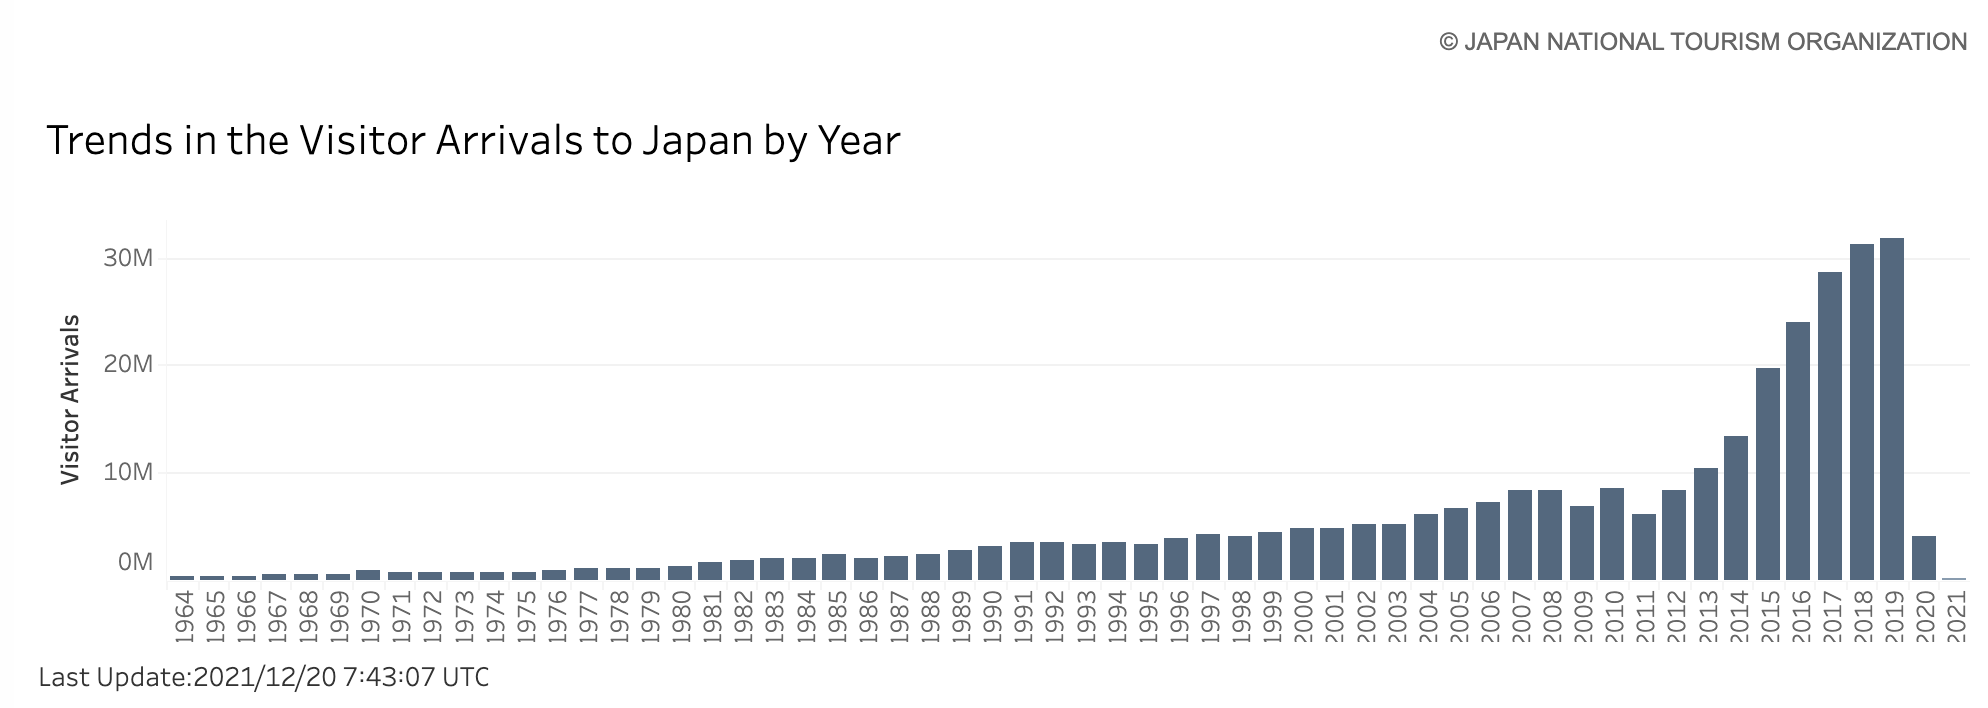
\includegraphics[width=\linewidth]{Figure/Figure1.png}
  \centering
  \caption[Foreign visitors number in Japan by year.]{Foreign visitors number in Japan by year.\protect\footnotemark }
  \label{fig1}
\end{figure*}
\footnotetext{https://statistics.jnto.go.jp/en/graph/\#graph--inbound--travelers--transition}
%\fi

After the 2018 Hokkaido Eastern Iburi earthquake, Survey Research Center, Inc. conducted a survey~\footnote{https://www.surece.co.jp/wp\_surece/wp-content/uploads/2018/09/20180914\_Result.pdf} on the evacuation behavior of foreign visitors to Japan. Survey Research Center, Inc. completed this survey in collaboration with JTB Corporation. The survey was completed on September 8th (Saturday) and 9th (Sunday), 2018. The survey chose the Hokkaido Tourism Information Center on Tanukikoji Shopping Street as the survey spot, and interviews were conducted by foreign-language speaking surveyors using the survey questionnaire. The survey collected 185 valid samples from foreign tourists visiting Japan who stayed in Hokkaido on September 6, 2018, asking about their behavior during the earthquake, evacuation guidance provided by accommodation facilities, and problems encountered during the earthquake. Mainland China, Taiwan, Hong Kong, the United States, and South Korea accounted for 70\% of the respondents' nationalities. The study's findings reveal a number of significant findings, including difficulties in earthquakes, behaviors have taken after the disaster happened, and desired response in the event of an earthquake.

First, the survey result of difficulties encountered by foreign visitors during the earthquake was shown in Figure~\ref{fig2a}. The inability to access information due to power outages and the inability to charge cell phones were the top-ranked difficulties. The third most difficult problem was a lack of supplies in supermarkets and convenience stores. The fourth-ranked difficulty was the schedule change caused by the earthquake. The fifth concern was not knowing where to go or what to do because of a language barrier. Lack of food/water supplies, uncertainty about the next trip, inability to understand earthquake information shown on TV, lack of information provided by transportation agencies/airports, and lack of earthquake evacuation manuals for foreigners that make it difficult to know what to do were the sixth to tenth-ranked difficulties. The lack of multilingual disaster/transportation/evacuation information in cell phones, the lack of evacuation instructions in hotels, the lack of information about the earthquake in Japan, the lack of information about what to bring to evacuate, and the lack of information from medical institutions were the eleventh to fifteenth difficulties. According to the results, the most common difficulties during the earthquake, were related to power outages, such as 'power outages made it difficult to get information' and 'power outages made it difficult to charge smartphones, etc' ( 67.0\%). Due to unforeseen circumstances caused by the earthquake, the response of 'lack of supplies at convenience stores and supermarkets'  (46.5\%) was also common. Respondents were concerned about modifications to their itinerary as a result of transportation disruptions, such as 'all my itineraries were disrupted and I had to pay a lot of money' (37.3\%) and 'I couldn't predict what would happen to my itinerary in the future'(27.0\%). Another common difficulty was related to language issues like 'I didn't know where to go because I didn't understand the language' (29.2\%).

Second, Figure~\ref{fig2b} shows the survey results of behaviors that occurred after the earthquake. Following the earthquake, the top three common actions were 'tried to get information via the Internet or SNS' (49.7\%), 'stayed where they were and checked on the situation' (44.3\%), and 'kept in touch with family and friends via the Internet, e-mail, and SNS such as Facebook and Line' (39.5\%). Calling family/friends (31.9\%), getting information about the earthquake from TV or radio (31.4\%), contacting the hotel front desk (27\%), and contacting fellow travelers (20\%) was the fourth to seventh popular responses. So, based on the survey results, we can conclude that after the earthquake, people prefer to stay in the area to look into the matter while gathering information and confirming their safety via the Internet and social media. In particular, we can discover that there are two main ways for respondents to gather information. The first is face-to-face information-seeking behaviors, such as asking people around, hotel staff, and so on. The other type of information-seeking behavior is no-face-to-face information-seeking behaviors. The other is no-face-to-face information-seeking behaviors, which primarily rely on television/radio/social media/internet. We will also divide people's information-seeking behaviors into these two types in the follow-up study to see whether people's behavioral patterns are more inclined to contact people or not.

%%%%%%%%%%%%%%%%%%%%%%%%%%%%%%%%
%\iffalse
\begin{figure*}[h]
  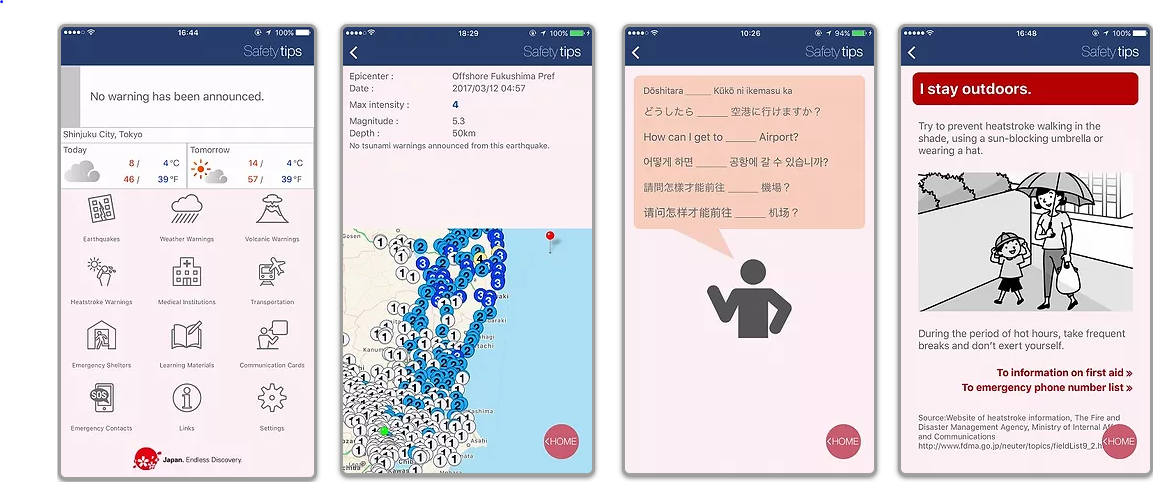
\includegraphics[width=\linewidth]{Figure/Figure3.png}
  \centering
  \caption[Safety Tips' interface]{Safety Tips' interface.\protect\footnotemark }
  \label{fig3}
\end{figure*}
\footnotetext{https://www.rcsc.co.jp/safety}

\begin{figure*}[h]
  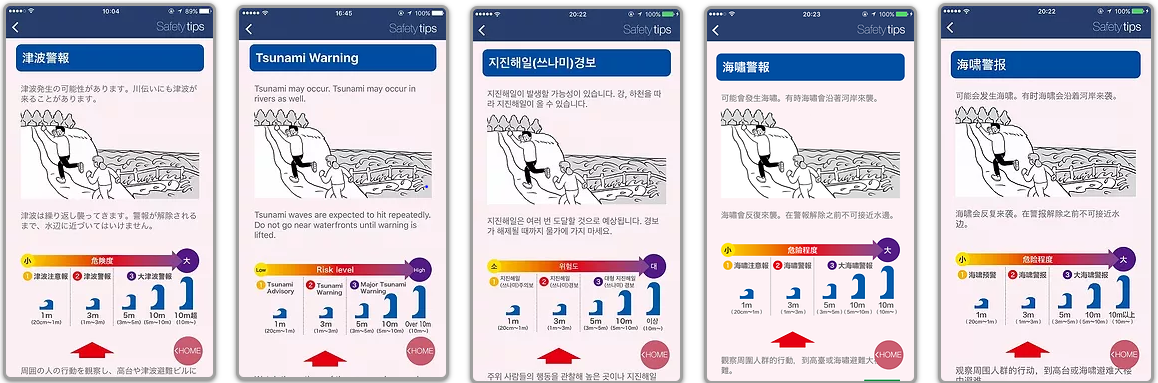
\includegraphics[width=\linewidth]{Figure/Figure4.png}
  \centering
  \caption[Multilingual Notifications for Safety Tips]{Multilingual Notifications for Safety Tips\protect\footnotemark }
  \label{fig4}
\end{figure*}
\footnotetext{https://www.rcsc.co.jp/safety}
%\fi

Third, as shown in Figure~\ref{fig2c}, popular desired responses in the event of an earthquake were 'Provide charging points, etc.' (50.8\%) and 'Enhance information centers' (42.2\%), followed by 'Distribute manuals in native languages' (38.4\%). And the next most common responses can be roughly divided into three categories. The first is a requirement for multilingual services, such as 'want evacuation guidance in a language I understand' (36.2\%) or 'want disaster/traffic/evacuation information to be provided in multiple languages via smart phones, etc.' (35.1\%), 'Would like TVs and other media to display information in English' (30.8\%), 'Would like information signs in my native language' (24.9\%). Another requirement was for a place of evacuation, such as 'providing places to stay and other accommodations'(34.6\%), 'Would like the hotel where I was staying to serve as a disaster information hub' (22.2\%). The last category was for providing information, such as 'Would like information centers to be set up to provide information on transportation and flights' (25.4\%), 'Provide telephone consultation services'(15.1\%), and 'Would like pamphlets and other materials that show what to do after an evacuation'(14.1\%), and 'Wish to learn more about medical institutions' (9.2\%).

Combined with the previous findings in the survey, it is clear that there is a need to provide sufficient places for foreign visitors to recharge in order to ensure that they can contact their family/friends and gather the necessary disaster information from social media/networks. The following step is to provide information in their language as well as evacuation assistance.

Considering the Japan Tourism Agency has constantly concern with issues of security and safety in the tourism industry. So, under the supervision of the Japan Tourism Agency, R.C. Solutions, Inc. developed a free application called Safety tips, which can notify foreign visitors of earthquake early warnings, tsunami warnings, eruption alerts, special warnings, heatstroke information, national protection information, evacuation advisories, and other disasters that occurred in Japan. Figure~\ref{fig3} shows the Safety Tips interface. During disasters, safety tips can provide a variety of purposes for foreign visitors to Japan. It is available in 14 languages (15 languages), including Japanese, English, Chinese (traditional and simplified), Korean, Spanish, Portuguese, Vietnamese, Thai, Indonesian, Tagalog, Nepali, Khmer, Burmese, and Mongolian (as shown in Figure~\ref{fig4}). Safety Tips is an important part of this study. The study will compare the difference in attitudes toward Safety Tips among respondents of various nationalities, as well as the differences in attitudes toward Safety Tips among people from various upbringing backgrounds.

%%%%%%%%%%%%%%%%%%%%%%%%%%%%
%\iffalse
\begin{figure*}[h]
  \begin{subfigure}{\textwidth}
    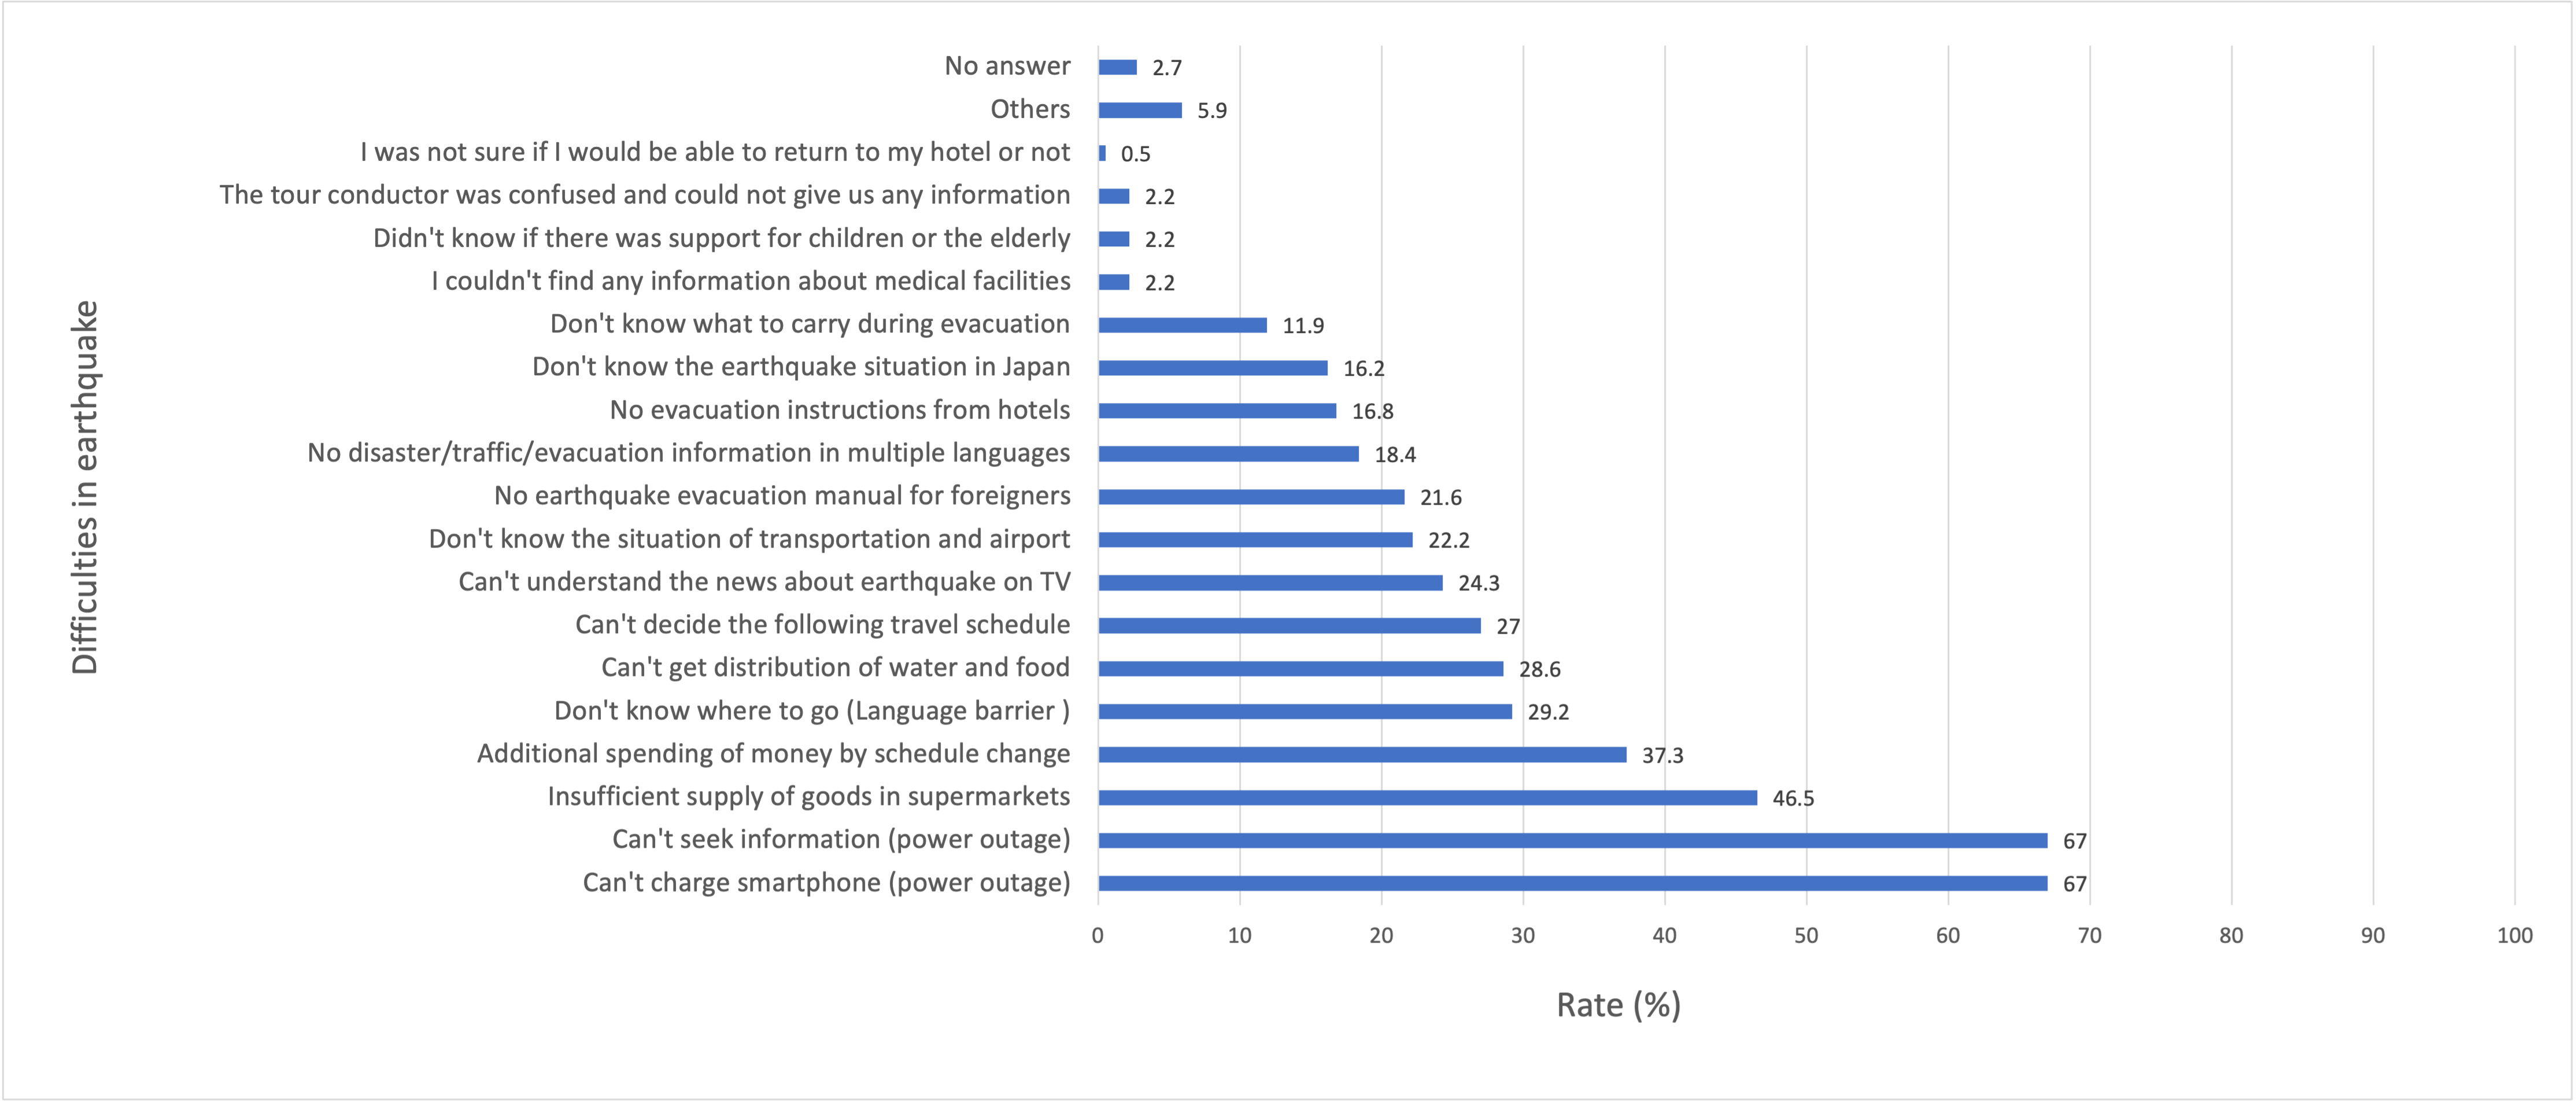
\includegraphics[width=\linewidth]{Figure/Figure2a.png}
    \caption{Difficulties in earthquake}
    \label{fig2a}
  \end{subfigure}
  \begin{subfigure}{\textwidth}
    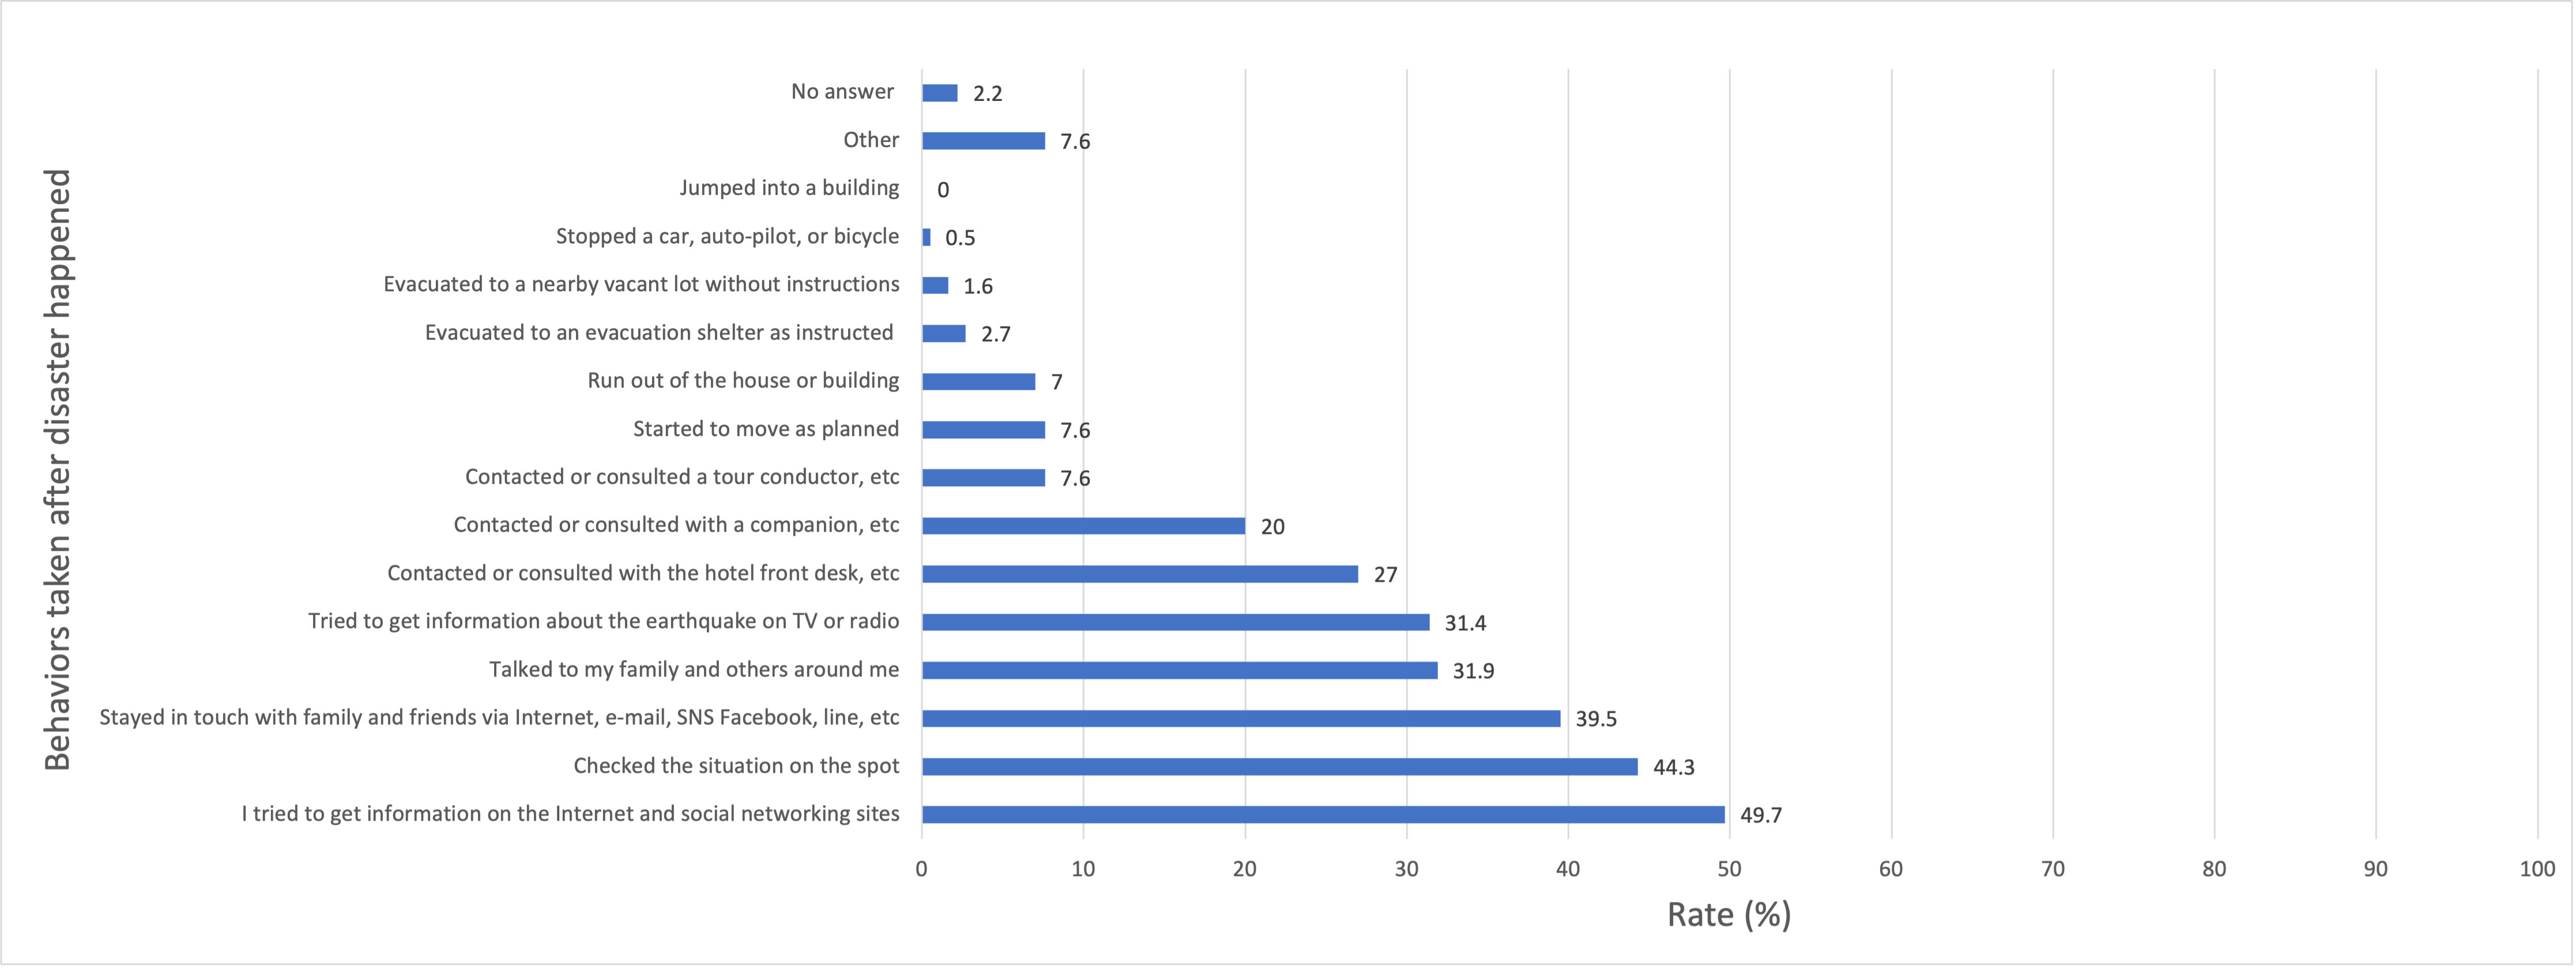
\includegraphics[width=\linewidth]{Figure/Figure2b.png}
    \caption{Behaviors taken after the disaster happened}
    \label{fig2b}
  \end{subfigure}
  \begin{subfigure}{\textwidth}
    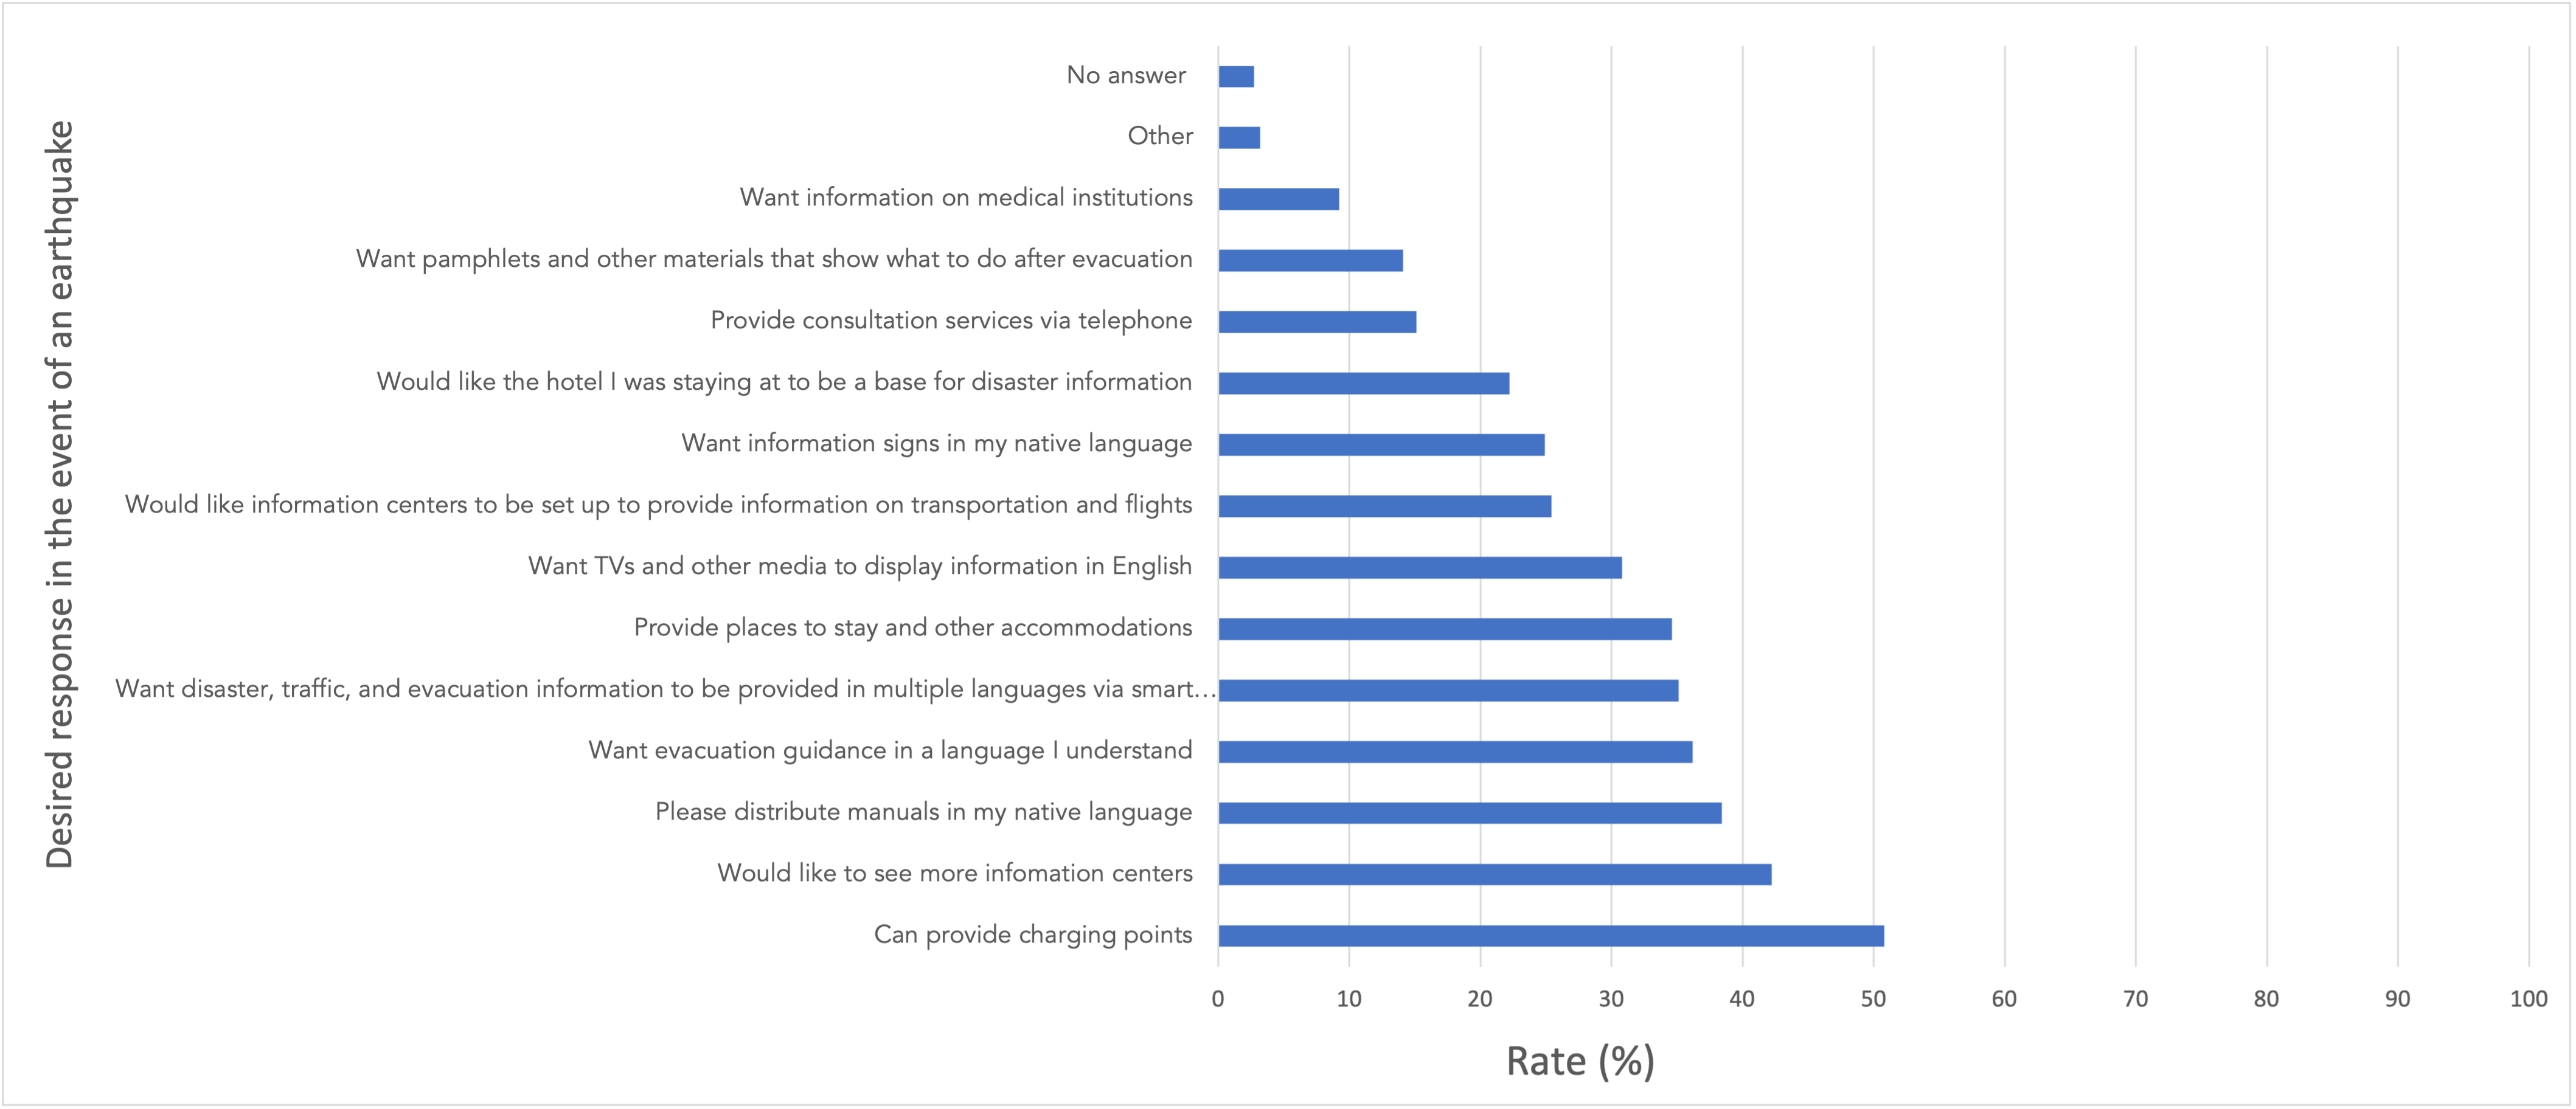
\includegraphics[width=\linewidth]{Figure/Figure2c.png}
    \caption{Desired response in the event of an earthquake}
    \label{fig2c}
  \end{subfigure}
  \centering
  \caption[Survey on Evacuation Behavior of foreign visitors to Japan after the 2018 Hokkaido Eastern Iburi earthquake.]{Survey on Evacuation Behavior of foreign visitors to Japan after the 2018 Hokkaido Eastern Iburi earthquake.\protect\footnotemark }
  \label{fig2}
\end{figure*}
\footnotetext{https://www.surece.co.jp/research/2491/}
%\fi
\cleardoublepage

\section{Problem Identification}
Based on the above, we can understand that foreign visitors will face numerous challenges when a disaster strikes while visiting. Because earthquakes and other natural disasters are relatively common in Japan, Japanese children learn about evacuation at a young age and participate in numerous evacuation/evacuation drills and exercises. However, there would be many differences between Japanese and foreign visitors. For example, for foreign visitors, it is unknown whether they have previously experienced disasters, whether they learned about evacuation as children, or whether they have participated in earthquake simulation drills. As a result, they would behave differently with the Japanese during the evacuation. Therefore, it is important to explore the behavioral differences between foreign visitors and Japanese. The results of a questionnaire survey were analyzed in this study to explore the patterns of evacuation behavior preferred by foreign visitors, as well as the differences between Japanese and foreign visitors.

Furthermore, to make Safety Tips more useful to foreign visitors, we first should understand their attitudes toward the use of Safety Tips. As a result, the first section of this study will explore the difference in attitudes toward Safety Tips among foreign visitors from various countries. Second, we will explore whether their prior use of Safety Tips influences their subsequent attitudes toward Safety Tips. In addition, structural equation modeling will be used in this order to examine how some personal characteristics influence respondents' attitudes toward Safety Tips. The personal characteristics include nationality, age, travel experience, disaster prevention education level, language ability, disaster experience, disaster prevention consciousness. These are discussed in depth in Chapter~\ref{c3}.

\section{Research Goal and Objective}
The goal of this study is to clarify the information-seeking and evacuation behavior of foreign visitors to Japan, as well as their perception of Safety Tips. 

This study has three main research objectives. The first objective is to understand foreign visitors' attitudes toward Safety Tips. The second objective is to explore how respondents' attitudes toward Safety Tips are influenced by their characteristics. The third objective is to explore the patterns of information seeking and evacuation behaviors, including which behavior comes first after the disaster happens and which behavior was used more frequently during the disaster. Finally, based on the findings of the research, provide improvement suggestions to Safety Tips.


\section{Thesis Structure}
This thesis begins with the first chapter, introduction, which explains the study's background, research questions, objectives and goals, and thesis structure. The introduction chapter's purpose is to provide background for the entire study and to help the reader in understanding the research topic. Then, the second chapter of the thesis focuses on the literature review. Considering that in this study, it is necessary to make the basic hypothesizes of Structural Equation Modeling based on prior research, so Chapter~\ref{c2} reviews some relevant studies in the field of evacuation research and establishes the basic hypothesizes of relationships between factors like demographic information, educational background, past disaster experience, and disaster training experience. The interpretation of the survey and data used in this study are presented in Chapter~\ref{c3}. Because the data in this study is extensive and complex, I intend to provide a more complete description in Chapter~\ref{c3} to help the reader understand it better. Chapter~\ref{c4} is about methodology, which includes the introduction and academic explanation of each methodology used to achieve each of the research objectives. Next, Chapter~\ref{c5} is results and analysis. Since this research is based on the analysis of data to clarify foreign visitors' behaviors and make suggestions of Safety Tips, this chapter shows and analyzes the results of the model one by one. The final chapter, Chapter~\ref{c6}, is the conclusion section. This chapter contains a summary conclusion of the whole study, some suggestions based on the results to help Safety Tips for better development, and the limitations in this study.


%% Some LaTeX commands I define for my own nomenclature.
% If you have to, it's better to change nomenclature once here than in a 
% million places throughout your thesis!


%======================================================================
\chapter{Literature Review}
\label{c2}
%======================================================================

As people's awareness of disaster prevention has increased in recent years, the number of disaster prevention and evacuation studies has increased year after year. On the other hand, using statistical knowledge to analyze some sociological issues is also one of the popular research directions. This research is a hybrid of the two domains mentioned above. This study focuses on people's evacuation behavior in terms of disasters, to promote a link between the respondents' demographic information elements, prior experiences with travel/evacuation dramas/disasters, and their behavior patterns in disasters. On the other side, the researchers measured how the above characteristics influenced their perceptions of the disaster prevention application called Safety Tips. Therefore, the analysis methods of many sociology-oriented studies for questionnaires, especially those containing scale-based questions, were also referred to. The following are the primary papers cited in this study.
\begin{itemize}
  \item A Study on the Dissemination Way of Disaster Information to Foreign Tourists to Japan~\cite{ref8}. 
  \item Incorporating human factors in emergency evacuation – An overview of behavioral factors and models~\cite{ref9}.
  \item Impact of ride-hailing apps on traditional LAMAT services in Asian developing cities: The Phnom Penh Case~\cite{ref7}.
\end{itemize}

\section{A Study on the Dissemination Way of Disaster Information to Foreign Tourists to Japan}

This paper provides an overview of how visitors to Japan obtain information about natural disasters from tourist guides and other sources. Furthermore, it investigates how foreign visitors to Japan are effectively provided with information about natural disasters in Japan through the behavior of foreign tourists and the responses of government agencies and other administrative bodies during the 2016 Kumamoto earthquake and the 2018 Hokkaido earthquake.

While tourists can get some information on disaster preparedness from guidebooks and other sources, the paper mentions that foreign visitors who have never experienced a real earthquake in the past may feel anxious when a disaster occurs in an unfamiliar country. One point raised in the paper that had previously gone unnoticed was that, while the priority in a disaster is to prevent death or injury, the post-disaster care needs of foreign visitors differ from those of Japanese citizens. The most immediate post-disaster needs of most foreign visitors in the Kumamoto and Hokkaido earthquakes were a desire to leave the disaster area as soon as possible and an attempt to gather transportation information. This is also a revelation for this study, which is why the analysis was conducted in order to investigate the differences between Japanese and foreign visitors. Because of the differences in backgrounds, developing Safety Tips based on the habits and habits of Japanese people may not be effective in assisting foreign visitors. As a result of this thesis, we have made it a priority to investigate the differences in evacuation behavior between Japanese and foreign visitors.

In addition, the paper investigates how to provide timely and accurate information to foreign visitors to Japan in the immediate aftermath of a natural disaster, despite language barriers. The authors make three points: 1) it is critical to provide information to foreign visitors in the event of a disaster; 2) there is a need to propose a method that makes it easier to provide information to foreign visitors across language barriers; and 3) because foreign visitors' reactions to disasters are influenced by previous disaster experiences, there is a need to provide a detailed description of the disaster in the context of the visitors' own culture. Furthermore, because Japanese maps, kanji, addresses, and other symbols were difficult for foreign visitors to understand, it was difficult for foreign visitors to locate evacuation centers simply by translating the maps into English. Furthermore, even if they find a structure that appears to be an evacuation shelter, it is difficult for them to determine whether the structure is a safe place to evacuate. As a result, national languages and easily recognizable signs were required to indicate that the building was an "evacuation center." This would not only confirm that the shelter was open to foreigners but would also assist the Japanese in recognizing it as a location where foreigners could flee. These suggestions made by the authors are significant for the present study. This is because this study will eventually use the results of the analysis to make some recommendations that will be beneficial to the development of Safety Tips. Several of the ideas mentioned in the paper can be further refined to be reflected in Safety Tips in order to better assist foreign visitors.

\section{Incorporating human factors in emergency evacuation – An overview of behavioral factors and models}
This research focuses on the relationship between people's evacuation behaviors and a variety of factors. To establish the hypotheses used in this study, it is important to refer to the results of previous studies on the relationship between people's selected behavior in evacuation and various factors. Many previous papers have addressed the subject of whether and how various factors affect evacuation behavior in evacuation, as stated in this study. The authors of this thesis, however, state that while these studies cover a wide spectrum of threats and disasters as well as evacuee behavior, it lacks a general classification of the elements that influence evacuation behavior. As a result, the authors present a clearer framework in this research to describe how aspects related to evacuation interact. As a result, the authors present a clearer framework in this research that explains how factors related to evacuation behavior influence people's decision to evacuate. Personal, environmental, and intervention variables are the three types of factors. 

Individual factors were divided into two subcategories by the authors: static factors and social factors. In the disaster evacuation process, static factors are inherent and stable. Evacuation is closely related to socio-demographic factors like age, race, or gender, as well as socio-economic factors like education level or family characteristics. The paper also mentioned three other personal characteristics: hazard experience, knowledge, and ability/deficiency. Given that the questionnaire questions in this study included demographic factors such as age and gender, as well as individual factors such as hazardous experience, knowledge, and ability, I believe this paper is very useful in developing the hypotheses underlying this study. 

In addition to the above-mentioned individual factors, social characteristics are receiving increased attention due to their importance in shaping crowd behavior and group phenomena~\cite{ref10}. People are more likely to cooperate with others rather than act alone~\cite{ref11}, and situational altruism has been observed rather than mass panic~\cite{ref12}. This study mentions disaster awareness in Consciousness, which focuses on respondents' perceptions of disasters during the evacuation process, such as their sense of unease, Other-directed type, and Disastrous Imagination, among others. As a result, this component of the factors is also very useful in developing the hypothesis underlying this study. 
Sensory cues/external stimuli, hazard features, and built/engineered environment are the three categories of environmental factors. Sensory cues/external stimuli typically prompt evacuees to take specific actions during an evacuation, typically beginning with information-seeking behavior. The temporal and spatial characteristics of the hazard involved are referred to as hazard characteristics. Architectural/engineering environmental factors range from building layout and ancillary factors to area network configuration features. While this aspect of the factors will not be directly relevant to this study, this study needs to understand how external factors influence people's evacuation behavior and why people typically begin their evacuation with information-seeking behavior. Because Safety Tips is an information-provider application, it is advantageous that people need to search for information to develop Safety Tips. 
The final section introduces a new category of factors proposed by the assignment in this study, known as interventional factors. These are the elements that capture people's outside influences. This includes information and actions taken in response to a crisis, such as official information notification and guidance type actions. Although this part of the factors will not be directly related to this study, the available selections of information-seeking behaviors and evacuation behaviors in our questionnaire are related to official information and evacuation guidance, so this part is also useful in comprehending this study.

\section{Impact of ride-hailing apps on traditional LAMAT services in Asian developing cities: The Phnom Penh Case}

This paper explores the impact of ride-hailing apps (RHAs) on a traditional service like LAMAT drivers. As a case study, this paper analyzes survey data collected from 177 traditional auto-rickshaw drivers in Phnom Penh from December 11 to 14, 2018. By examining the proportional difference in their operational service before and after the development of RHAs, this study investigates the influence of RHAs on the operational service of Remork drivers who did not adopt RHAs. The proportional difference is determined as (Mean2-Mean1)/Mean1, and a negative value shows that Mean2 is decreasing proportionally in comparison to Mean1. The results of paired t-tests were also used to see if all of the variables were substantially different. 

This study also used structural equation modeling to see if the effects listed above would encourage drivers to use ride-hailing applications (RHAs). The study's underlying premise was developed by a previous investigation, and five hypotheses were to be investigated in the SEM. H1 hypothesis stated that RHA Impacts have a favorable influence on RHA Intention. The H2 hypothesis was that Appreciation of RHAs has a positive effect on Intention to Use RHAs. H3 hypothesis stated that RHA Appreciation has a favorable impact on RHA Impacts. H4 hypothesis was that Appreciation of RHAs has a positive effect on Government Support RHAs. H5 hypothesis is that government support for RHAs has a beneficial impact on RHA use intentions. In this study, the author assessed the SEM's goodness of fit by multiple indices: $\chi^2$, the Root Mean Square Error of Approximation (RMSEA), the Goodness-of-Fit Index (GFI), Adjusted GFI (AGFI), TuckerLewis Index (TLI), and Comparative Fit Index (CFI). The results of the study showed that RHAs had an impact on the operational services of Remork drivers who did not use RHAs. Because of the presence of RHA, their daily trips decreased by 47.7\%, their daily trip customers increased by 47.6\%, and their monthly revenue increased by 43.2\% ($p<0.01$). It was further found that traditional Remork drivers had no intention of adopting RHAs, despite the impact of their operational services by the emergence of RHAs. The results show that they are not interested in working with RHAs because they expect lower revenues. In addition, they did not show much interest in RHA given the lack of financial capacity to upgrade their vehicles and the fact that they already had potential customers. My study mainly refers to the application of Structural Equation Modeling and the research procedures of this paper.



%% Some LaTeX commands I define for my own nomenclature.
% If you have to, it's better to change nomenclature once here than in a 
% million places throughout your thesis!


%======================================================================
\chapter{Survey and Data}
%======================================================================
\label{c3}
\section{Survey Introduction}
This research is based on an Internet-based survey of Foreign visitors and Japanese who have visited Tokyo, conducted by the Economic and Social Research Institute. A total of 1800 people were surveyed, including 300 people from each country. The detailed information is shown in Table~\ref{table1}. 

%%%%%%%%%%%%%%%%%
%\iffalse
\begin{table}[h]
  \caption{Survey descriptions}
  \label{table1}
  \centering
  \begin{tabular}{|c|l|}
  \hline
  Respondent &  Foreign visitors and Japanese who have visited Tokyo \\
  \hline
  Nationality  &  China, Korea, Thailand, Indonesia, UK, Japan \\
  \hline
  Method       &  Internet-based web survey \\
  \hline
  \begin{tabular}{c}Items\end{tabular}          &  
\begin{tabular}{c}
\begin{minipage}[t]{0.76\textwidth}
  \begin{itemize}
      \setlength{\itemsep}{-0.1cm} 
      \item[\textbf{1.}]  Demographics  
      \item[\textbf{2.}]  Disaster prevention consciousness 
      \item[\textbf{3.}]  Disaster response education, experience on earthquakes
      \item[\textbf{4.}]  Knowledge and perception on earthquakes 
      \item[\textbf{5.}]  Information seeking and evacuation behavior in scenarios
      \item[\textbf{6.}]  Perception on Safety Tips
   \end{itemize} 
\end{minipage}
\end{tabular}\\
   \hline
   Samples   &  300 samples/country (Total: 1,800) \\ 
   \hline
   Survey period &  2019/9/2 to 2019/9/10.\\
   \hline
  \end{tabular}
\end{table}
%\fi

\section{Question description}
The survey was divided into 6 items, the detailed description and available answers of each question in \crefrange{table2item1}{table2item6}. 
The first item, FQ1-FQ7, consists of seven demographic questions, including nationality, gender, age, travel experience, and Japanese proficiency. The second to fourth items are Q1-Q10, which includes disaster consciousness, disaster training experience, earthquake experience, earthquake knowledge, and disaster response knowledge. The fifth item is Q11-Q14, which is about respondents' response actions in four scenarios during the "Tokyo Metropolitan Earthquake." ( I'll go over scenarios in 3.3). The sixth item is Q15-Q17, which is about respondents' attitudes toward Safety Tips, including respondents' usage experiences as well as their perceptions of Safety Tips.

%%%%%%%%%%%%%%%%%%%%%%%%
%\iffalse
\begin{table}[h]
  \caption[Questions descriptions of Item 1]{Questions descriptions of Item 1 (FQ1 to FQ7)}
  \label{table2item1}
  \centering
  \begin{tabular}{c|c|l}
    No.      & Question & \multicolumn{1}{|c}{Description}  \\
  \hline
    FQ1     & Country &  \begin{tabular}{l}Answer 1 to 6 as Japan, China, South Korea, Thailand,\\Indonesia, the UK \end{tabular} \\
  \hline
    FQ2     & Gender  &  \begin{tabular}{l}Answer 1 as Male, 2 as Female. \end{tabular} \\
  \hline
    FQ3     & Age &  \begin{tabular}{l}Answer 1 to 8 as age under 15, age 16-19, age 20-29, age\\30-39, age 40-49, age 50-59, age 60-69, age over 70. \end{tabular} \\
  \hline
    FQ4     & Visited Country &  \begin{tabular}{l}The total number of visits to the following countries/regions\\in the past year, including Japan, China Mainland, China\\Hong Kong, China Macau, Korea, Thailand, Malaysia,\\Singapore, Indonesia, India. The answer is presented as the\\total number of visits, or 0 if no visit was recorded. \end{tabular} \\
  \hline
    FQ5     & Visited Japan &  \begin{tabular}{l}The total number of visits to each city in Japan in the past\\year, including Hokkaido, Chiba, Tokyo, Yokohama, Nagoya,\\Kyoto, Osaka, Nara, Hakata, Okinawa. The answer is\\presented as the total number of visits and 0 for no visits. \end{tabular} \\
  \hline
    FQ6     & Visit Experience &  \begin{tabular}{l}This question asks for the number of visits to Tokyo (for\\Japanese) / Number of visits to Japan (for overseas).\\Answer 1 to 6 as 1 time, 2 times, 3 to 4 times, 5 to 6\\times, 7 to 9 times, over 10 times, and 0 for no visits. \end{tabular} \\
  \hline
    FQ7     &  Japanese Level &  \begin{tabular}{l}Answer 1 to 4 as Japanese Level: Cannot understand,\\Basic, Intermediate, Up Level. \end{tabular} \\
   \hline

  \end{tabular}
\end{table}

\begin{table}[h]
  \caption[Questions descriptions of Item 2]{Questions descriptions of Item 2 (Q1 to Q5): Answer based on the scale of 0 to 6, detailed as not at all applicable, mostly not applicable, somewhat not applicable, somewhat agree, mostly agree, strongly agree.)}
  \label{table2item2}
  \centering
  \begin{tabular}{c|l}
    No.      & \multicolumn{1}{|c}{Description}  \\
  \hline
    \textbf{Q1}       & \textbf{Disastrous Imagination} \\
  \hline  
    Q1\_1  & \begin{tabular}{l}Can imagine what people around me will do in the event of a disaster.\end{tabular} \\
    Q1\_2  & \begin{tabular}{l}Can imagine the supplies I will need in the event of a disaster.\end{tabular} \\
    Q1\_3  & \begin{tabular}{l}Can imagine what you would do in the event of a disaster.\end{tabular} \\
    Q1\_4  & \begin{tabular}{l}Can imagine what kind of damage the city would suffer in the event of\\a disaster.\end{tabular} \\
  \hline
    \textbf{Q2}       & \textbf{Sense of crisis} \\
  \hline
    Q2\_1  & \begin{tabular}{l}A disaster could happen tomorrow.\end{tabular} \\
    Q2\_2  & \begin{tabular}{l}Once a disaster strikes, I will be in trouble.\end{tabular} \\
    Q2\_3  & \begin{tabular}{l}It is difficult to reduce the damage caused by disasters through personal\\efforts alone.\end{tabular} \\
    Q2\_4  & \begin{tabular}{l}Disaster prevention should not be completed only in my own area, but\\also in cooperation with other areas. \end{tabular} \\
  \hline
    \textbf{Q3} & \textbf{Other-directed type} \\
  \hline
   Q3\_1   & \begin{tabular}{l}Like to communicate with others.\end{tabular} \\
   Q3\_2   & \begin{tabular}{l}Like places where people gather.\end{tabular} \\
   Q3\_3   & \begin{tabular}{l}Want to make many different kinds of friends.\end{tabular} \\
   Q3\_4   & \begin{tabular}{l}Want to do something for other people. \end{tabular}\\
  \hline
   \textbf{Q4} & \textbf{Anxiety} \\
  \hline
   Q4\_1  & \begin{tabular}{l}Often feel anxious.\end{tabular} \\
   Q4\_2  & \begin{tabular}{l}I think I am a worrier.\end{tabular} \\
   Q4\_3  & \begin{tabular}{l}When I start thinking about disasters, I fantasize about different patterns\\of damage.\end{tabular} \\
   Q4\_4  & \begin{tabular}{l}Always worried about the dangers around me.\end{tabular} \\
  \hline
   \textbf{Q5} & \textbf{Apathy about disasters} \\
  \hline
   Q5\_1  & \begin{tabular}{l}Don't want to do anything that is not in my best interest.\end{tabular} \\
   Q5\_2  & \begin{tabular}{l}Only think about things that are likely to happen in my immediate\\surroundings.\end{tabular} \\
   Q5\_3  & \begin{tabular}{l}Don't usually think about disasters.\end{tabular} \\
   Q5\_4  &  \begin{tabular}{l}Physical measures such as reinforcing earthquake-proof buildings and\\building breakwaters are enough to prevent disasters.\end{tabular} \\
   \hline

  \end{tabular}
\end{table}

\begin{table}[h]
  \caption[Questions descriptions of Item 3]{Questions descriptions of Item 3 (Q6 to Q8)}
  \label{table2item3}
  \centering
  \begin{tabular}{c|l}
    No.      & \multicolumn{1}{|c}{Description}  \\
  \hline
    \textbf{Q6} & \begin{tabular}{l}\textbf{Disaster training experience. (1 for yes, 0 for no)}\\\textbf{(12 questions for each of the 4 disasters include}\\\textbf{Q6\_1Earthquake, Q6\_2tsunami, Q6\_3typhoon, Q6\_4fire)}\end{tabular} \\
  \hline  
    (1)  & \begin{tabular}{l}Have you participated in drills (evacuation drills, disaster drills, etc.)?\end{tabular} \\
    (2)  & \begin{tabular}{l}Have received training at school or participated in a seminar.\end{tabular} \\
    (3)  & \begin{tabular}{l}Have received training at work or participated in a training session.\end{tabular} \\
    (4)  & \begin{tabular}{l}Have received training by the government or local government,\\or participated in a training session\end{tabular} \\
    (5)  & \begin{tabular}{l}Have received training or participated in training sessions by local\\community/community association, etc.\end{tabular} \\
    (6)  & \begin{tabular}{l}Have received education or participated in a training session by\\a private organization or group.\end{tabular} \\
    (7)  & \begin{tabular}{l}Have received training or participated in a workshop other than\\the above.\end{tabular} \\
    (8)  & \begin{tabular}{l}Have seen or heard disaster information on TV or radio programs.\end{tabular} \\
    (9)  & \begin{tabular}{l}I have seen disaster information in newspapers or magazines.\end{tabular} \\
    (10)  & \begin{tabular}{l}Have seen disaster information on bulletin boards, etc.\end{tabular} \\
    (11)  & \begin{tabular}{l}Have seen disaster information on the Internet (disaster\\prevention-related websites of government or public organizations)\end{tabular} \\
    (12)  & \begin{tabular}{l}Have you ever seen disaster information on the Internet (disaster-related\\websites of private organizations or local communities)?\end{tabular} \\
  \hline
    \textbf{Q7}       &  \begin{tabular}{l}\textbf{Number of disaster training (Answer 1 to 4 as one time,}\\\textbf{2 to 3 times, 4 to 6 times, over 7 times.)} \end{tabular} \\
  \hline
   Q7\_1   & \begin{tabular}{l}Earthquake\end{tabular} \\
   Q7\_2   & \begin{tabular}{l}Tsunami \end{tabular} \\
   Q7\_3   & \begin{tabular}{l}Typhoon\end{tabular} \\
   Q7\_4   & \begin{tabular}{l}Fire\end{tabular}\\
  \hline
   \textbf{Q8} & \begin{tabular}{l}\textbf{Earthquake experience (Q8 is about the severity of the}\\\textbf{earthquake experienced. Answer 1 to 8 as MMI intensity}\\\textbf{5 or less / intensity 3 or less; MMI intensity 6 / intensity}\\\textbf{4; MMI intensity 7 / intensity 5 weak; MMI intensity}\\\textbf{8 / intensity 5 strong; MMI intensity 9 / intensity 6 weak;}\\\textbf{MMI intensity 10 / intensity 6 strong; MMI intensity 11}\\\textbf{to 12 / intensity 7; no experience)}\end{tabular} \\
   \hline
  \end{tabular}
\end{table}

\begin{table}[h]
  \caption[Questions descriptions of Item 4]{Questions descriptions of Item 4 (Q9 and Q10): Answer based on the scale of 0 to 6, detailed as don't know anything about it, almost don't know, somewhat unfamiliar, somewhat familiar, know almost about it, know very much.}
  \label{table2item4}
  \centering
  \begin{tabular}{c|l}
    No.      & \multicolumn{1}{c}{Description}  \\
  \hline
    \textbf{Q9} & \textbf{Knowledge about earthquakes} \\
  \hline  
    (1)  & \begin{tabular}{l}Magnitude is the strength of the tremor and differs from place to place.\end{tabular} \\
    (2)  & \begin{tabular}{l}Magnitude is the size of an earthquake.\end{tabular} \\
    (3)  & \begin{tabular}{l}A small increase in magnitude can result in an unimaginably large\\earthquake.\end{tabular} \\
    (4)  & \begin{tabular}{l}The magnitude of an earthquake and the amount of damage caused by an\\earthquake are affected not only by the size of the earthquake but also by\\the distance from the epicenter and the characteristics of the ground.\end{tabular} \\
    (5)  & \begin{tabular}{l}The method of measurement is different between the Japanese seismic\\intensity and the global seismic intensity (Mercari seismic intensity scale).\end{tabular} \\
    (6)  & \begin{tabular}{l}In Japan, seismic intensity information is important when considering\\damage caused by earthquakes.\end{tabular} \\
  \hline
    \textbf{Q10}       & \textbf{Knowledge of how to respond to a disaster}  \\
  \hline
    (1)  & \begin{tabular}{l}Protect your head, move away from large furniture, and hide under a\\sturdy desk.\end{tabular} \\
    (2)  & \begin{tabular}{l}Do not run outdoors in a panic.\end{tabular} \\
    (3)  & \begin{tabular}{l}Open doors and windows to create an escape route.\end{tabular} \\
    (4)  & \begin{tabular}{l}Follow the instructions of the staff.\end{tabular} \\
    (5)  & \begin{tabular}{l}Do not rush to the exits or stairs.\end{tabular} \\
    (6)  & \begin{tabular}{l}Stop at the nearest floor and get off immediately.\end{tabular} \\
    (7)  & \begin{tabular}{l}Stay away from block walls, vending machines, buildings, etc.\end{tabular} \\
    (8)  & \begin{tabular}{l}Protect your head and move with caution to avoid falling signs, broken\\windows, etc.\end{tabular} \\
    (9)  & \begin{tabular}{l}Check your surroundings carefully and act calmly.\end{tabular} \\
   \hline
  \end{tabular}
\end{table}


\begin{table}[h]
  \caption[Questions descriptions of Item 6]{Questions descriptions of Item 6 (Q15 to Q17): About Safety Tips}
  \label{table2item6}
  \centering
  \begin{tabular}{c|l}
    No.      & \multicolumn{1}{|c}{Description}  \\
  \hline
     \        & \begin{tabular}{l}\textbf{Usage experience}\end{tabular}  \\
  \hline
   Q15      & \begin{tabular}{l}Do you know Safety tips or not? (Answer 1 to 3 as don't know, only heard\\the name before, know exactly.) (Answer 2 and 3 goes to Q16, Answer 1\\directly goes to Q17.)\end{tabular} \\
   Q16      & \begin{tabular}{l}Did you use Safety tips before or not? (Answer 1 is never used before, 2 is\\used before.) \end{tabular} \\
  \hline
   \textbf{Q17} &\begin{tabular}{l}\textbf{Attitude toward Safety Tips. (Answer based on the scale of 0 to 6,}\\\textbf{detailed as not at all applicable, mostly not applicable, somewhat}\\\textbf{not applicable, somewhat agree, mostly agree, strongly agree.)} \end{tabular}  \\
  \hline
   Q17\_1  & \begin{tabular}{l}Will you trust Safety tips more than information from your own country?\end{tabular} \\
   Q17\_2 & \begin{tabular}{l}Will you use Safety tips before searching for information from your own\\country?\end{tabular}\\
   Q17\_3  & \begin{tabular}{l}Do you think Safety tips could be useful during evacuation?\end{tabular} \\
   Q17\_4 & \begin{tabular}{l}Will you use Safety tips in the future?\end{tabular}\\
  \hline
  \end{tabular}
\end{table}
%\fi
\cleardoublepage

\section{Scenario description}
In item No.5, all respondents should answer their Information seeking and evacuation behavior in each of the following scenarios. There are two types of differences between the scenarios, resulting in four different scenarios. The first type of difference is network-related and is divided into "Telephone/internet is available" and "Telephone/internet is not available (A temporary power outage occurs)". The second type of difference is location-related, divided into "Staying in a tourist attraction" and "Moving by public transportation". Thus the 4 scenarios are shown in Table~\ref{table3}.


%%%%%%%%%%%%%%%%%%%%%
%\iffalse
\begin{table}[h]
  \caption{Scenarios descriptions}
  \label{table3}
  \centering
  \begin{tabular}{l|c|c}
               &  \begin{tabular}{c}  Staying in a\\tourist attraction \end{tabular} & \begin{tabular}{c}  Moving by public\\transportation \end{tabular}  \\
    \hline
    \begin{tabular}{c}Telephone / Internet is available\end{tabular}  & Scenario 1 & Scenario 3 \\
    \hline
    \begin{tabular}{c} Telephone / Internet is not available\\(A temporary power outage occurs)\end{tabular} & Scenario 2 & Scenario 4 \\
 
  \end{tabular}
\end{table}
%\fi


In order to answer response actions during the disaster, all respondents were requested to watch a simulation video of the "Tokyo Metropolitan Earthquake". The video is provided by the Cabinet Office,  and the simulation video has been translated into their native languages. The simulation video shows an earthquake of magnitude 7.3 that occurred in the southern part of Tokyo, happened on a winter evening in the year 20xx, and in order to show the damage, the landscape is represented brighter than it actually is. After watching the video, the respondents were requested to select 5 response actions with an order in each of the scenarios. Some screenshots of the simulation video are shown in Figure~\ref{fig5}.

In the pre-survey, we collected some common evacuation behaviors of foreign visitors and Japanese people. It's worth noting that selections 1-7 are only available in scenarios 1 and 3 because they require a phone/internet connection. Table~\ref{table4} contains a list of all selections as well as a detailed description of each one.

%%%%%%%%%%%%%%%%%%%%%
%\iffalse
\begin{table}[h]
  \caption{Available selections of Behaviors}
  \label{table4}
  \centering
  \begin{tabular}{c|l}
  \hline
  Selection & Actions - Information seeking behavior \\
  \hline
  1             & \begin{tabular}{l}Collect Information on the official websites of Japanese government agencies\\(Japan Meteorological Agency, National Police Agency, Fire and Disaster\\Management Agency, etc.)\end{tabular}\\
  2             & Collect Information with the disaster prevention app on your smartphone \\
  3             & Collect Information on news sites and disaster prevention portal sites \\
  4             & Collect Information on SNS (Twitter, Facebook, LINE, etc.) \\
  5             & Call the embassy of your country to collect Information \\
  6             & Collect Information from TV and radio \\
  7             & Check maps and digital signage to collect Information \\
  8             & Gather Information by calling out to Japanese people nearby \\
  9             & Contact staff at tourist Information centers to collect Information \\
  10           & Contact the hotel staff to collect Information \\
  11           & Contact public transport staff to collect Information \\
 \hline
 Selection & Actions - Evacuation behavior \\
 \hline
 12            & Stay at your current location \\
 13            & Secure necessary supplies (food, drinks, etc.) \\
 14            & Move to an open space, such as a nearby park \\
 15            & Move according to evacuation guidance \\
 16            & Move to the evacuation center on your own \\
 17            & Move in sync with the movements of people around you \\
 18            & Observe the surroundings because you don't know what to do \\
 \hline
 Selection  & Actions - others \\
 \hline
 19            & Others \\
 20            & Do nothing / Can do nothing \\
 21            & I don't know \\
 \hline
  \end{tabular}
\end{table}

\begin{figure*}[h]
  \begin{subfigure}{0.32\textwidth}
    \centering
    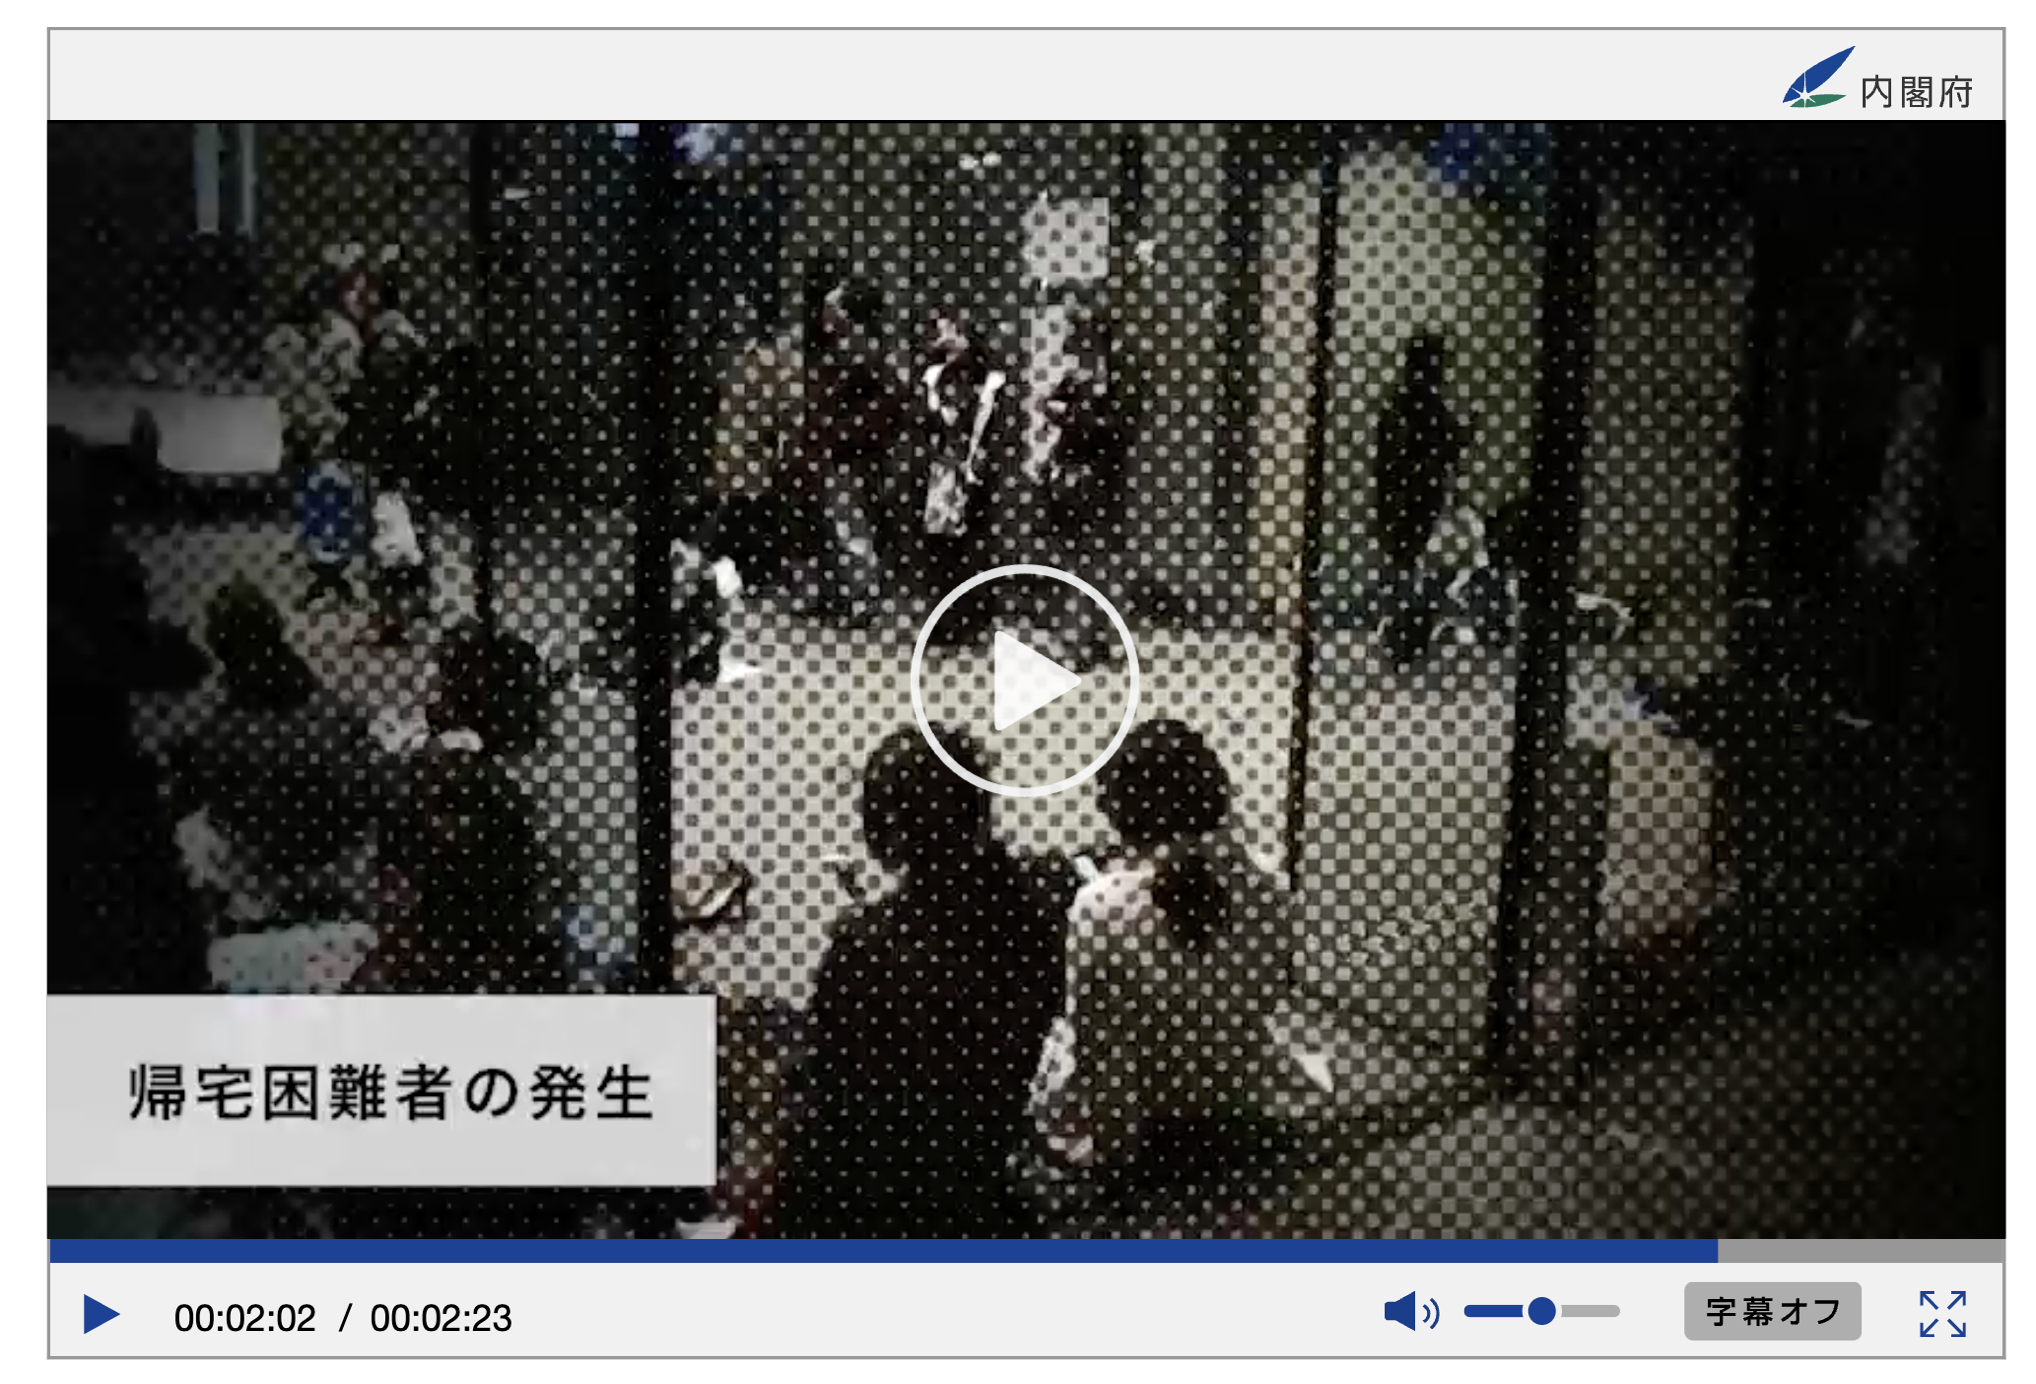
\includegraphics[width=\textwidth]{Figure/Figure5a.jpg}
    \caption{Difficulty in returning home}
    \label{fig5a}
  \end{subfigure}\hfill
  \begin{subfigure}{0.32\textwidth}
    \centering
    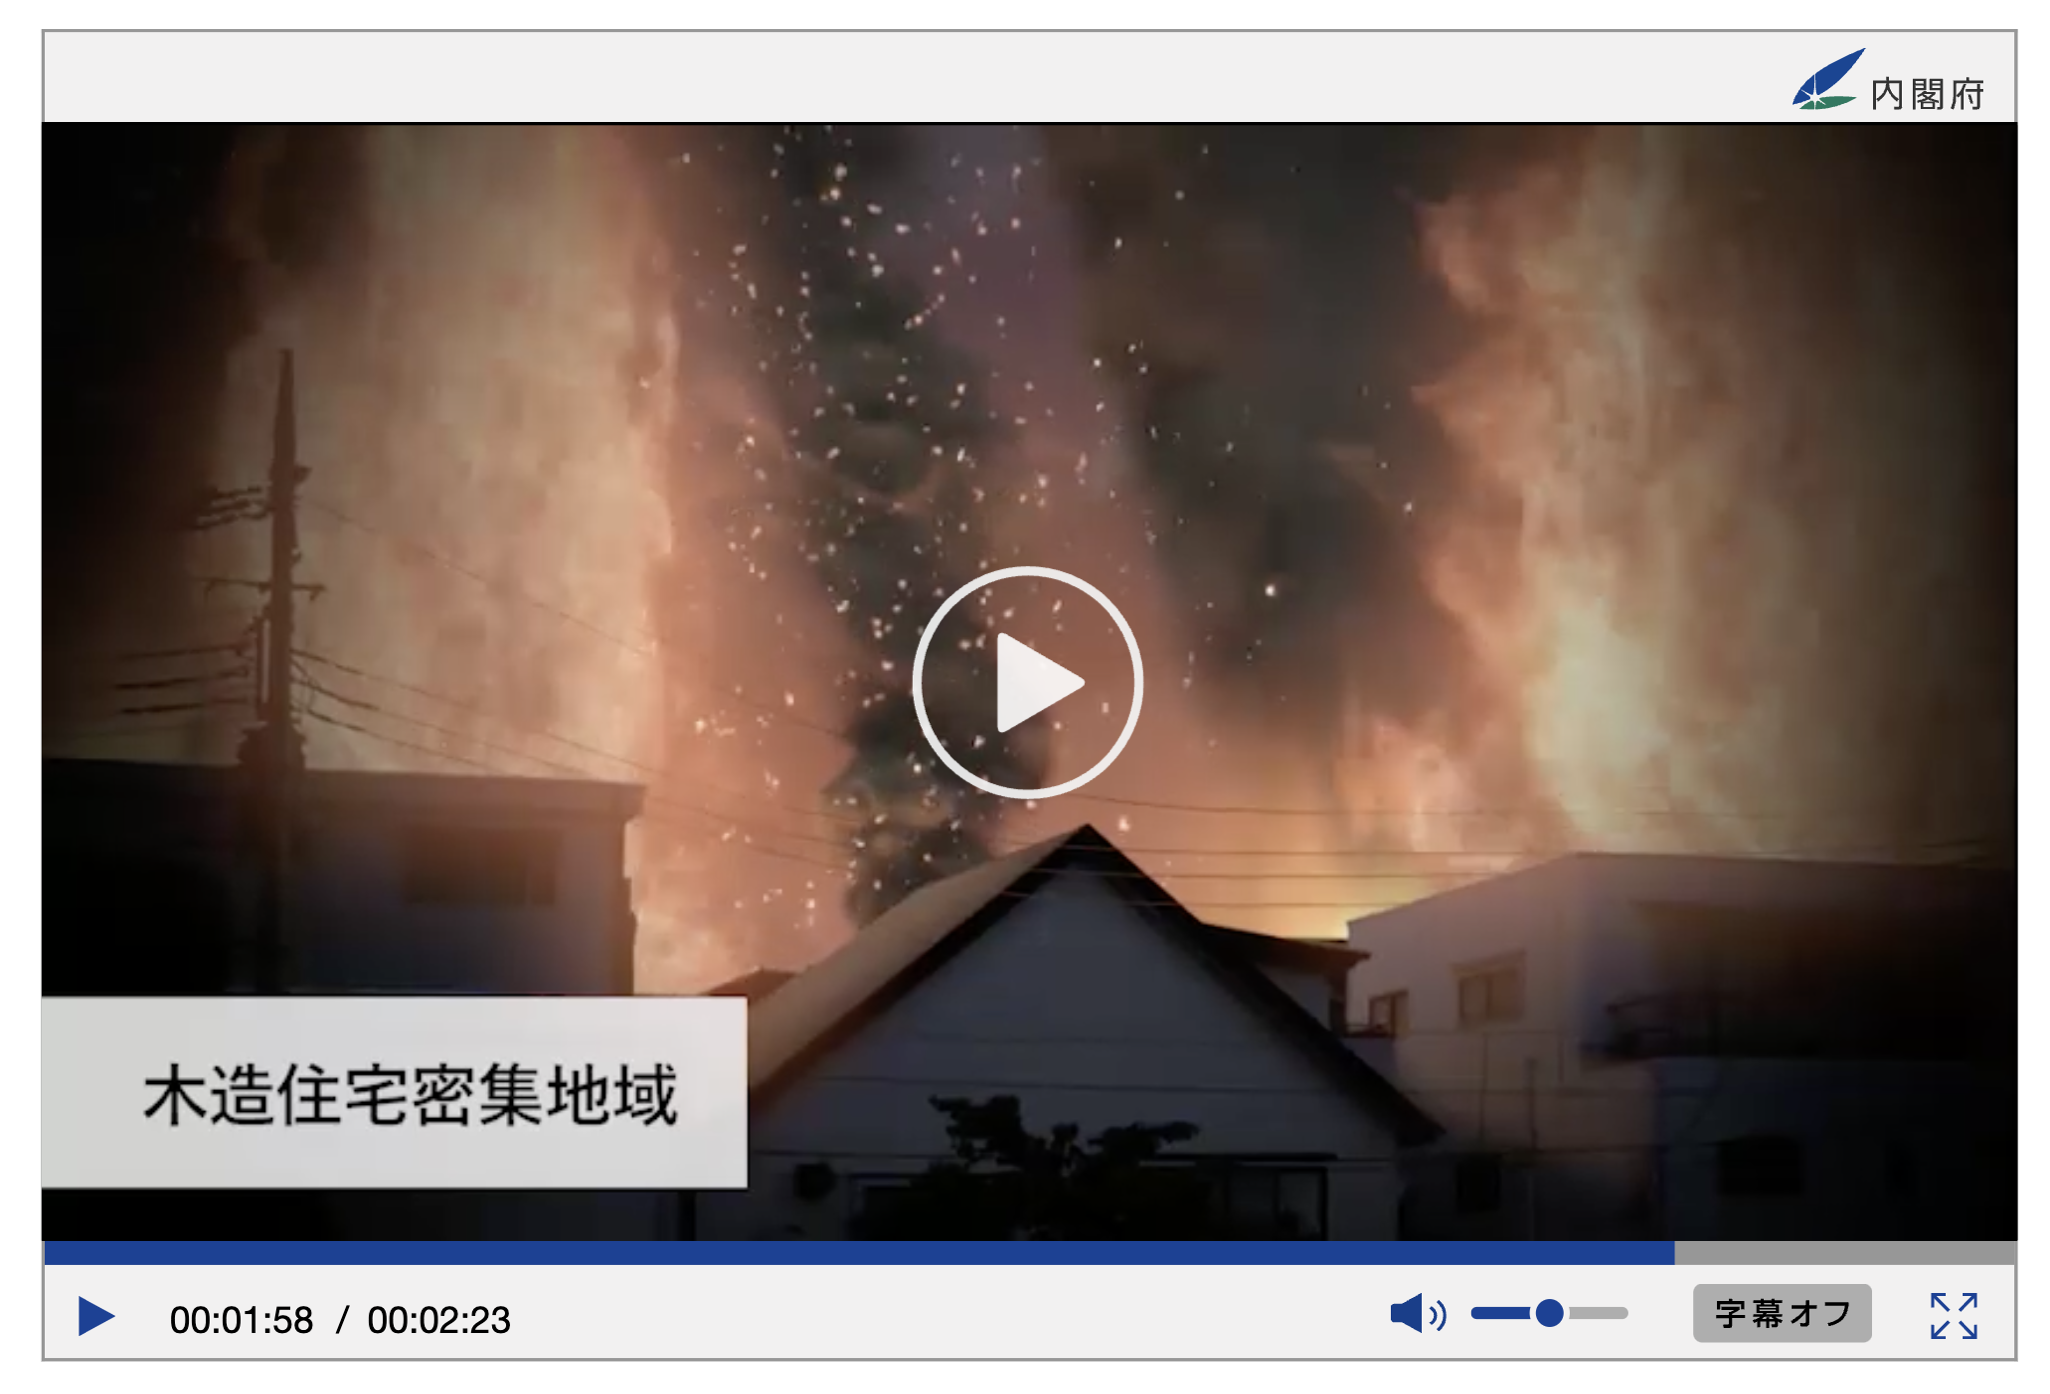
\includegraphics[width=\linewidth]{Figure/Figure5b.jpg}
    \caption{Dense area of wooden houses; Fire occurred easily}
    \label{fig5b}
  \end{subfigure}\hfill
  \begin{subfigure}{0.32\textwidth}
    \centering
    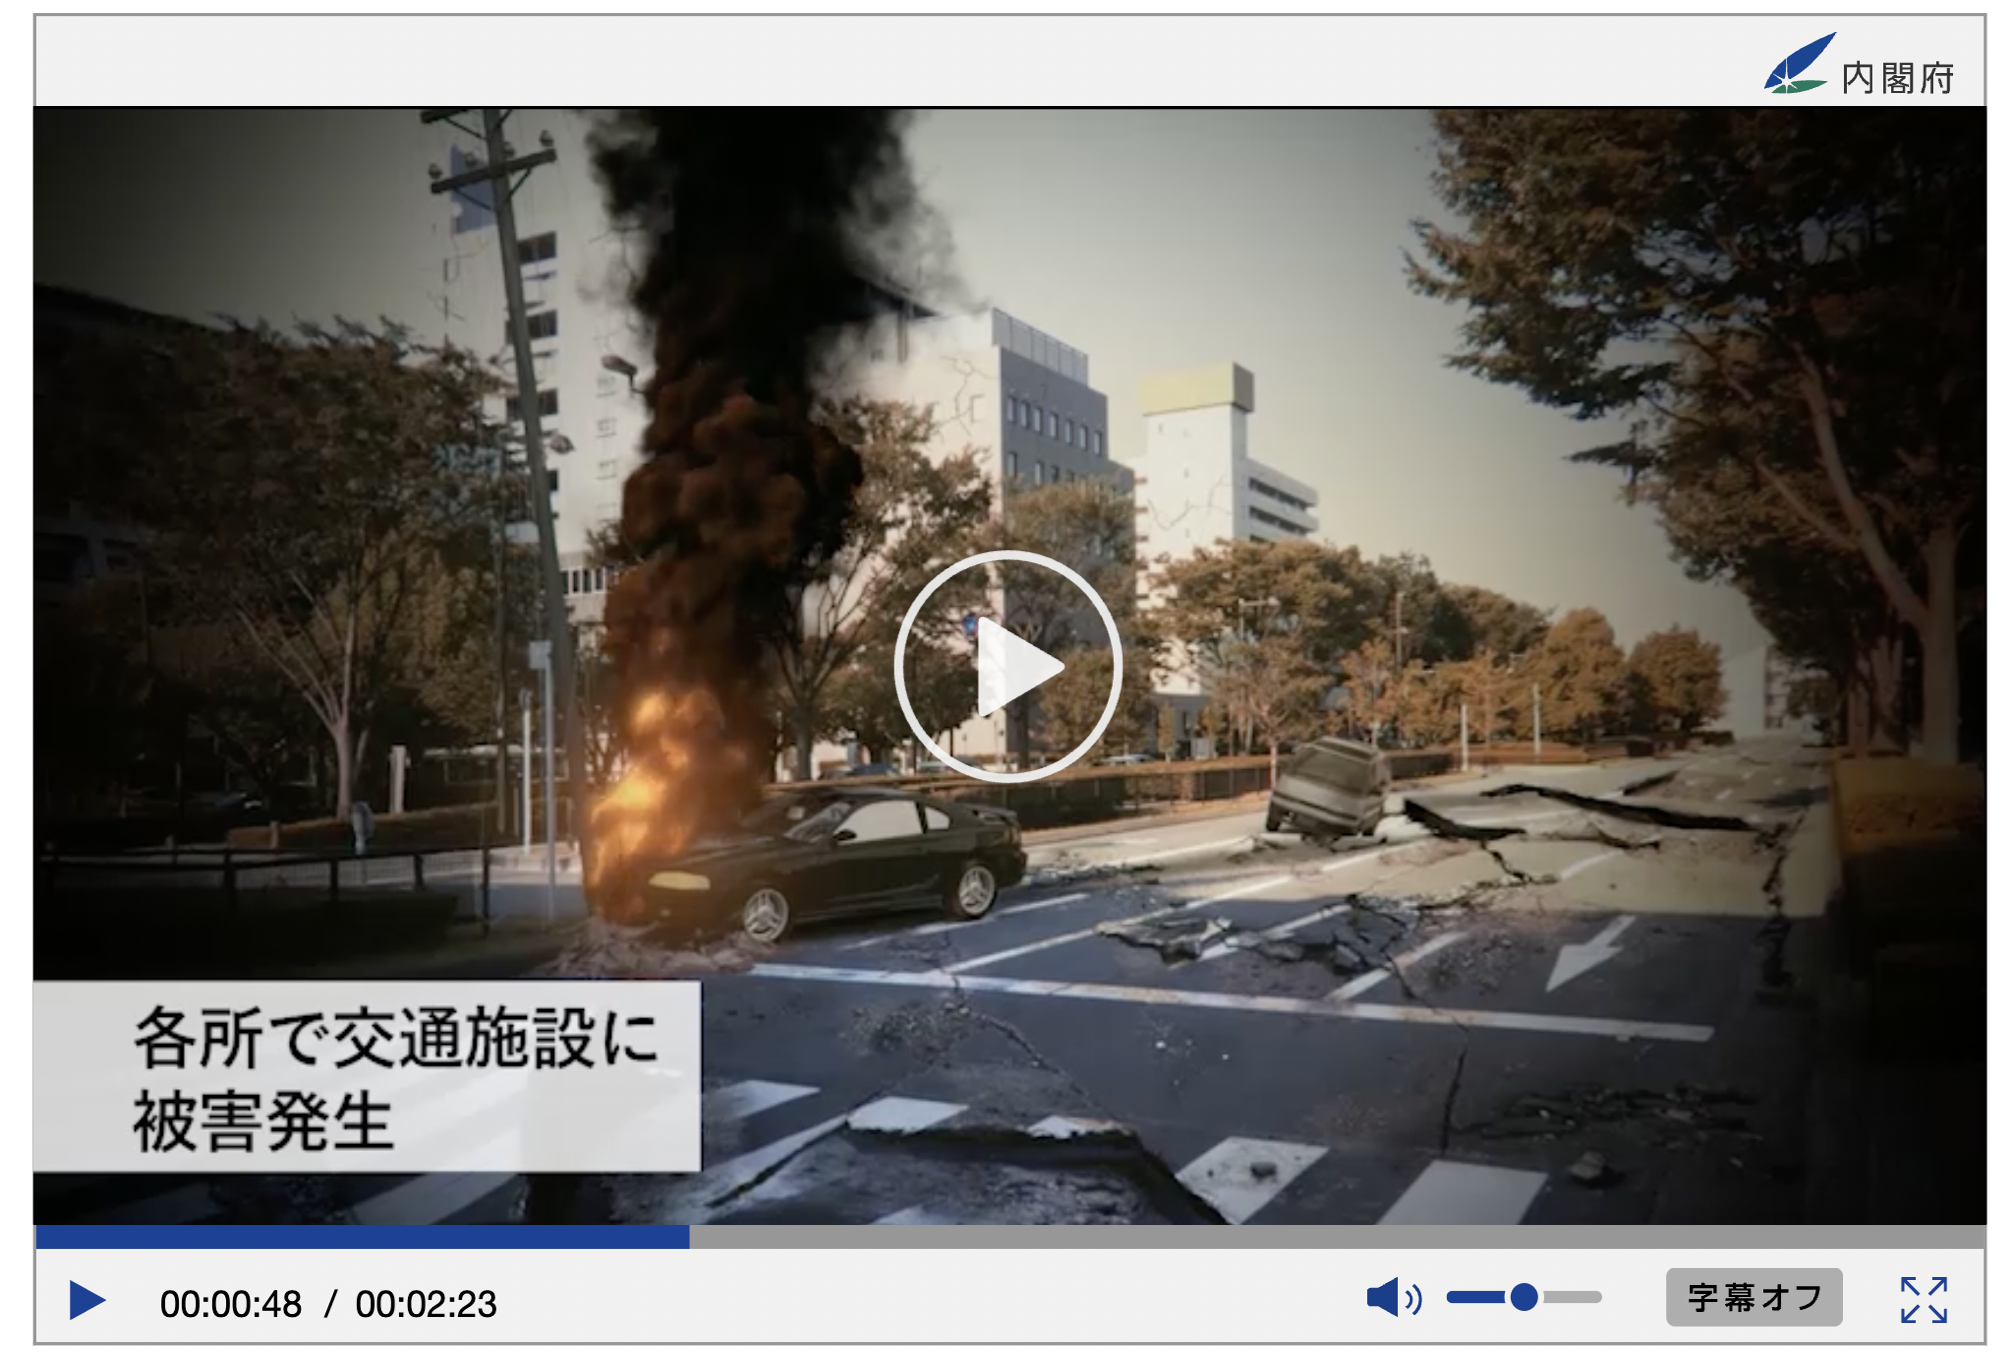
\includegraphics[width=\linewidth]{Figure/Figure5c.jpg}
    \caption{Damage to transportation facilities in many places}
    \label{fig5c}
  \end{subfigure}\hfill
  \begin{subfigure}{0.32\textwidth}
    \centering
    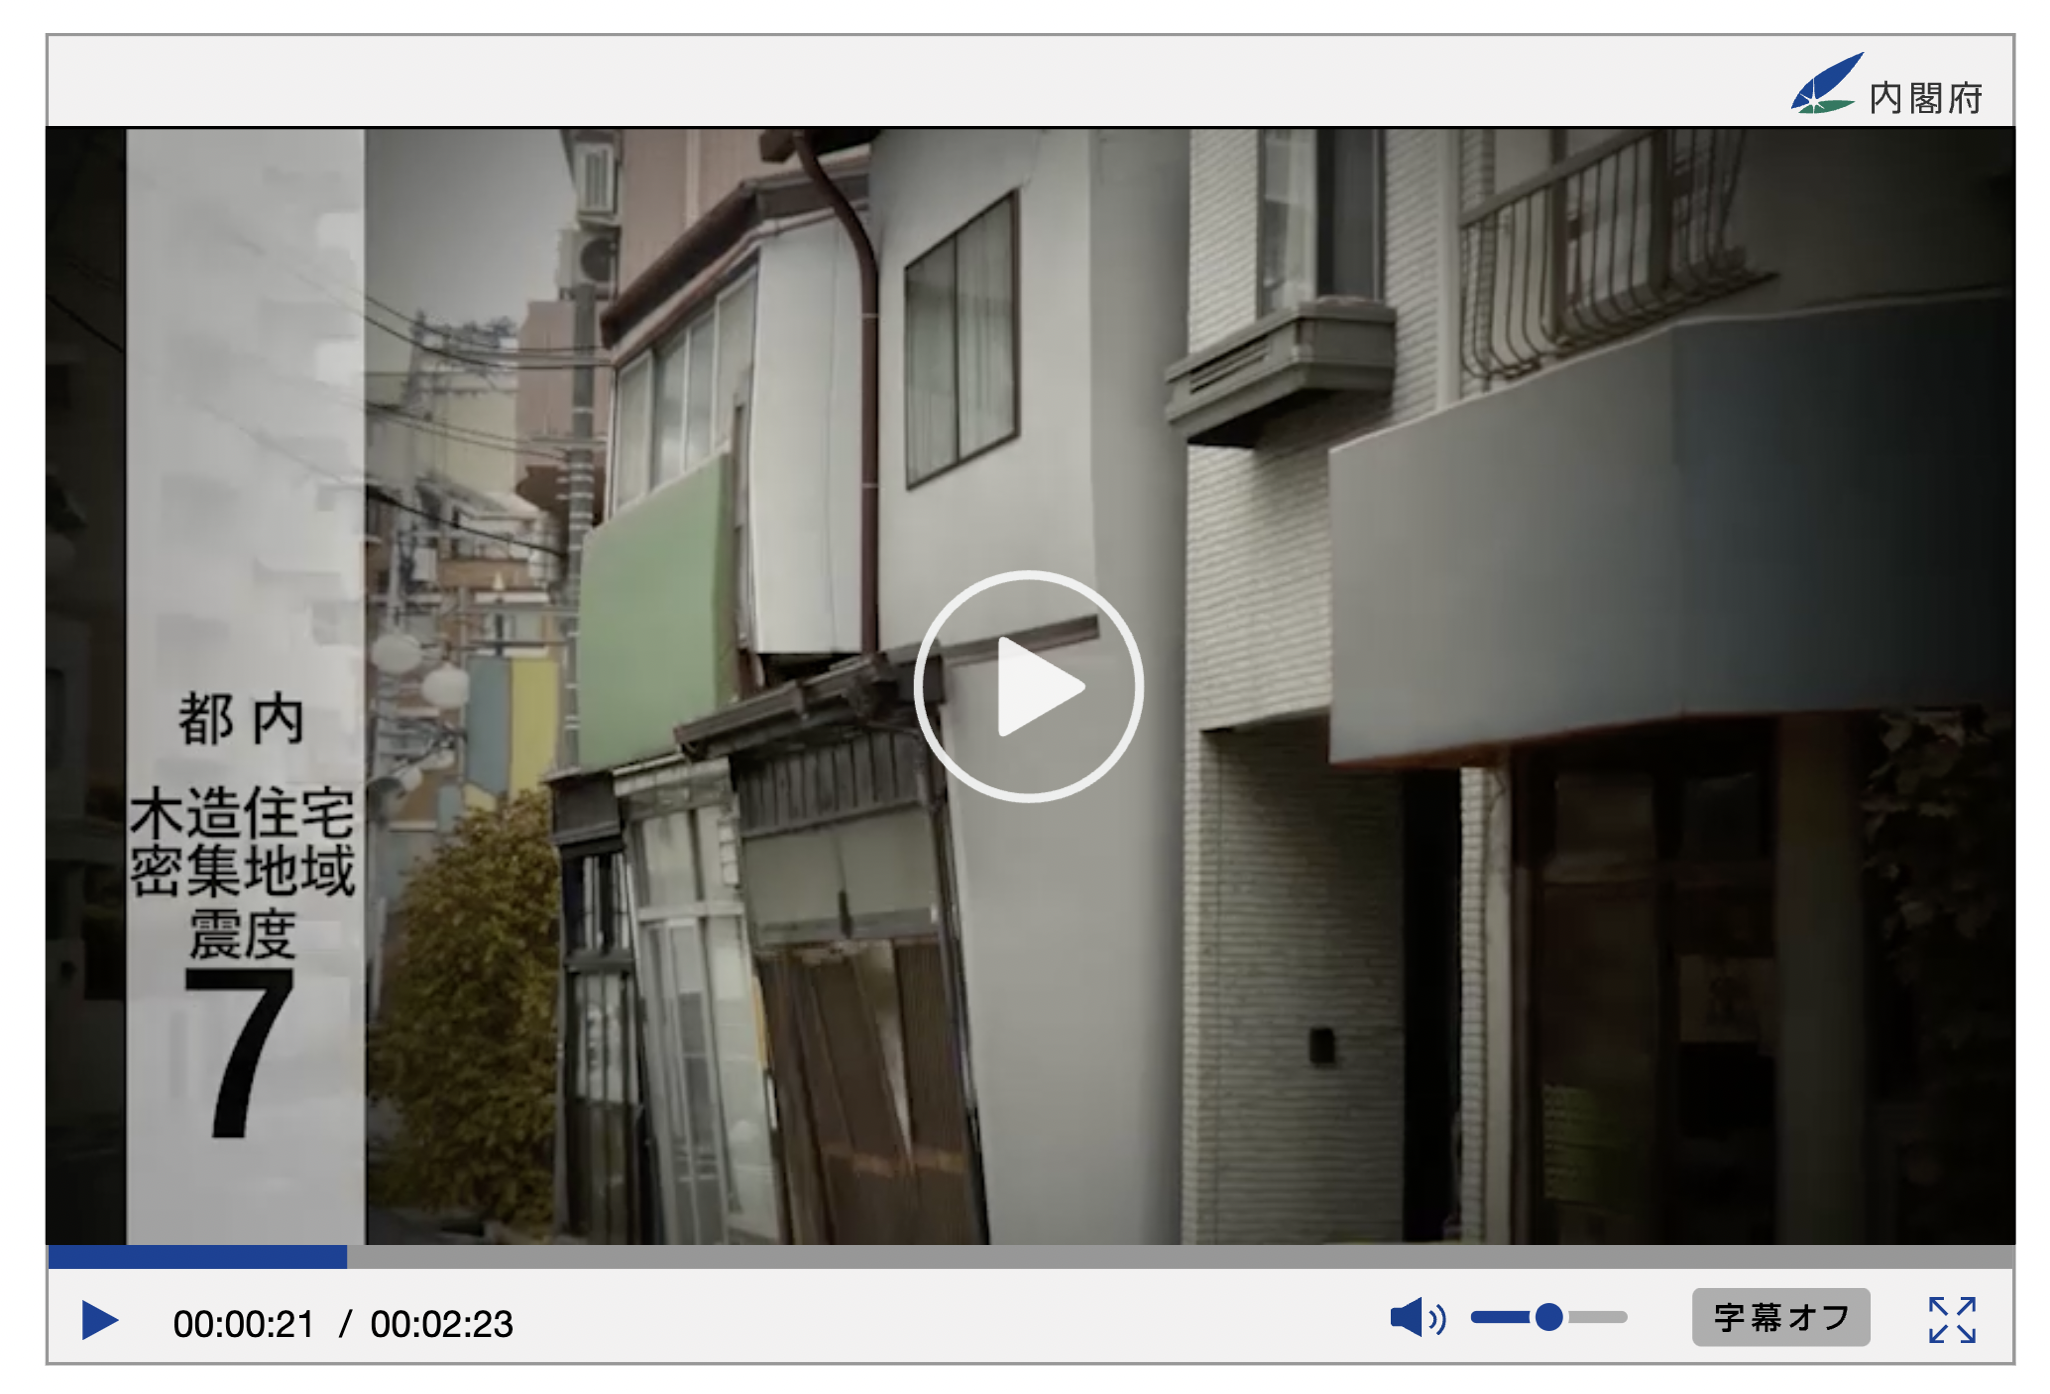
\includegraphics[width=\linewidth]{Figure/Figure5d.jpg}
    \caption{Tokyo-Wooden houses (Dense area); Seismic intensity 7}
    \label{fig5d}
  \end{subfigure}\hfill
  \begin{subfigure}{0.32\textwidth}
    \centering
    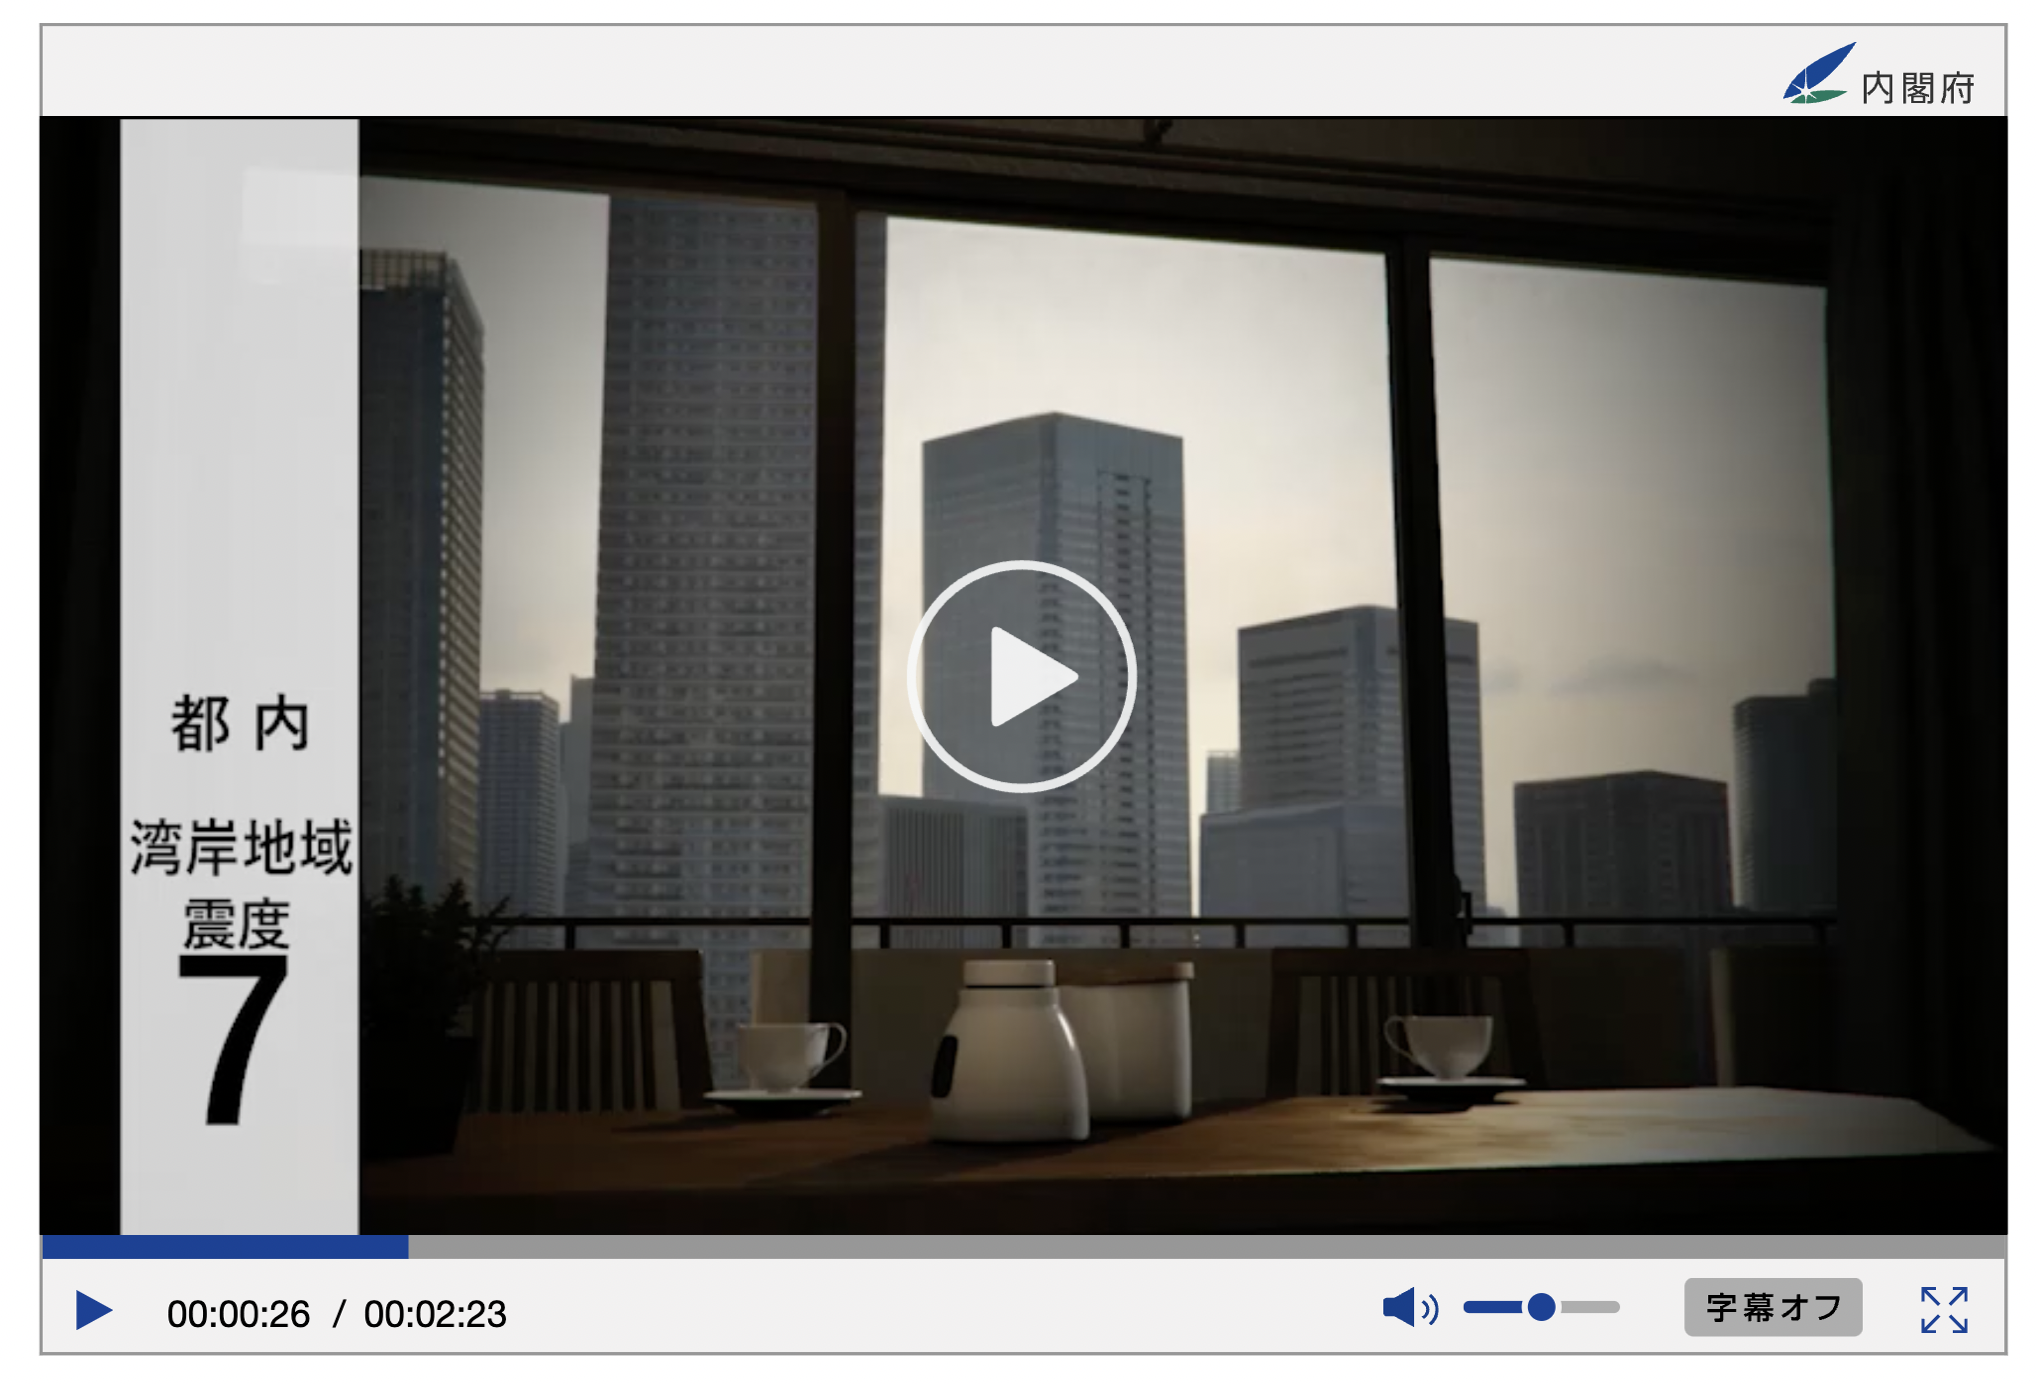
\includegraphics[width=\linewidth]{Figure/Figure5e.jpg}
    \caption{Tokyo-Bay Area; Seismic intensity 7}
    \label{fig5e}
  \end{subfigure}\hfill
  \begin{subfigure}{0.32\textwidth}
    \centering
    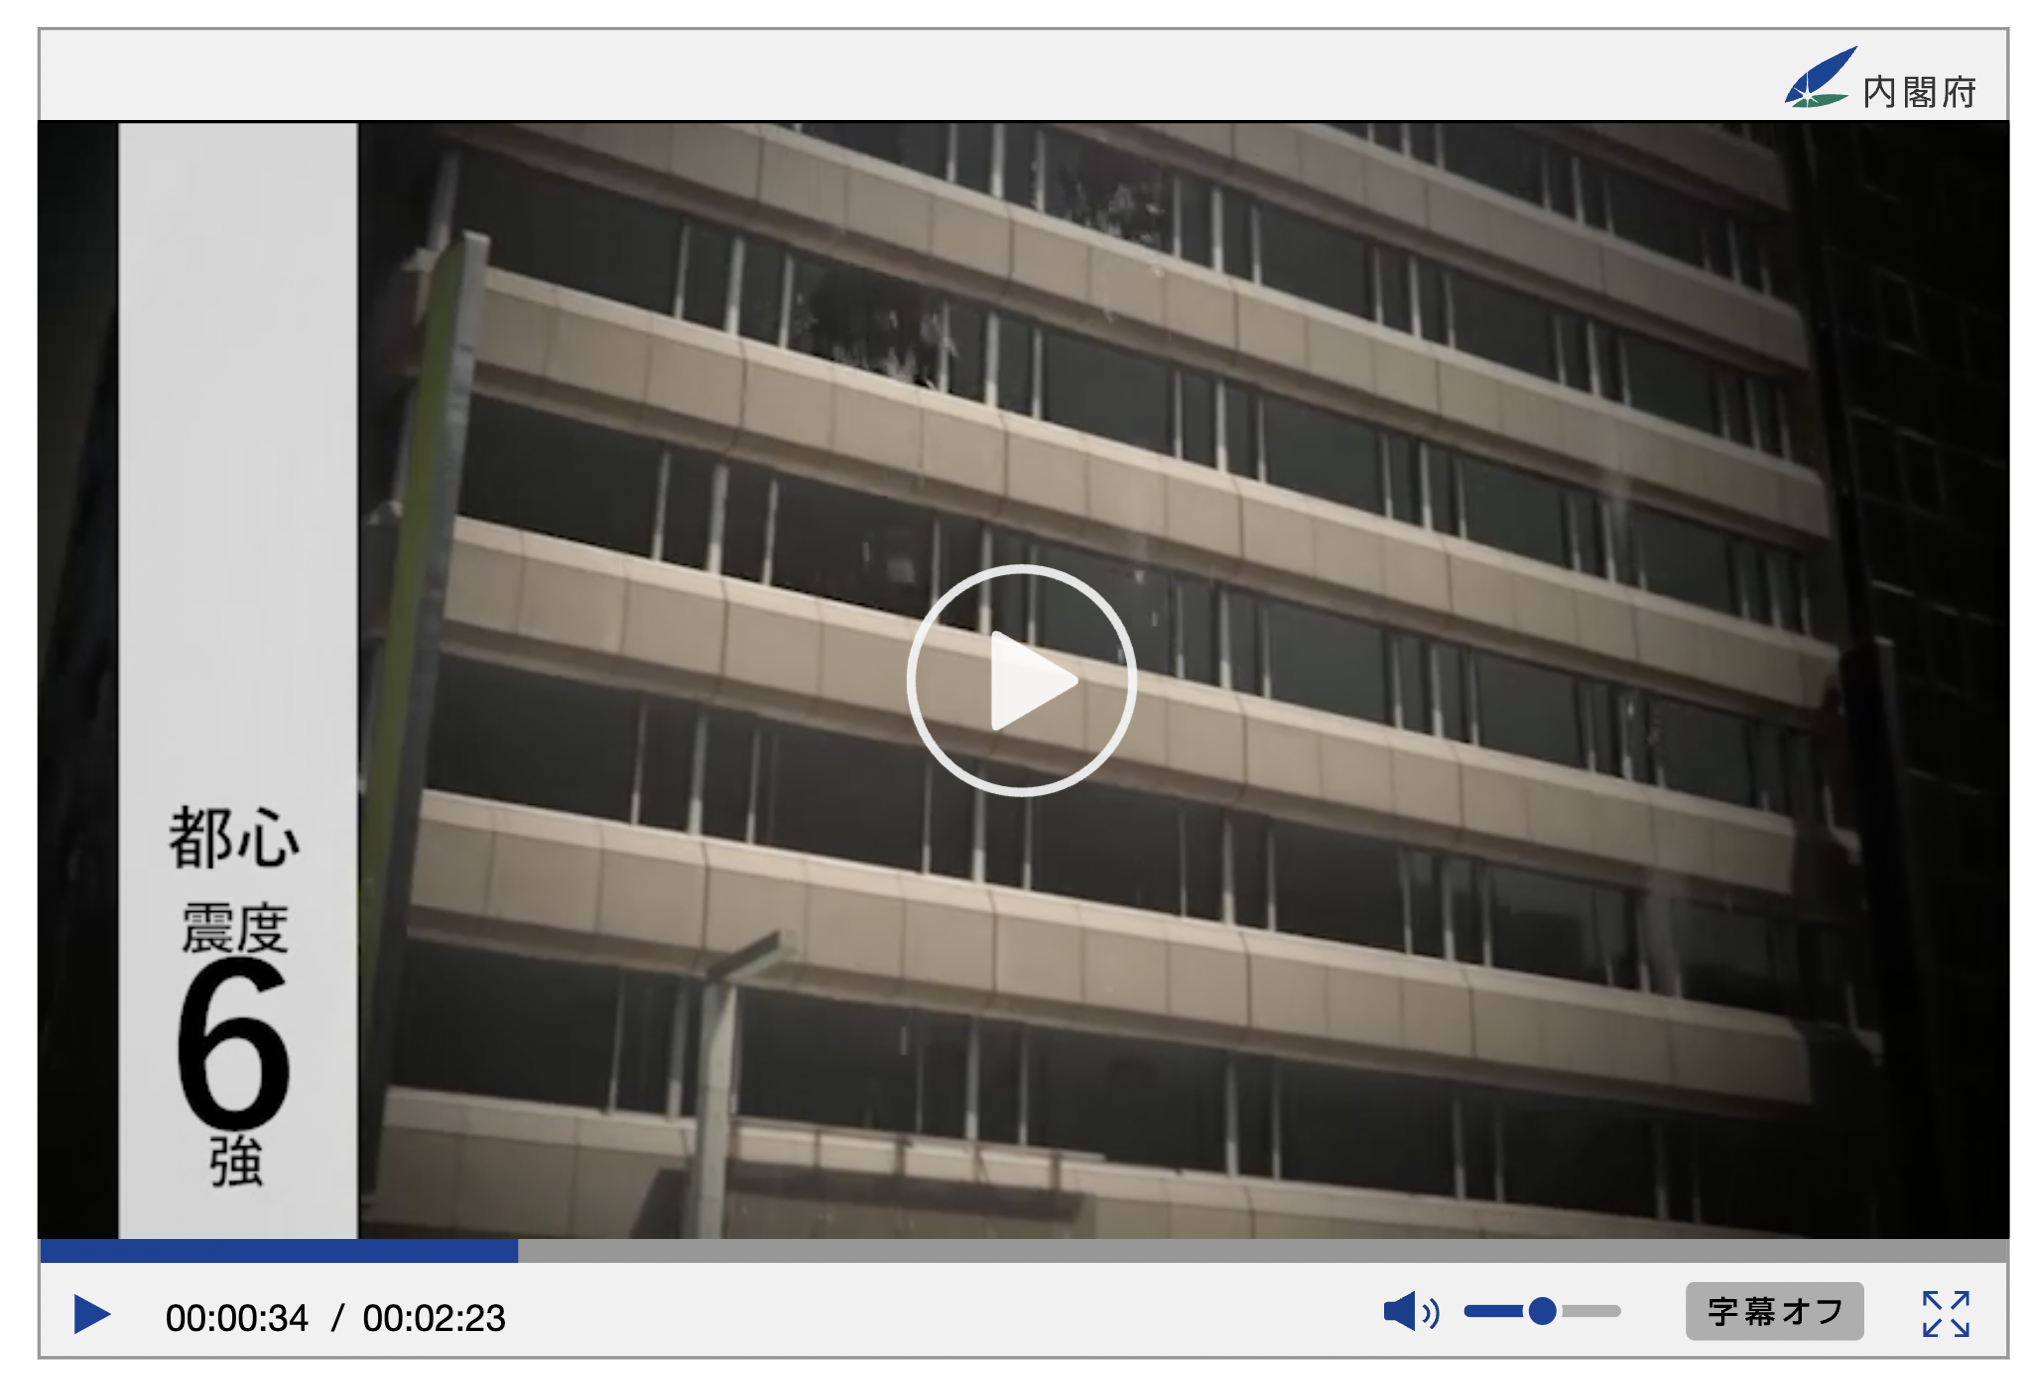
\includegraphics[width=\linewidth]{Figure/Figure5f.jpg}
    \caption{Tokyo; Seismic intensity 6-}
    \label{fig5f}
  \end{subfigure}
  \begin{subfigure}{0.32\textwidth}
    \centering
    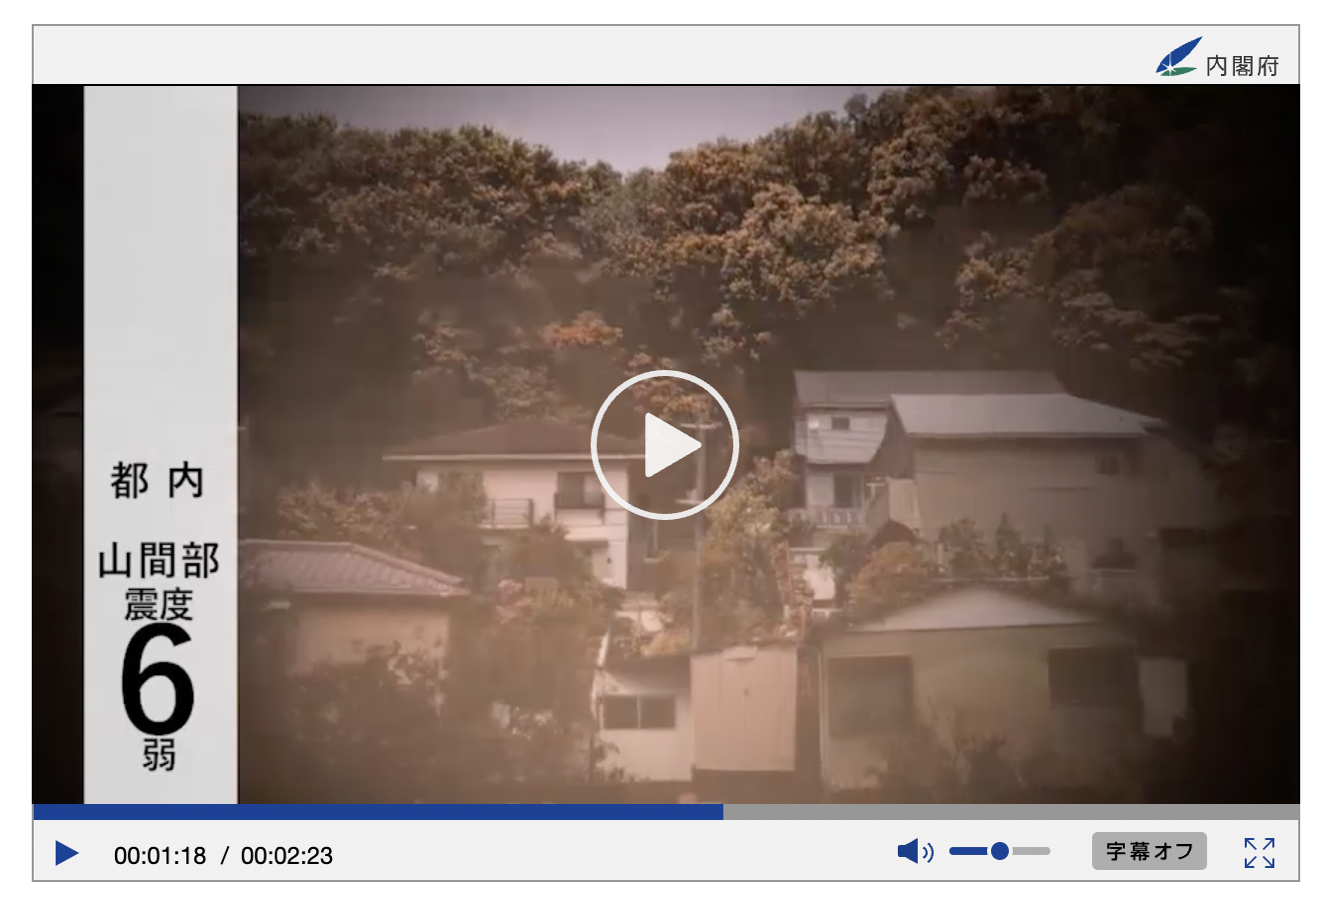
\includegraphics[width=\linewidth]{Figure/Figure5g.jpg}
    \caption{Tokyo-Mountainous region; Seismic intensity 6+}
    \label{fig5g}
  \end{subfigure}
  \centering
  \caption[Simulation video of  "Tokyo Metropolitan Earthquake".]{Simulation video of "Tokyo Metropolitan Earthquake".\protect\footnotemark }
  \label{fig5}
\end{figure*}
 \footnotetext{http://wwwc.cao.go.jp/lib\_012/syuto\_02.html}
%\fi



%% Some LaTeX commands I define for my own nomenclature.
% If you have to, it's better to change nomenclature once here than in a 
% million places throughout your thesis!



%======================================================================
\chapter{Methodology }
%======================================================================

\section{Methodology for achieving Objective - 1 }

\textbf{Objective 1: To understand foreign visitors' attitudes toward Safety Tips.}

 For research objective 1, the nationality data in item 1 and item 6 were used, containing three tasks. While considering that the main users of Safety Tips are foreign visitors, only the sample of foreign respondents was selected for this part of the analysis, and the sample of Japanese respondents was excluded in this part. So the total number of samples was 1500.

The first task is to summarize the questionnaire's results from Q15 to Q17. The findings will show the popularity, experience, and attitude of Safety Tips in each country, as well as the differences among respondents from 5 countries.

The second question was based on the answers to Q15 and Q16, and all respondents were divided into five groups. Q15 was "do you know Safety tips or not?", and Q16 was "Did you use safety tips before or not?". The answers to Q15 had three options: Know exactly, Heard safety tips before, and Do not know. If the respondent answered "Know exactly" or "Heard Safety tips before", the respondent will continue to answer Q16, if the respondent answers "Do not know", the respondent will directly skip to Q17. The answers to Q16 are "used Safety tips before." and "never used it before". Therefore, the respondents were divided into the following five groups: "Know exactly and used Safety tips before", "Know exactly but never used Safety tips before.", "Heard Safety tips before and used it before", "Heard Safety tips before but never used it before", and "Do not know and never used before". The sample sizes for each group are shown in Figure~\ref{fig6}, which are "Know exactly and used Safety tips before": 357; "Know exactly but never used Safety tips before": 90; "Heard Safety tips before and used it before": 134; "Heard Safety tips before but never used it before": 465 people; "Do not know and never used before": 454 people. The results will show whether the two factors of respondents' past awareness and whether they used it before had an impact on their attitudes toward Safety Tips.

\begin{figure*}[h]
  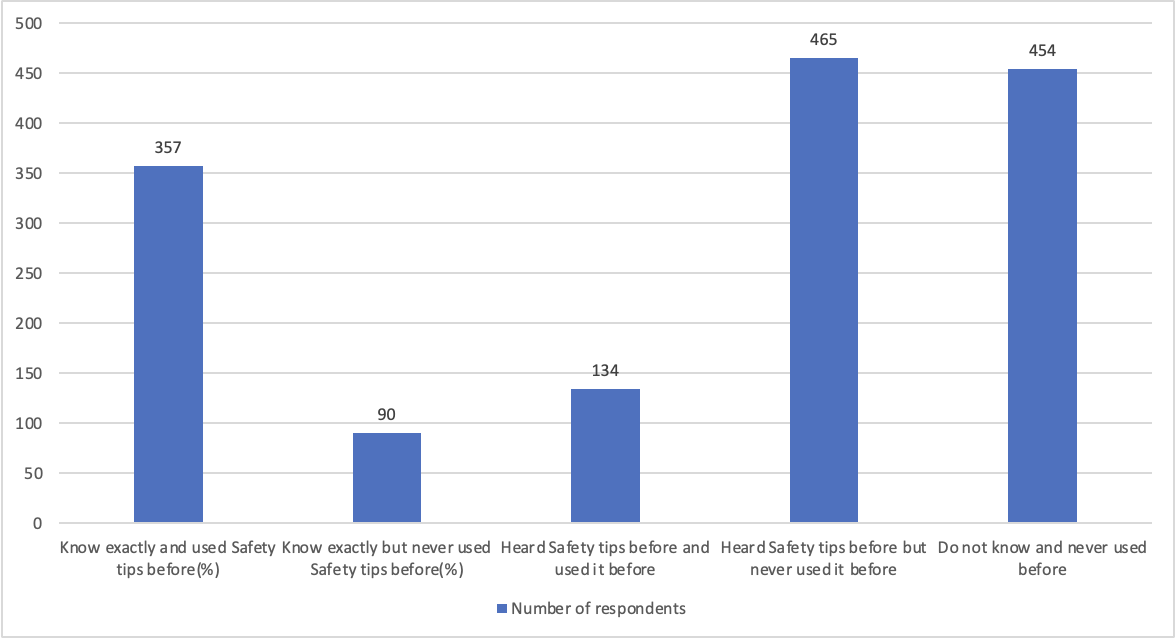
\includegraphics[width=\linewidth]{Figure/Figure6.jpg}
  \centering
  \caption{Number of respondents in each group. }
  \label{fig6}
\end{figure*}

The third task is an independent sample t-test analysis. The responses of Q15 and Q16 were used to test whether the responses of the respondents to the four questions of Q17 were significantly different because of the difference between Q15 and Q16. The independent sample t-test analysis of Q15 versus Q17\_1, Q17\_2, Q17\_3, and Q17\_4 examined whether there were significant differences in the attitudes toward Safety Tips between respondents who were previously aware of Safety Tips and those who were previously unaware of Safety Tips. Independent sample t-tests for Q16 and Q17\_1, Q17\_2, Q17\_3, and Q17\_4 were conducted to examine whether there was a significant difference in attitudes toward Safety Tips between respondents who had previously used Safety Tips and those who had not used Safety Tips.


\section{Methodology for achieving Objective - 2 }
\textbf{Objective 2: To explore how respondents' attitudes toward Safety Tips are influenced by their characteristics. }

For research purpose 2, the data of Item 1, Item 2-4, and Item 6 were used. This part will continue to look into the impact of respondents' personality characteristics on their attitude toward Safety Tips. As a consequence, the study still uses a sample size of 1500 foreign visitors.

Structural Equation Modeling will be used to analyze this part. Structural Equation Modeling is a statistical method based on Regression Models for Latent Variables. Structural Equation Modeling can consider and deal with multiple dependent variables at the same time and allow for measurement error in both independent and dependent variables. Also, Structural Equation Modeling can estimate both factor structure and factor relationships, which could be more useful for this research. Therefore, this study will use Structural Equation Modeling to explore whether factors such as respondents' personal characteristics, disaster consciousness, disaster experience, and disaster training experience will have an impact on respondents' attitudes toward Safety Tips or not. Like \#Table 5 shows, there are four Latent variables, which are Disaster Prevention Consciousness, Disaster Knowledge, and Attitude toward Safety Tips. The latent variable "Disaster Prevention" has 5 manifest variables, which are Disastrous Imagination (Q1), Sense of crisis (Q2), Other-directed type (Q3), Anxiety (Q4), Apathy about disasters (Q5). The latent variable "Disaster knowledge" has 2 manifest variables, which are Knowledge about earthquakes (Q9) and Knowledge of how to respond to a disaster (Q10). The latent variable "Training experiences" has 2 manifest variables, which are the Total score of earthquake/tsunami/typhoon/fire training experiences. (Q6) and Number of times participating in earthquake/tsunami/typhoon/fire disaster training (Q7). The latent variable "Attitude on Safety Tips" has 2 manifest variables, which are Trust level (Q17\_1), Priority of use (Q17\_2), Usefulness (Q17\_3), and Possibility of future use (Q17\_4). There are another 6 manifest variables, which are Age (FQ3), Gender (FQ2), Number of visits to Japan within 1 year (FQ5), Number of visits to any country in the world within 1 year (FQ4), Japanese level (FQ7), and Number of experienced earthquakes (Q8).

\subsection{Hypothesis for SEM}

In order to construct Structural Equation Modeling for this research, it is necessary to make hypothesizes based on previous research.  

\begin{itemize}
\item Individual characteristics (risk belief, connectedness, knowledge, and past experience with hurricanes), travel-related variables, and the socio-demographic characteristics of tourists influence their decision regarding whether or not to evacuate in the event of a hurricane.~\cite{Cahyanto2014AnEE}
\item The tourists' evacuations were also influenced by tourists' hurricane knowledge and past experience.~\cite{Cahyanto2016StatedPO}
\end{itemize}

Base on these two studies, we can construct a relationship that knowledge, travel-related variables, and socio-demographic characteristics could relate to Evacuation Behaviors, shown in Figure~\ref{fig7}. 

\begin{figure*}[h]
  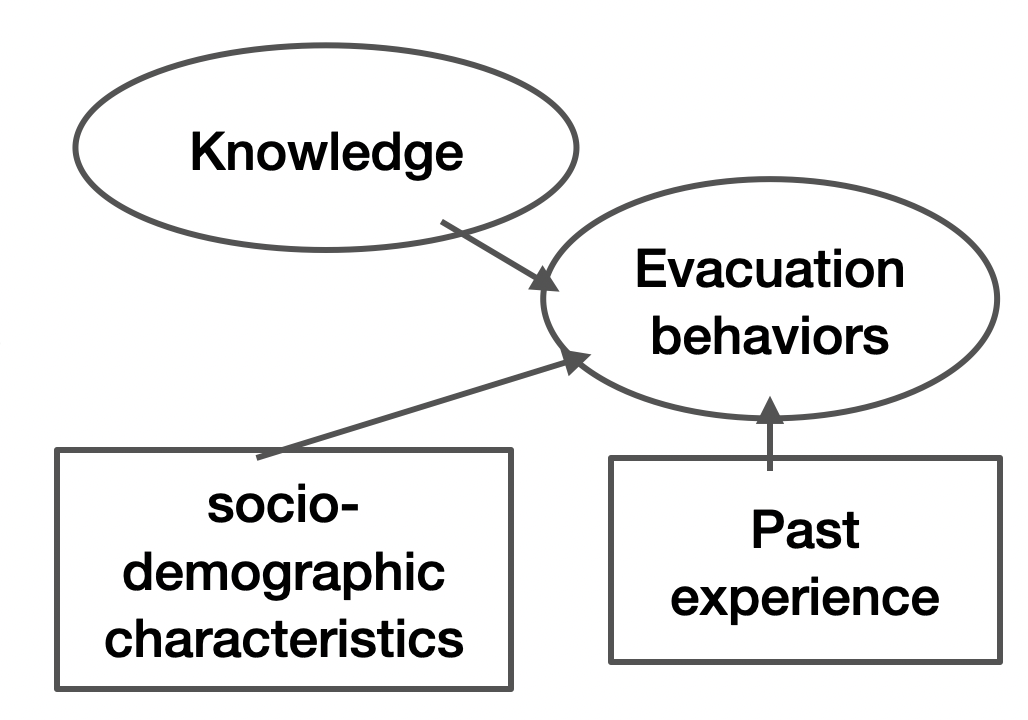
\includegraphics[width=0.5\linewidth]{Figure/Figure7.png}
  \centering
  \caption{Hypothesis base on previous research - 1 }
  \label{fig7}
\end{figure*}

\begin{itemize}
\item Evacuation is significantly related to Socio-demographic factors, such as age, gender, etc, Socioeconomic factors, like educational attainment or household characteristics, etc, Personal characteristics, like hazard experience, knowledge, abilities/impairments, etc. Also, evacuees tend to make use of their familiarity with the surroundings based on their knowledge.~\cite{Wang2021IncorporatingHF}
\end{itemize}

Base on this study, we can construct a relationship that age, gender, hazard experience,  educational attainment, knowledge, abilities could relate to Evacuation Behaviors, shown in Figure~\ref{fig8}. 

\begin{figure*}[h]
  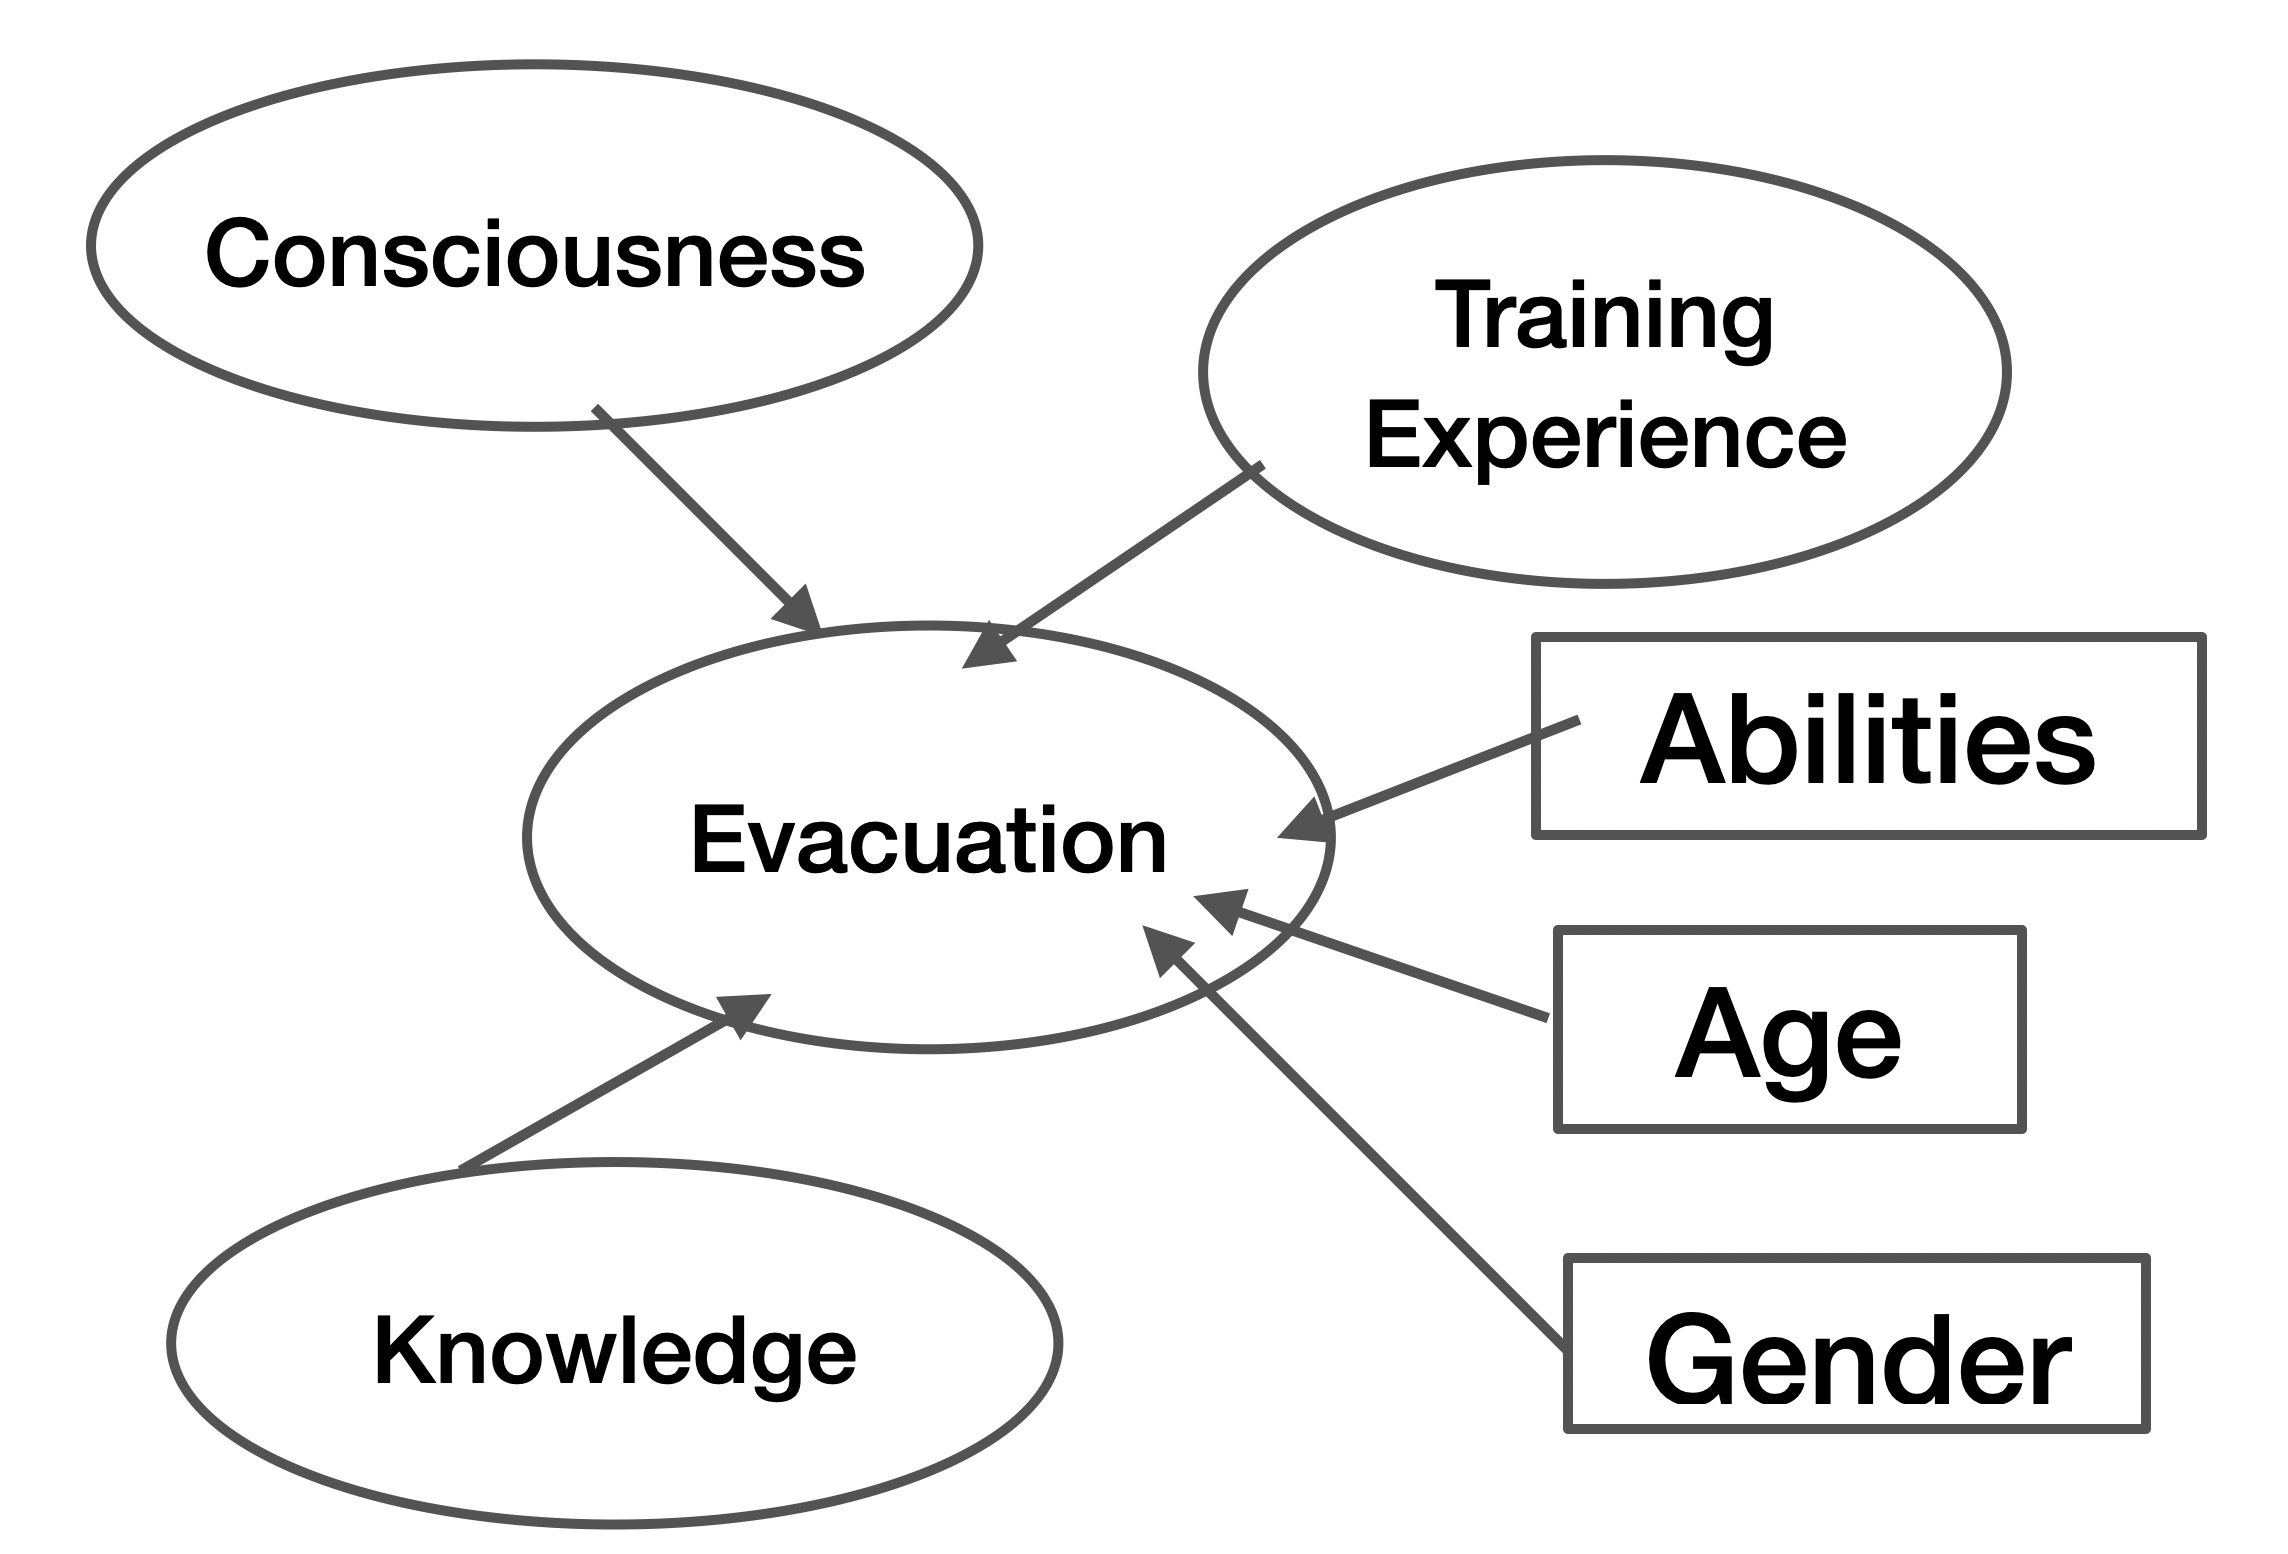
\includegraphics[width=0.5\linewidth]{Figure/Figure8.png}
  \centering
  \caption{Hypothesis base on previous research - 2 }
  \label{fig8}
\end{figure*}

By combining these hypothesizes, we finally construct an SEM model, shown in Figure~\ref{fig9}. 

\begin{figure*}[h]
  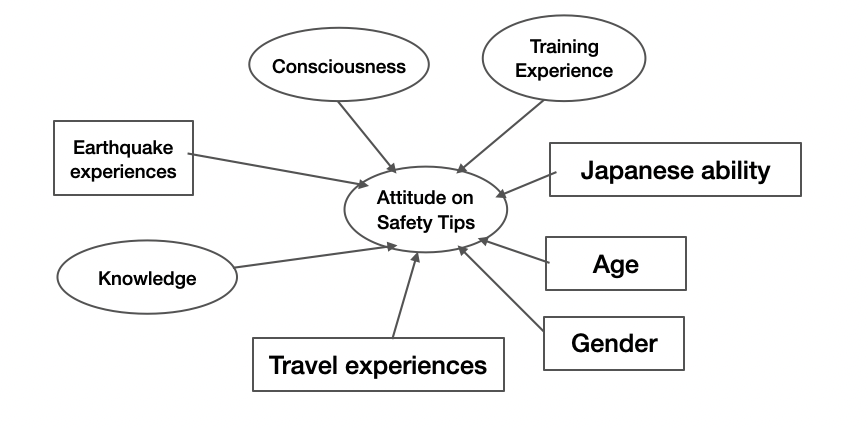
\includegraphics[width=\linewidth]{Figure/Figure9.png}
  \centering
  \caption{Final Hypothesis used for SEM }
  \label{fig9}
\end{figure*}

\subsection{Data Processing}
\begin{itemize}
\item Item 1 (FQ2-FQ5,FQ7)
\end{itemize}

FQ2: $(Male) = 1$; $(Female) = 2$;

FQ3: $(Age Under 15) = 1$; $(Age 16-19) = 2$; $(Age 20-29) = 3$; $(Age 30-39) = 4$; $(Age 40-49) = 5$; $(Age 50-59) = 6$; $(Age 60-69) = 7$; $(Age Over 70) = 8$;

FQ4\&FQ5: number means the time of visit country/Japan;

FQ7: $(Cannot understand) = 1$; $(Basic) = 2$; $(Intermediate) = 3$; $(Up Level) = 4$; 

\begin{itemize}
\item Item 2 (Q1-Q5)
\end{itemize}

Since each of Q1-Q5 has four sub-problems. Here will use the mean values of the four sub-problems as the final data. For example, Q1 = $mean$ (Q1\_1, Q1\_2, Q1\_3, Q1\_4), Q2-Q5 are processed in the same way.

\begin{itemize}
\item Item 3 (Q6-Q8)
\end{itemize}

Q6 is about past disaster training participation experience. There are four types of disasters: Q6\_1 earthquake, Q6\_2 tsunami, Q6\_3 typhoon, and Q6\_4 fire. Each of them has 12 different types of training experience, shown as Q6\_1/2/3/4\_1 to Q6\_1/2/3/4\_12. Respondents answered with 'Yes' or 'No' in these questions. If none of them were experienced before, 'Yes' was selected in Q6\_1/2/3/4\_13 to indicate that the respondent did not have any of the 12 experiences mentioned above. 

Therefore, 

Q6\_1 = $sum$ (Q6\_1\_1 + Q6\_1\_2 +... + Q6\_1\_12);

Q6\_2 = $sum$ (Q6\_2\_1 + Q6\_2\_2 +... + Q6\_2\_12);

Q6\_3 = $sum$ (Q6\_3\_1 + Q6\_3\_2 +... + Q6\_3\_12);

Q6\_4 = $sum$ (Q6\_4\_1 + Q6\_4\_2 +... + Q6\_4\_12).

Q7 is times of past disaster training experiences. There are also four types of disasters: Q7\_1 earthquake, Q7\_2 tsunami, Q7\_3 typhoon, and Q7\_4 fire.
 
(one time) = 1; (2-3 times) = 2; (4-6 times) = 3; (Over 7 times) =4;

\begin{itemize}
\item Item 4 (Q9-Q10)
\end{itemize}

Q9 has six sub-problems, Q10 has nine sub-problems. Here will use the mean values of the sub-problems as the final data. 

Therefore, 

Q9 = $mean$ (Q9\_1, Q9\_2, ... , Q9\_6);

Q10 = $mean$ (Q10\_1, Q10\_2, ... , Q10\_9).

\begin{itemize}
\item Item 6 (Q15-Q17)
\end{itemize}

Q15: (Don't know) = 1; (Only heard name before) = 2; (Know exactly) = 3;

Q16: (Never used before) = 0; (Used before) = 1;
 
Q17\_1, Q17\_2, Q17\_3, Q17\_4: use orginal data.


\section{Methodology for achieving Objective - 3}

\textbf{Objective 3: To explore patterns of information seeking and evacuation behaviors.}

For research objective 3, this study wanted to explore respondents' information-seeking behaviors and evacuation behaviors through their selections of behaviors. In order to understand which of the behaviors are preferred and which are selected more frequently, we chose to measure both the selected rate and the selected score. The calculation of the selected rate and the selected score will both do three times, for 300 Japanese samples, 1500 foreign visitors samples, and 1800 of all respondents' samples.

\subsection{Selected Rate}
Because the selected rate wants to explore which behaviors are used more, this part does not take the order factor into account. No matter the behavior is selected in which order, it will count as 1 point. The selected rate is equal to the Sum selected point divided by the sample number, shown in Figure~\ref{fig10}.

\begin{figure*}[h]
  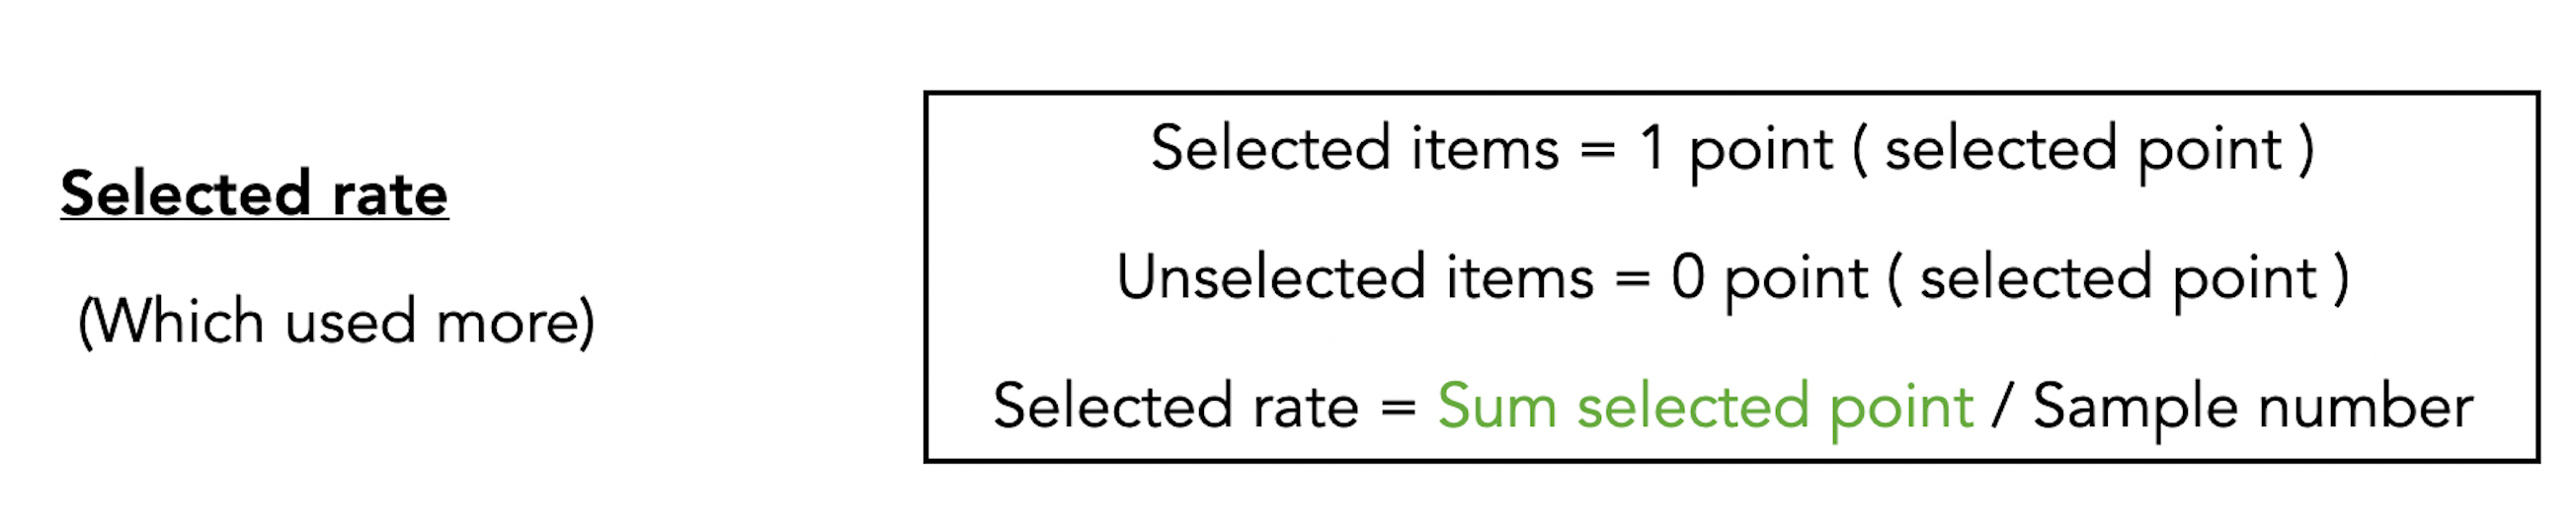
\includegraphics[width=\linewidth]{Figure/Figure10.png}
  \centering
  \caption{Selected rate }
  \label{fig10}
\end{figure*}

\subsection{Selected Score}

Since the Selected score wants to explore which behaviors are used first, this part needs to take the order factor into account. The higher the preference is, the higher the score will be. So the first selected action is scored as 5, the second is scored as 4, the third is scored as 3, the fourth is scored as 2, and the last selected action is scored as 1. The Selected score is equal to the total score divided by the Sum selected point, shown in Figure~\ref{fig11}.

\begin{figure*}[h]
  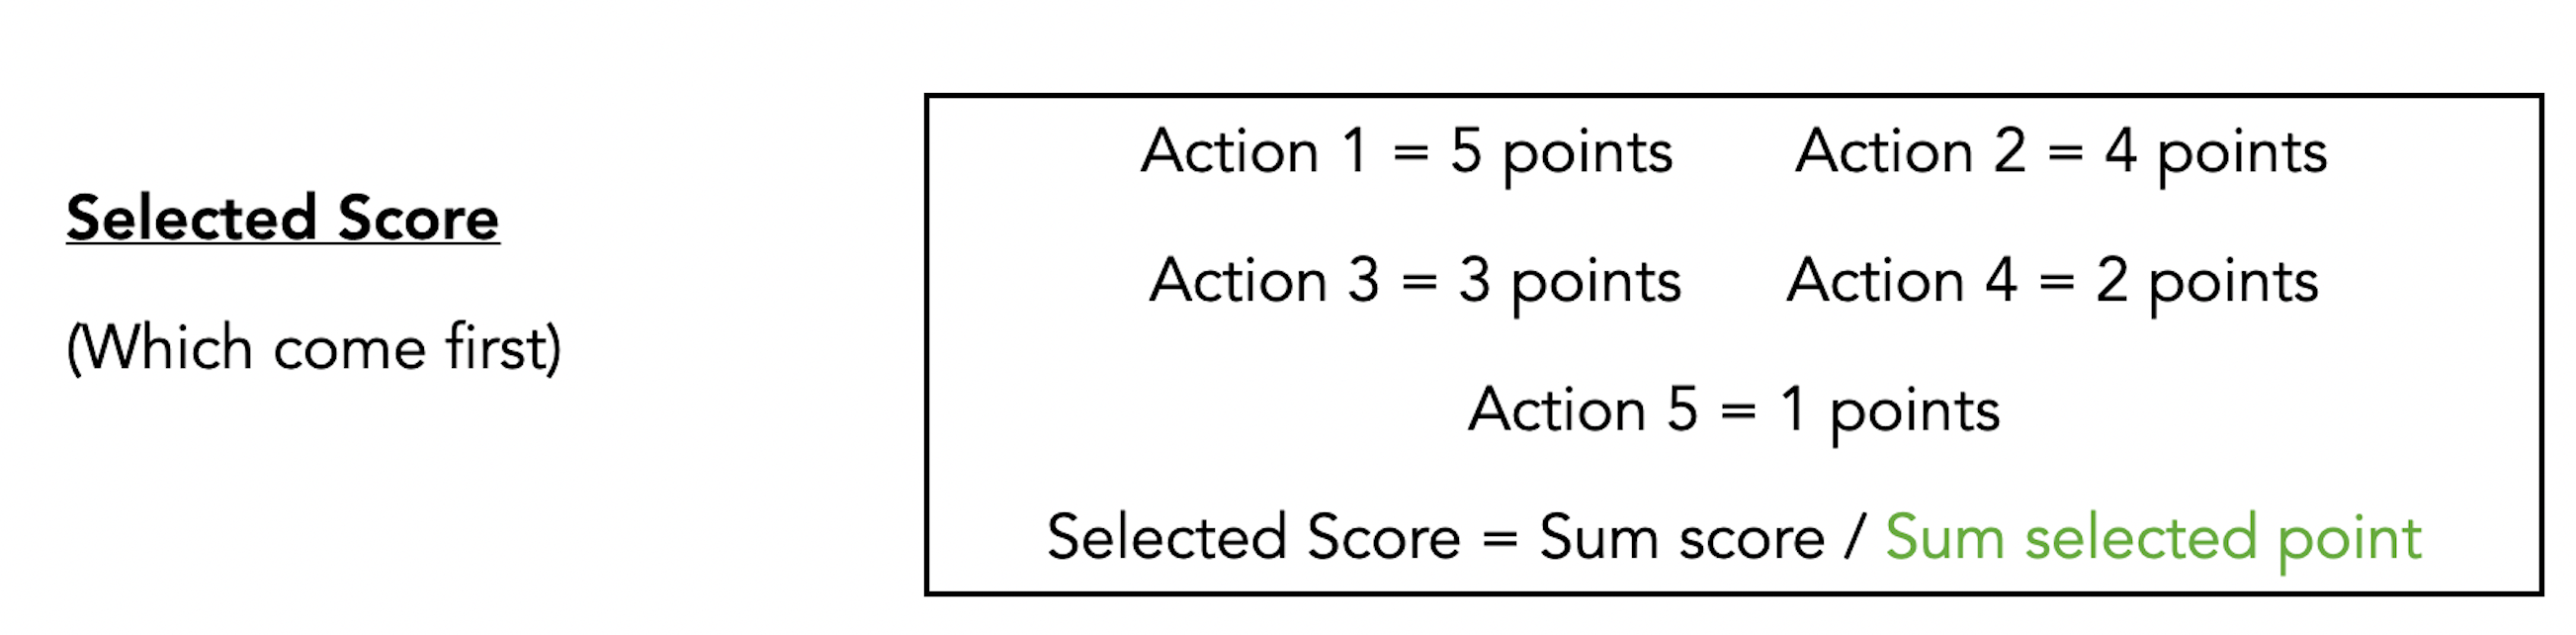
\includegraphics[width=\linewidth]{Figure/Figure11.png}
  \centering
  \caption{Selected score}
  \label{fig11}
\end{figure*}

\subsection{Behavior Pattern}

In the analysis of the selected score and selected rate of study objective 3, we will find that all the results will be relatively scattered. This is because, in this study, the number of available selections is relatively large, which makes the results more scattered. However, from the results, we can see that there could be similarities in the behavior patterns of people. Here the word "pattern" means behavior patterns, not specific behavior. For example, the behavior of  "collecting information" is the same, the difference is how to collect information, from official websites, from disaster prevention software, from disaster prevention websites, from SNS, etc. So how to divide detailed behaviors into patterns? From the available selection, we can find that the behavior is mainly divided into two kinds, which are information-seeking behavior and evacuation behavior. First, regarding information-seeking behavior, we can find that there are two main patterns, one is "No-face-to-face information seeking" and the other is "Face-to-face information seeking". And for the evacuation behavior, we can also find two main patterns, one is " Self-evacuation behaviors " and the other is " Following evacuation guidance behavior ". Then, we divided all the selections into the patterns they belong to, which can be found in Figure~\ref{fig12}.

\begin{figure*}[h]
  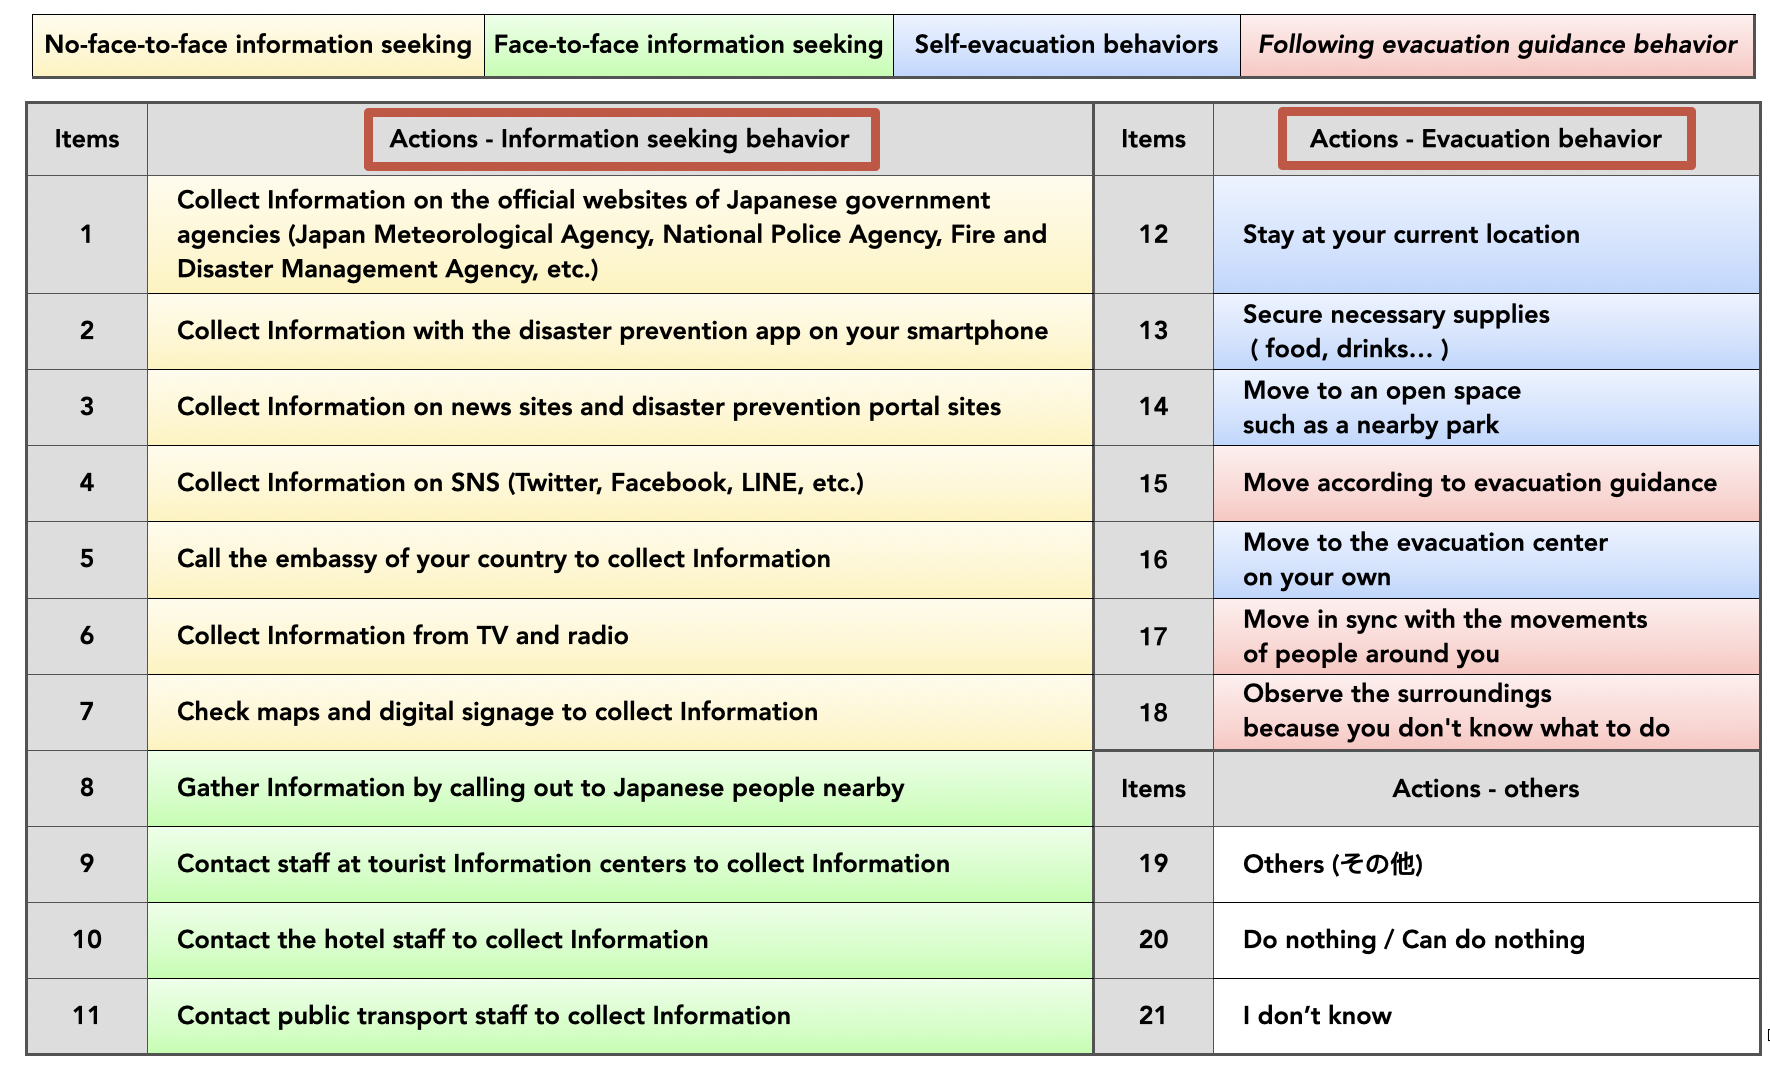
\includegraphics[width=\linewidth]{Figure/Figure12.png}
  \centering
  \caption{behavior patterns}
  \label{fig12}
\end{figure*}

After attributing all the actions to the 4 patterns, we went through the flow of the respondents' actions with the help of the Sankey Program. The Sankey Program is a flow chart that shows the flow from each set of values to another set of values. The thickness of the lines expresses the number of values present in the group. In the Sankey Program, the number indicates the No. of action, so 1-5 means the first action to the fifth action. Capital letters indicate behavior patterns." No-face-to-face information seeking" is A; "Face-to-face information seeking" is B; "Self-evacuation behaviors" is C; "Following evacuation guidance behavior" is D. Thus, the behavior from the first to the fifth cohort can be clearly represented in the results of the Sankey Program. As an example, A1 indicates that the 1st response action during the disaster is behavior pattern A, which is "No-face-to-face information seeking".





























% Some LaTeX commands I define for my own nomenclature.
% If you have to, it's better to change nomenclature once here than in a 
% million places throughout your thesis!
%======================================================================
\chapter{Results and Discussion}
\label{c5}
%======================================================================

\section{Results for Objective 1 }
\subsection{First Task}
For Q15, do the respondents know about SafetyTips before, the result is shown in Figure~\ref{fig13}. we can find that around 50\% of the respondents from the UK and Korea do not know Safety Tips before, around 80\% of the respondents from China and Thailand know or at least heard Safety Tips before, while around 90\% of the respondents from Indonesia know or at least heard Safety Tips before. 

\begin{figure*}[h]
  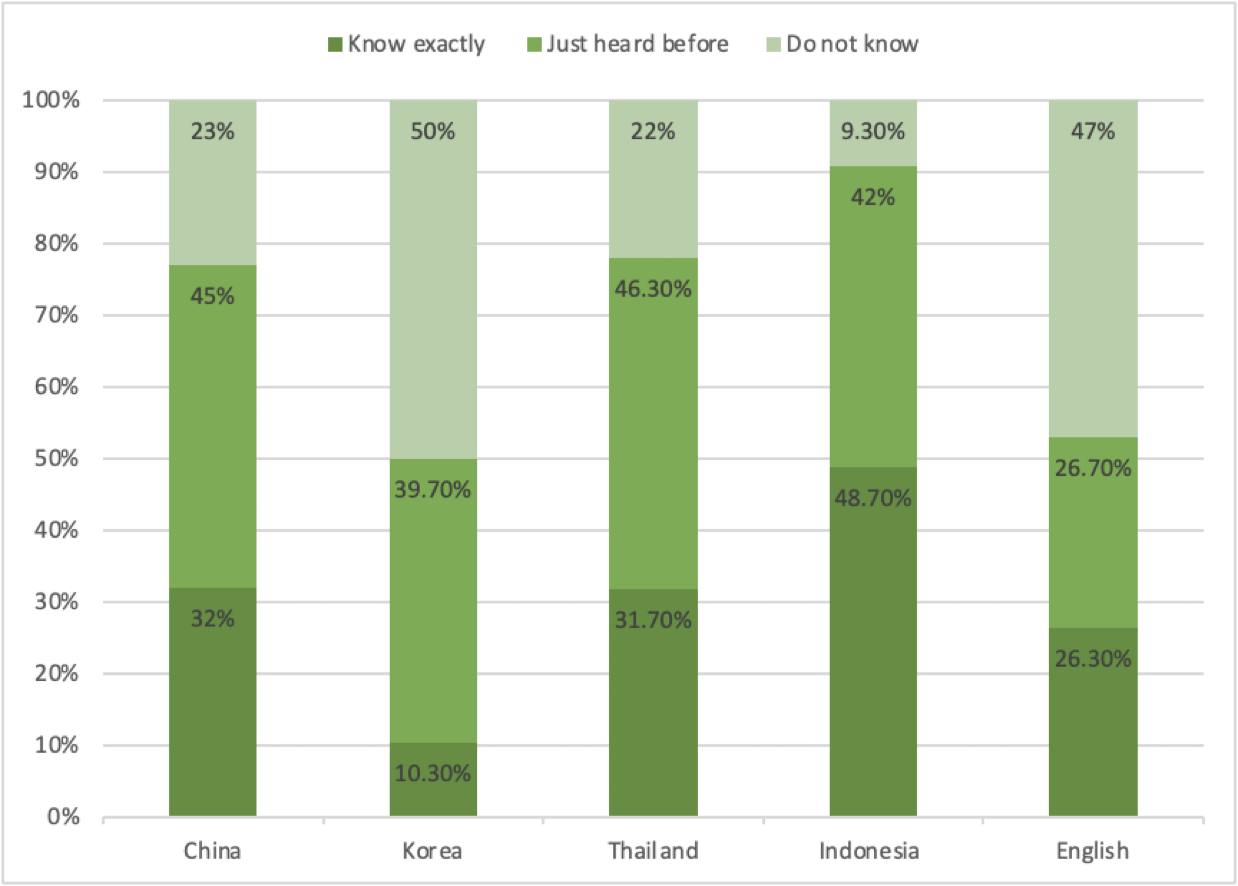
\includegraphics[width=0.8\linewidth]{Figure/Figure13.jpg}
  \centering
  \caption[Survey result of Q15]{Survey result of Q15(Do you know Safety Tips or not ?)}
  \label{fig13}
\end{figure*}

For Q16, did the respondents use SafetyTips before, the result shows in Figure~\ref{fig14}. we can find that more than 50\% of the respondents from China(66.2\%), Korea(72\%), and Thailand(55.1\%) did not use Safety Tips before, while more than 50\% of respondents from Indonesia(65.8\%) and the UK(54.7\%) have used Safety Tips before. Among all countries, respondents from Indonesia have the highest usage rate of Safety Tips at 65.8\%. Koreans had the lowest, at 28\%. 

\begin{figure*}[h]
  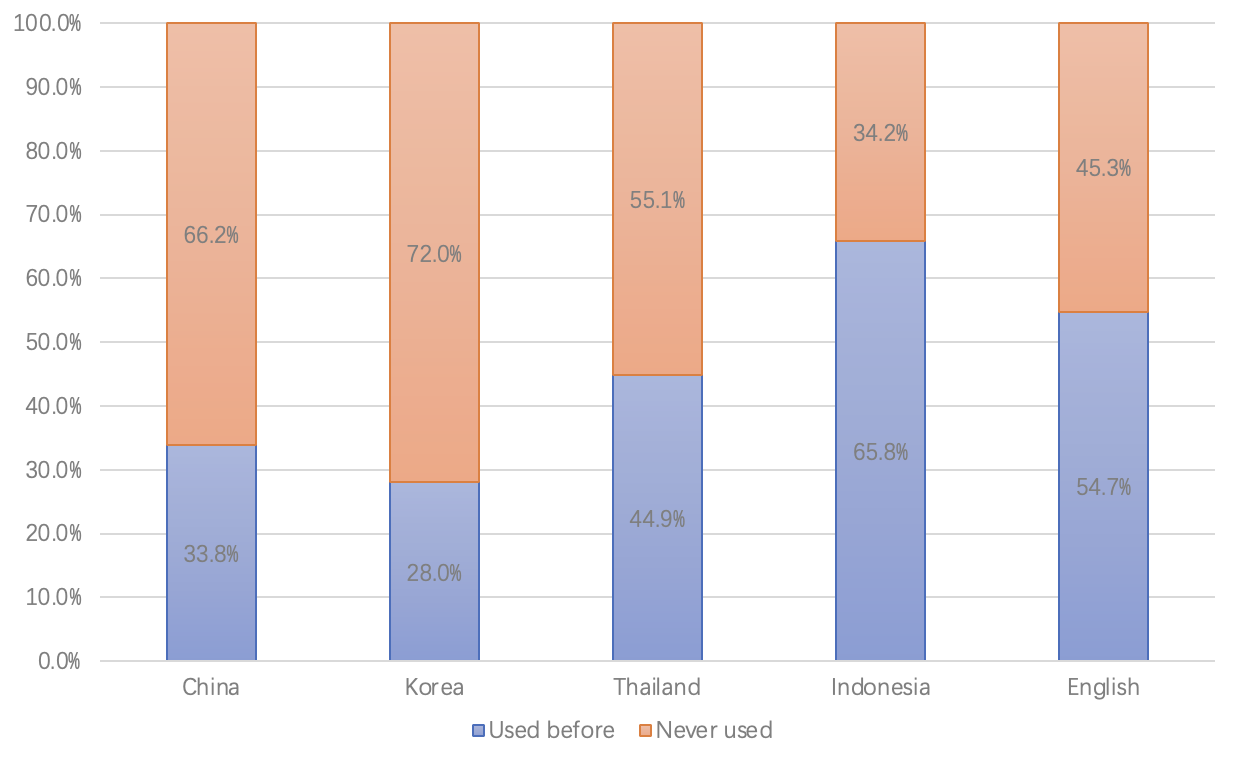
\includegraphics[width=0.8\linewidth]{Figure/Figure14.jpg}
  \centering
  \caption[Survey result of Q16]{Survey result of Q16(Do you use Safety Tips before or not ?)}
  \label{fig14}
\end{figure*}

For Q17\_1, Will the respondents trust Safety Tips more than information from their country, the result shows in Figure~\ref{fig15}. we can find that over 90\% of respondents from Thailand(91.1\%) and Indonesia(91.7\%) said they trusted information from Safety Tips more than from their own countries, and more than 80\% of respondents from China(80.3\%) feel that the information on Safety Tips could be trusted more than their own countries, while respondents from the UK(78\%) and Korea(77.3\%) have a relatively low level of trust in Safety Tips compared to the other three countries, but still around 70\%. 

\begin{figure*}[h]
  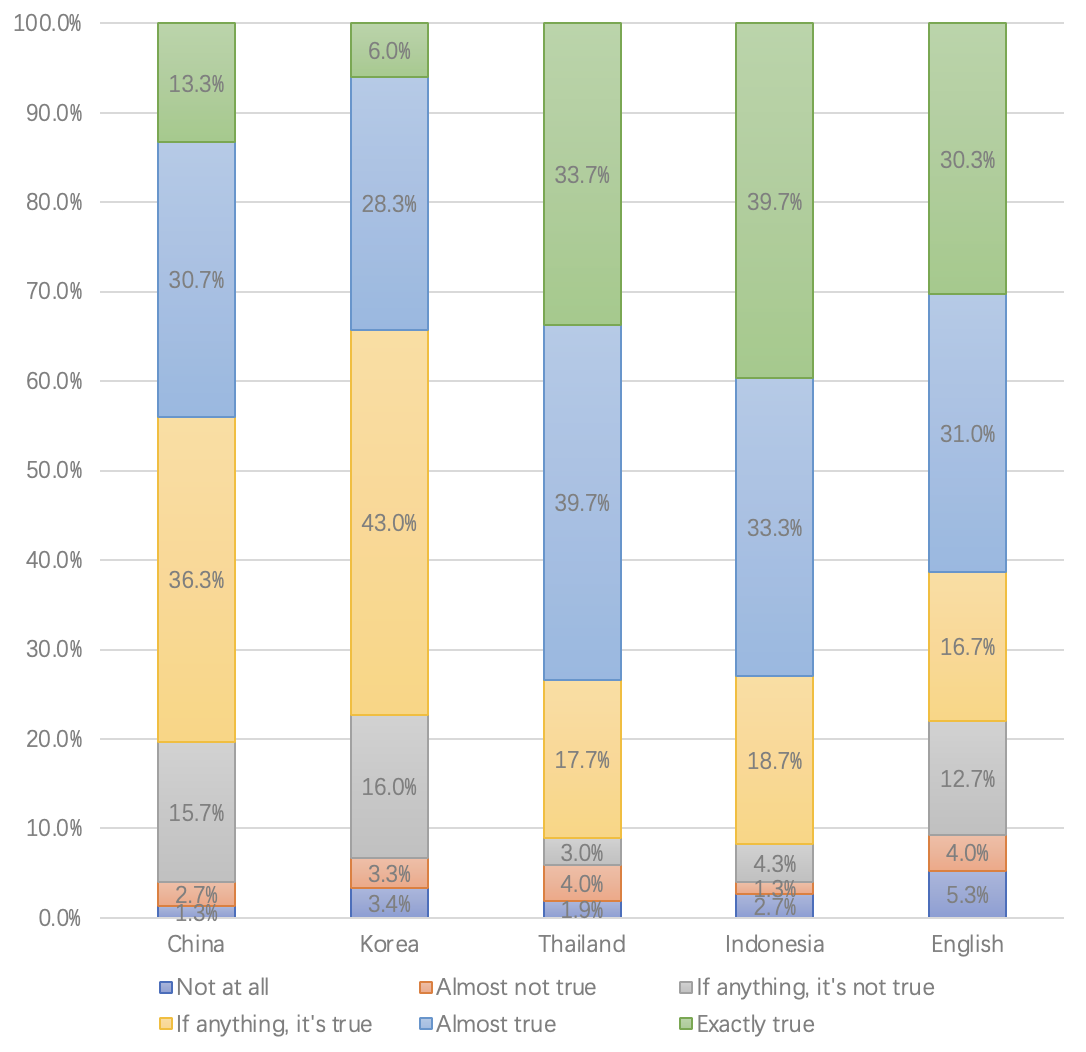
\includegraphics[width=0.8\linewidth]{Figure/Figure15.jpg}
  \centering
  \caption[Survey result of Q17\_1]{Survey result of Q17\_1(Will you trust Safety Tips more than information from your own country ?)}
  \label{fig15}
\end{figure*}

For Q17\_2, Will the respondents use Safety Tips before searching information from their country, the result shows in Figure~\ref{fig16}. we can find that over 90\% of respondents from Thailand(90.7\%) and Indonesia(94.1\%) said they use Safety Tips to search information before their own country's, and more than 80\% of respondents from China(88\%), the UK(82.3\%) and Korea(82.3\%) will use Safety Tips to find information before their own country. 

\begin{figure*}[h]
  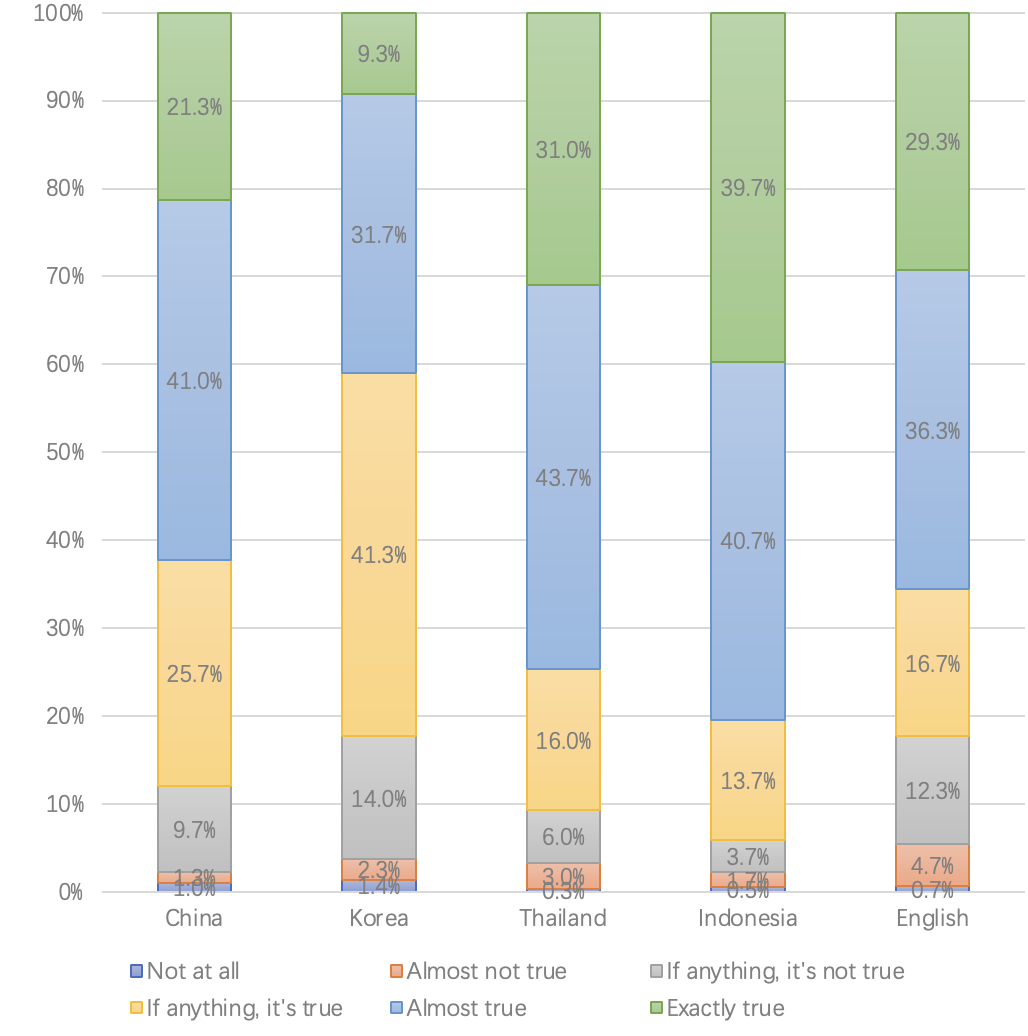
\includegraphics[width=0.8\linewidth]{Figure/Figure16.jpg}
  \centering
  \caption[Survey result of Q17\_2]{Survey result of Q17\_2(Will you use Safety Tips before searching information from your own country ?)}
  \label{fig16}
\end{figure*}

For Q17\_3, do the respondents think Safety Tips could be useful during the evacuation, the result is shown in Figure~\ref{fig17}. we can find that over 90\% of respondents from Thailand(95.4\%), China(95.7\%), and Indonesia(96.6\%) think Safety Tips could be useful during the evacuation, and more than 80\% of respondents from the UK(87\%) and Korea(84.9\%) think Safety Tips could be useful during evacuation. 

\begin{figure*}[h]
  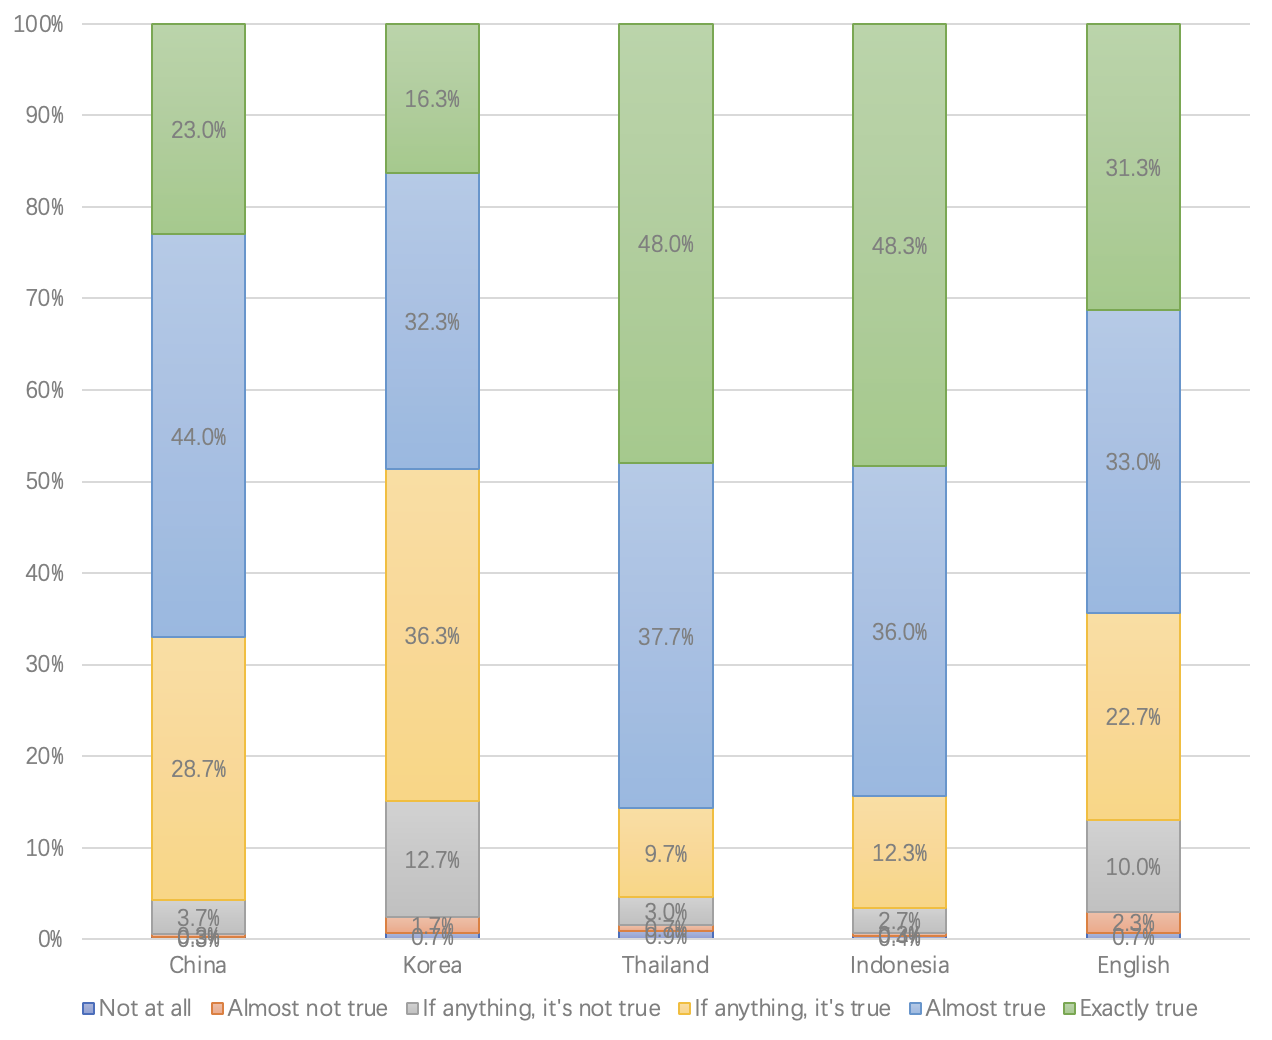
\includegraphics[width=0.8\linewidth]{Figure/Figure17.jpg}
  \centering
  \caption[Survey result of Q17\_3]{Survey result of Q17\_3(Do you think Safety Tips could be useful during evacuation ?)}
  \label{fig17}
\end{figure*}

For Q17\_4, will the respondents use Safety Tips in the future, the result shows in Figure~\ref{fig18}. we can find that over 90\% of respondents from Thailand(93.3\%), China(95.3\%), and Indonesia(95.3\%) think they will use Safety Tips in the future, and more than 80\% of respondents from the UK(87\%) and Korea(84.9\%) think they will use Safety Tips in the future.

\begin{figure*}[h]
  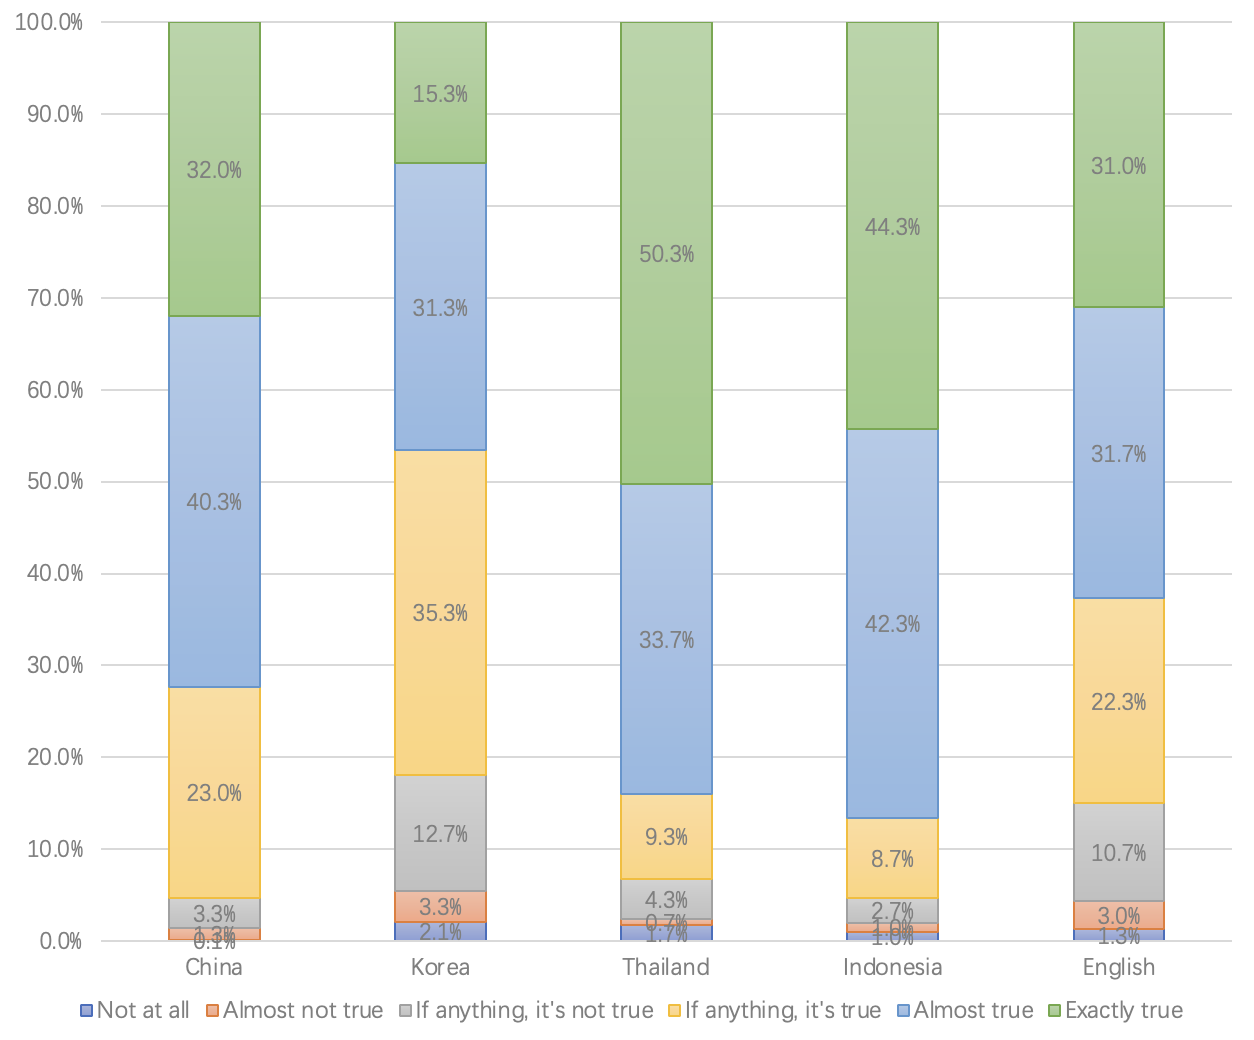
\includegraphics[width=0.8\linewidth]{Figure/Figure18.jpg}
  \centering
  \caption[Survey result of Q17\_4]{Survey result of Q17\_4(Will you use Safety Tips in the future ?)}
  \label{fig18}
\end{figure*}

From the above results, we can conclude that from the usage experience, Safety Tips could be more popular and well-known in Indonesia(90\%), China(77\%), and Thailand(79\%) rather than in the UK(53\%) and Korea(50\%). Also, among those respondents that know Safety Tips or heard them before, their usage rate is lower than 70\%. China(33.8\%), Korea(28\%), Thailand(44.9\%), Indonesia(65.8\%) and the UK(54.7\%). Then from the attitude toward Safety Tips, we can conclude that over 77\% of the respondents say that they trust Safety Tips more than information from their own countries, over 82\% of the respondents say that they will use Safety Tips to search information before from their own countries, and over 84\% of the respondents say that they believe Safety Tips could be useful during evacuation and will use Safety Tips in the future.

\subsection{Second Task}
In the second task, we aim to find whether the two factors of respondents' past awareness and whether they used it before had an impact on their attitudes toward Safety Tips. After dividing all respondents into 5 groups, we can find the differences between groups. 

For Q17\_1, Will the respondents trust Safety Tips more than information from their country, the result shows in Figure~\ref{fig19}. we can find that respondents who know exactly and used Safety Tips before have shown the highest trust toward Safety Tips, as more than 75\% of the respondents said they trust the information on Safety Tips rather than from their own countries. Respondents who know exactly but never used Safety Tips before and respondents who heard Safety Tips before but never used Safety Tips before are more likely to trust the information on Safety Tips. Respondents who heard and used Safety Tips before and respondents who do not know and never used this application before have shown a relatively negative attitude toward Safety Tips. 

\begin{figure*}[h]
  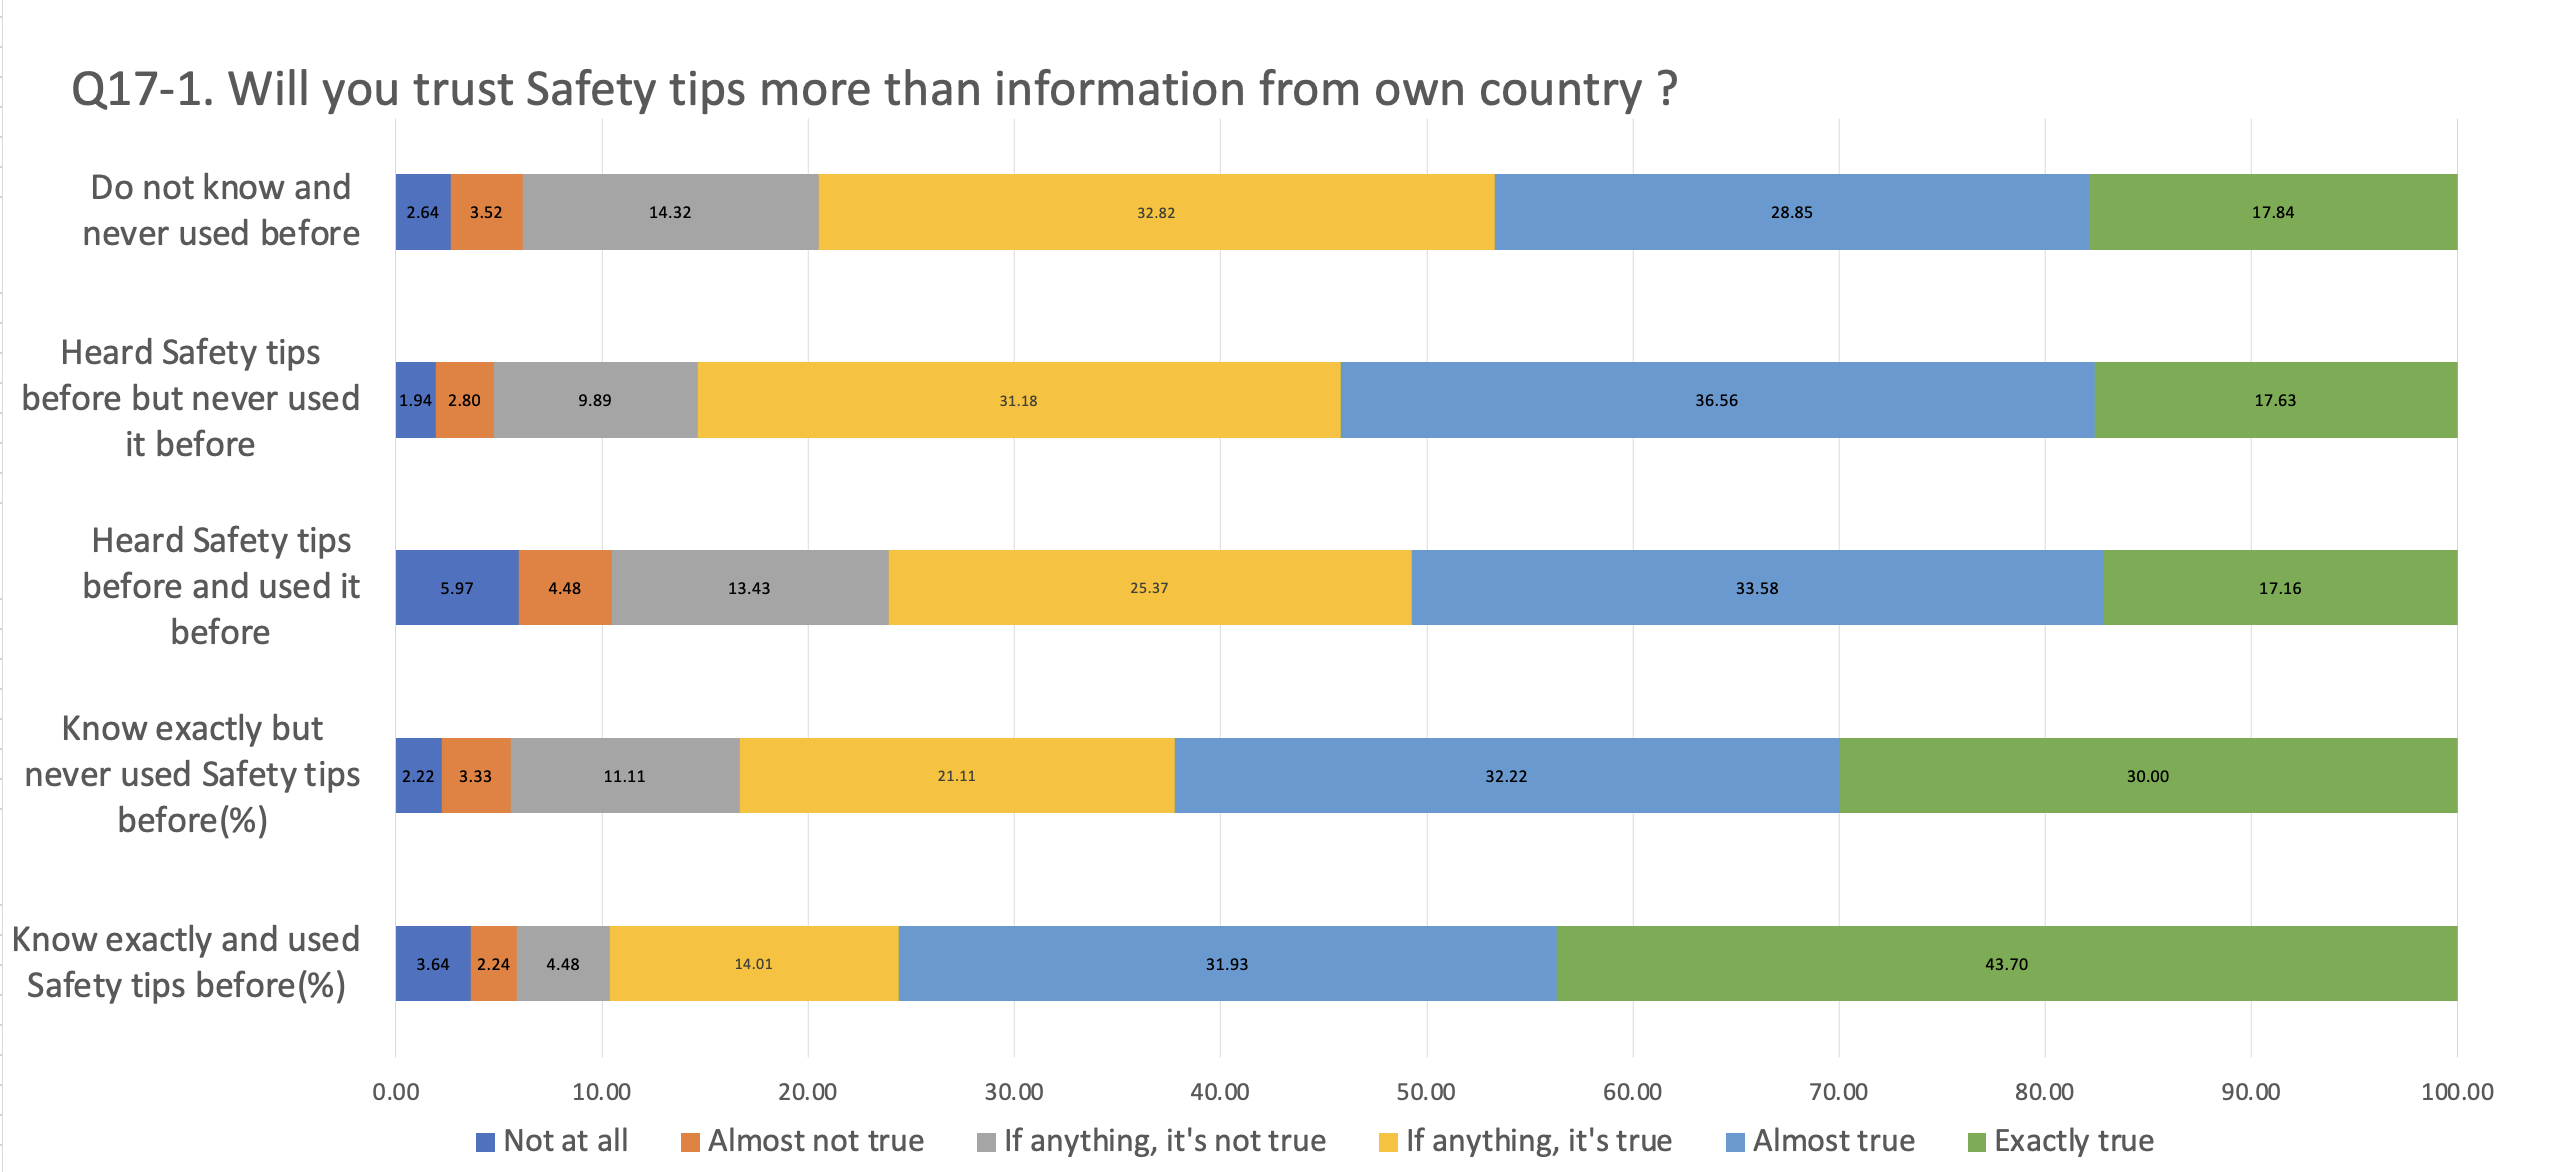
\includegraphics[width=0.8\linewidth]{Figure/Figure19.jpg}
  \centering
  \caption[5 groups of respondents' survey result of Q17\_1]{5 groups of respondents' survey result of Q17\_1(Will you trust Safety Tips more than information from your own country ?)}
  \label{fig19}
\end{figure*}

For Q17\_2, Will the respondents use Safety Tips before searching information from their country, the result shows in Figure~\ref{fig20}. we can find that the respondents who know exactly and used Safety Tips before have shown the highest usage possibility on Safety Tips, as more than 80\% of the respondents said Safety Tips have a higher priority of usage rather than from their own countries. Respondents that know exactly but never used Safety Tips before and respondents who heard Safety Tips before but never used Safety Tips before have shown similar attitudes on the priority of using Safety Tips. Respondents who do not know and never used before and respondents who heard Safety Tips before and used Safety Tips before have shown a little bit lower usage priority. 

\begin{figure*}[h]
  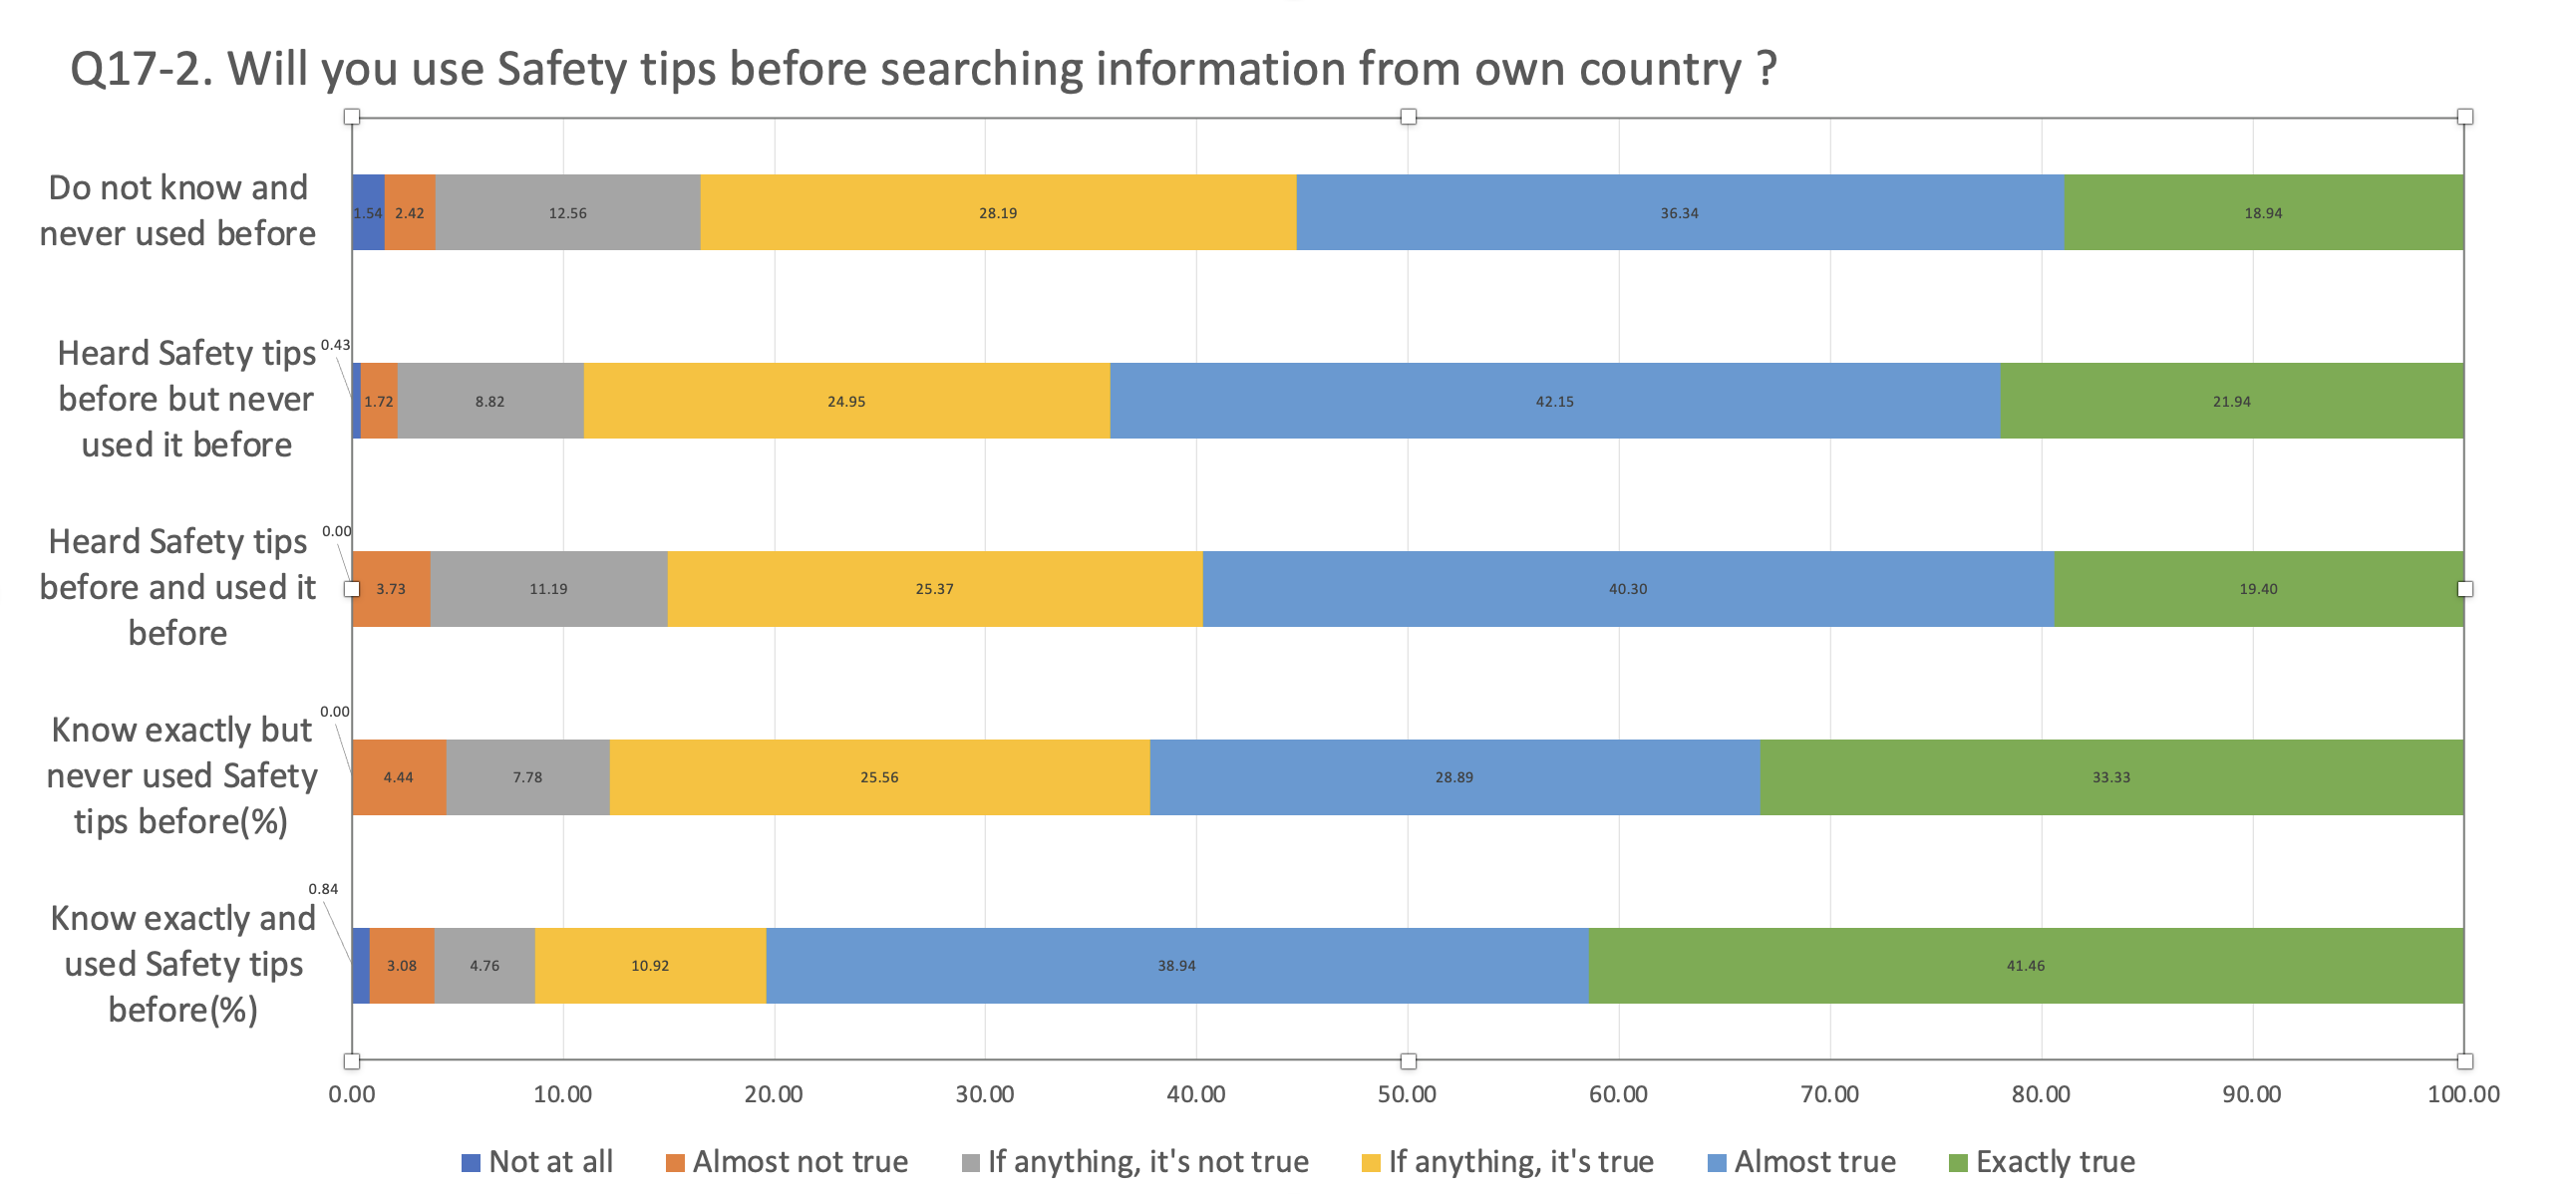
\includegraphics[width=0.8\linewidth]{Figure/Figure20.jpg}
  \centering
  \caption[5 groups of respondents' survey result of Q17\_2]{5 groups of respondents' survey result of Q17\_2(Will you use Safety Tips before searching information from your own country ?)}
  \label{fig20}
\end{figure*}

For Q17\_3, do the respondents think Safety Tips could be useful during the evacuation, the result is shown in Figure~\ref{fig21}. we can find that respondents that know exactly and used Safety Tips before and respondents who heard Safety Tips before but never used Safety Tips before could be more likely to believe Safety Tips could be useful during evacuation. Respondents that do not know and never used before, respondents who heard and used Safety Tips before, respondents who know exactly but never used Safety Tips before could be more likely to show lower usefulness of Safety Tips. 

\begin{figure*}[h]
  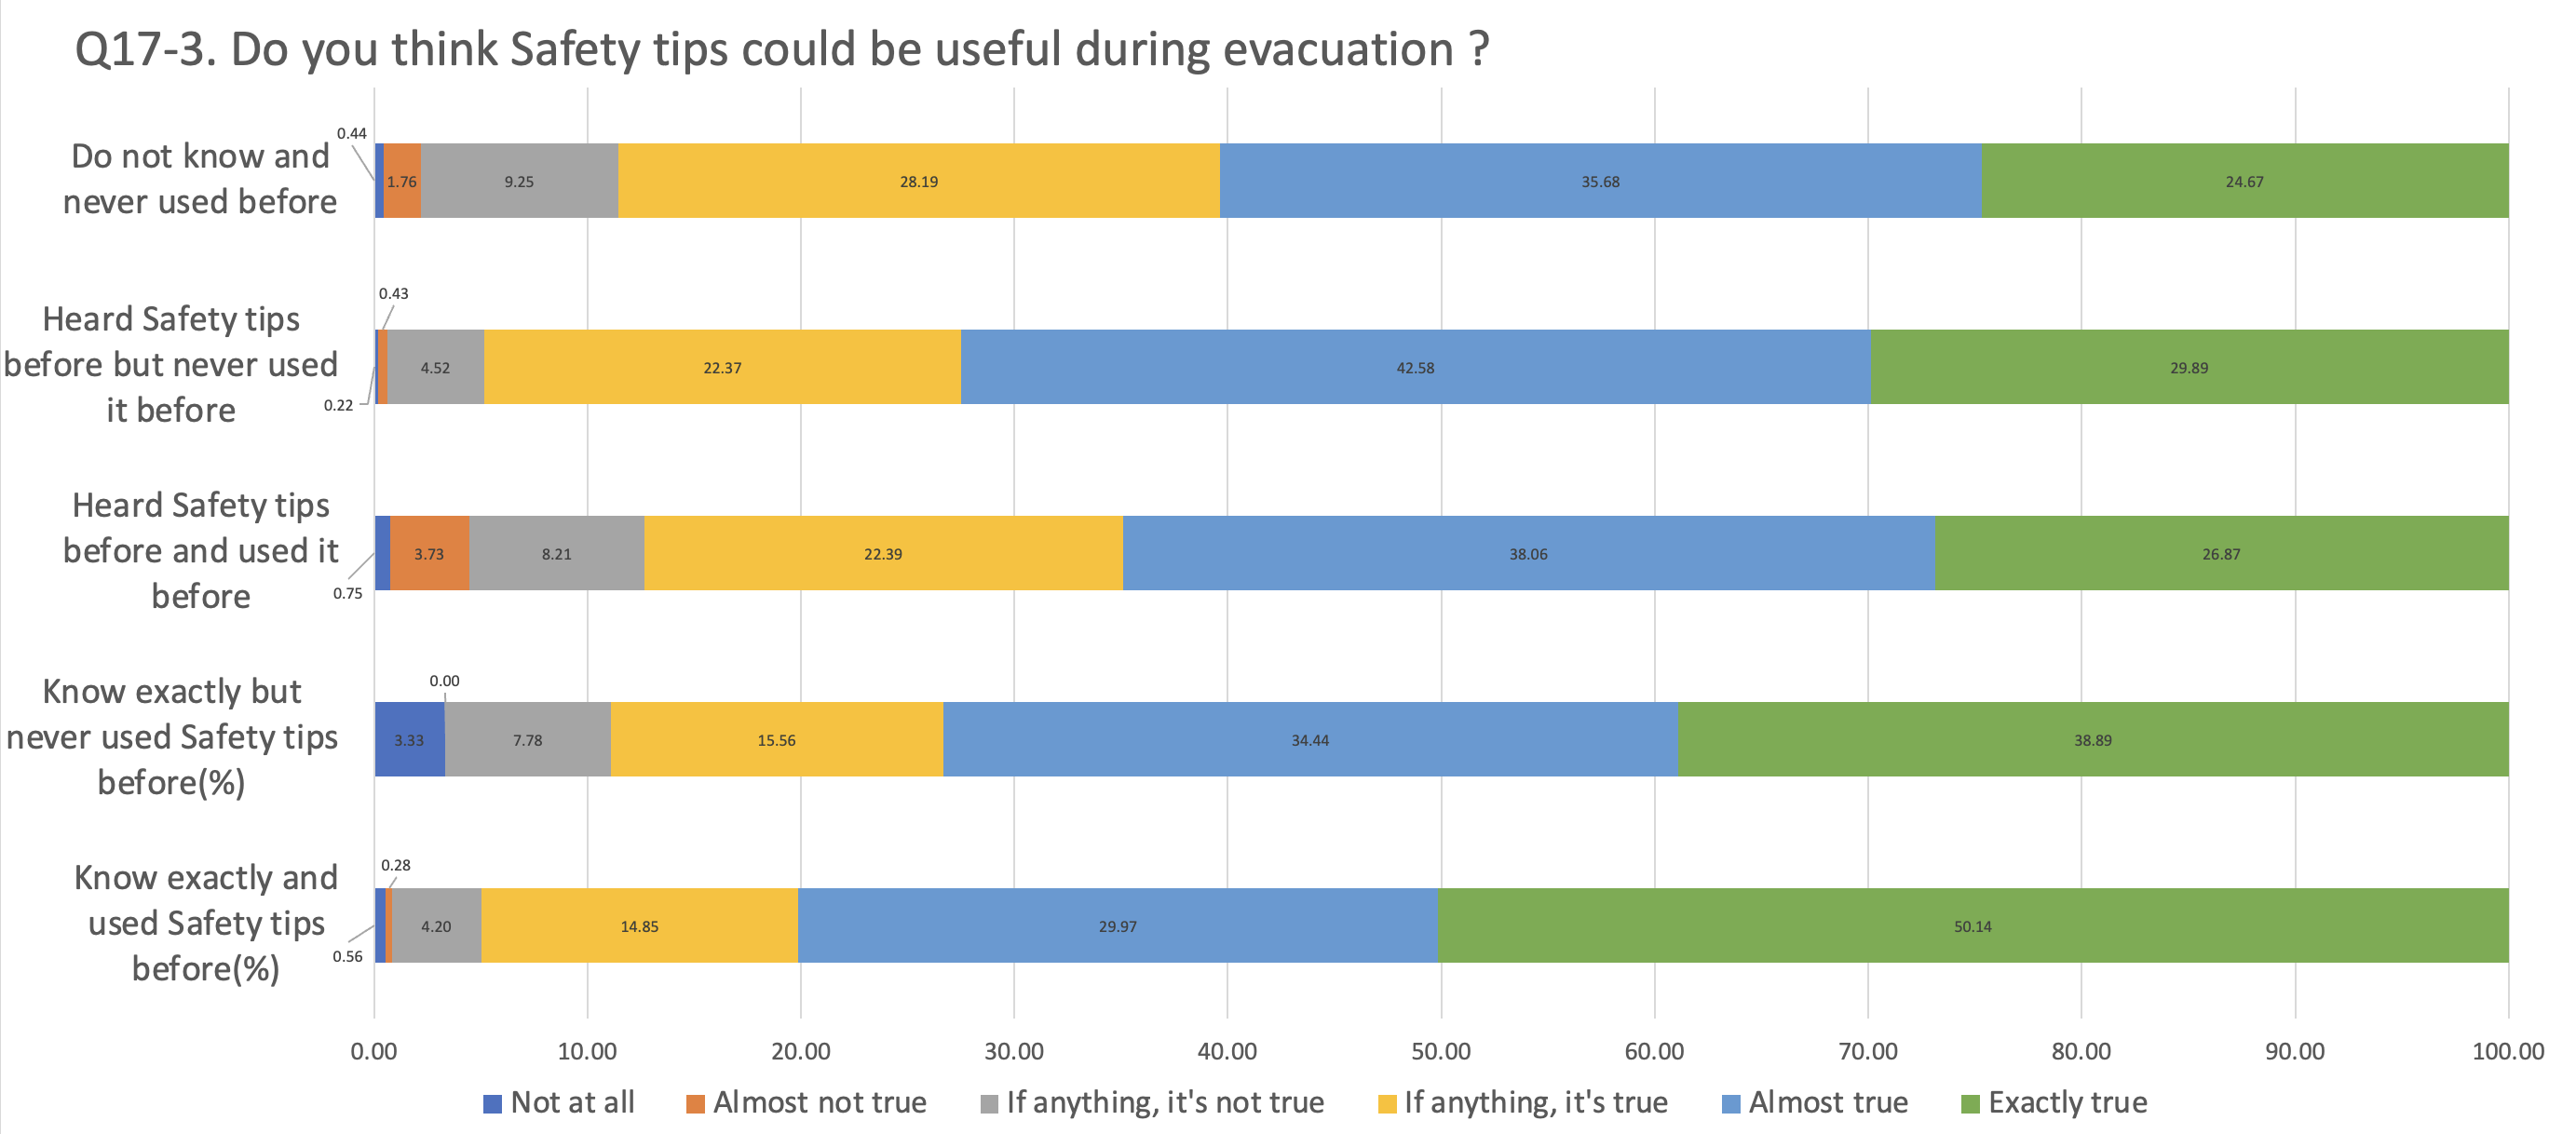
\includegraphics[width=0.8\linewidth]{Figure/Figure21.jpg}
  \centering
  \caption[5 groups of respondents' survey result of Q17\_3]{5 groups of respondents' survey result of Q17\_3(Do you think Safety Tips could be useful during evacuation ?)}
  \label{fig21}
\end{figure*}

For Q17\_4, will the respondents use Safety Tips in the future, the result shows in Figure~\ref{fig22}. we can find that respondents that know exactly and used Safety Tips before and respondents who heard but never used Safety Tips before have shown higher usage possibly Safety Tips in the future. Respondents that do not know and never used before, respondents who heard and used Safety Tips before, respondents who know exactly but never used Safety Tips before have shown relatively lower usage possibility.

\begin{figure*}[h]
  \includegraphics[width=0.8\linewidth]{Figure/Figure22.jpg}
  \centering
  \caption[5 groups of respondents' survey result of Q17\_4]{5 groups of respondents' survey result of Q17\_4(Will you use Safety Tips in the future ?)}
  \label{fig22}
\end{figure*}

From the above results, we can conclude that respondents that know exactly and used Safety Tips before could show higher trust and higher priority of use on Safety Tips, also they are more likely to believe Safety Tips can be useful during the evacuation, and they will use it in the future. And, respondents that heard but never used  Safety Tips before have shown better attitudes on Safety Tips rather than respondents who do not know and never used  Safety Tips before, respondents who heard and used Safety Tips before, respondents who know exactly but never used it Safety Tips before.

The results of the grouping indicate that 80\% of those who clearly know Safety Tips have actually used Safety Tips before. For those who had only heard of Safety Tips, only 22\% of the respondents had used Safety Tips before. Comparing the two sets of data, it is clear that the usage rate has decreased significantly. This shows that people who have a more detailed awareness of Safety Tips are more likely to use this application, so if we want to increase the usage of Safety Tips, it would be helpful to increase foreign visitors' awareness of this application.
\cleardoublepage
%%%%%%%%%%%%%%%%%%%
\section{Results for Objective 2 }
Table~\ref{table27} shows the results of the statistical description with the maximum value, minimum value, mean, and standard deviation for each variable.

\begin{table}[h]
  \caption[Statistical Description]{Statistical Description (N=491)}
  \label{table27}
  \centering
  \begin{tabular}{l|cccc}
 \hline
\multicolumn{1}{c|}{Variable} & Min value  & Max value & Mean & Standard Deviation \\
 \hline
Country	& 2&6&4.32&1.30\\
gender&1&2&1.48&0.50\\
age&2&7&4.37&1.26\\
Visit\_country&1&10&4.39&2.61\\
Visit\_Japan&1&11&4.99&2.92\\
Japanese\_Level&1&4&2.59&0.77\\
Q1&1&6&4.94&1.02\\
Q2&1&6&4.95&1.01\\
Q3&1&6&5.08&0.99\\
Q4&1&6&4.55&1.03\\
Q5&1&6&3.83&1.41\\
Q6\_1\_earthquake&0&12&4.95&3.74\\
Q6\_2\_tsunami&0&12&4.53&3.33\\
Q6\_3\_typhoon&0&12&4.6&3.43\\
Q6\_4\_fire&0&12&5.01&4.06\\
Q7\_1\_earthquake&0&4&1.66&1.60\\
Q7\_2\_tsunami&0&4&0.80&1.27\\
Q7\_3\_typhoon&0&4&0.72&1.29\\
Q7\_4\_fire&0&4&1.48&1.61\\
Q8\_experience\_earthquake&1&8&3.15& 1.87\\
Q9&1&6&4.88&0.97\\
Q10	&1&6&5.01&0.95\\
Q15 Safetytips&2&3&2.73&0.45\\
Q16 Safetytips\_use&1&1&1&0\\
Q17 Safetytips\_trust\_1&1&6&4.8&1.31\\
Q17 Safetytips\_trust\_2&1&6&4.95&1.08\\
Q17 Safetytips\_trust\_3&1&6&5.10&1.01\\
Q17 Safetytips\_trust\_4&1&6&5.11&1.02\\
 \hline
  \end{tabular}
\end{table}

For some group-based data, the frequency descriptions of these variables are shown in the following. \crefrange{table28a}{table28f} is the frequency description of Item 1, including Country, Gender, Age, number of visited countries, number of visited Japan, Japanese Level. Table~\ref{table28g} is the frequency description of Item 3, that is the severity of the earthquake experience.

\begin{table}[h]
  \caption[Frequency Description of Country]{Frequency Description of Country (N=491)}
  \label{table28a}
  \centering
  \begin{tabular}{l|cc}
 \hline
\multicolumn{1}{c|}{Category}&Number&Rate\\
 \hline
China&78&15.90\%\\
South Korea&42&8.60\%\\
Thailand&105&21.40\%\\
Indonesia&179&36.50\%\\
the UK&87&17.70\%\\
 \hline
  \end{tabular}
\end{table}

\begin{table}[h]
  \caption[Frequency Description of Gender]{Frequency Description of Gender (N=491)}
  \label{table28b}
  \centering
  \begin{tabular}{l|cc}
 \hline
\multicolumn{1}{c|}{Category}&Number&Rate\\
 \hline
Male   & 253 & 51.50\% \\
Female & 238 & 48.50\% \\
 \hline
  \end{tabular}
\end{table}

\begin{table}[h]
  \caption[Frequency Description of Age]{Frequency Description of Age (N=491)}
  \label{table28c}
  \centering
  \begin{tabular}{l|cc}
 \hline
\multicolumn{1}{c|}{Category}&Number&Rate\\
 \hline
Age 16-19   & 13  & 2.60\%  \\
Age 20-29   & 136 & 27.70\% \\
Age 30-39   & 126 & 25.70\% \\
Age 40-49   & 113 & 23\%    \\
Age 50-59   & 77  & 15.70\% \\
Age 60-69   & 26  & 5.30\%  \\
Age over 70 & 0   & 0\% \\
 \hline
  \end{tabular}
\end{table}

\begin{table}[h]
  \caption[Frequency Description of number of visited country ]{Frequency Description of number of visited country (N=491)}
  \label{table28d}
  \centering
  \begin{tabular}{l|cc}
 \hline
\multicolumn{1}{c|}{Category}&Number&Rate\\
 \hline
0 time        & 0                    & 0\%                  \\
1 time        & 73                   & 14.90\%              \\
2 times       & 63                   & 12.80\%              \\
3 to 4 times  & 152                  & 31\%                 \\
5 to 6 times  & 95                   & 19.30\%              \\
7 to 9 times  & 99                   & 20.20\%              \\
Over 10 times & 9                    & 1.80\%               \\
 \hline
  \end{tabular}
\end{table}

\begin{table}[h]
  \caption[Frequency Description of number of visited Japan]{Frequency Description of number of visited Japan (N=491)}
  \label{table28e}
  \centering
  \begin{tabular}{l|cc}
 \hline
\multicolumn{1}{c|}{Category}&Number&Rate\\
 \hline
0 time        & 0   & 0\%     \\
1 time        & 47  & 9.60\%  \\
2 times       & 65  & 13.20\% \\
3 to 4 times  & 147 & 29.90\% \\
5 to 6 times  & 85  & 17.30\% \\
7 to 9 times  & 81  & 16.50\% \\
Over 10 times & 66  & 13.40\% \\
 \hline
  \end{tabular}
\end{table}

\begin{table}[h]
  \caption[Frequency Description of Japanese Level]{Frequency Description of Japanese Level (N=491)}
  \label{table28f}
  \centering
  \begin{tabular}{l|cc}
 \hline
\multicolumn{1}{c|}{Category}&Number&Rate\\
 \hline
Cannot understand                    & 25  & 5.10\%  \\
Basic        & 214 & 43.60\% \\
Intermediate & 190 & 38.70\% \\
Up level     & 62  & 12.60\% \\
 \hline
  \end{tabular}
\end{table}

\begin{table}[h]
  \caption[Frequency Description of severity of the earthquake experienced]{Frequency Description of severity of the earthquake experienced (N=491)}
  \label{table28g}
  \centering
  \begin{tabular}{l|cc}
 \hline
\multicolumn{1}{c|}{Category}&Number&Rate\\
 \hline
MMI intensity 5 or less / intensity 3 or less & 110 & 22.40\% \\
MMI intensity 6 / intensity 4                 & 90  & 18.30\% \\
MMI intensity 7 / intensity 5 weak            & 119 & 24.20\% \\
MMI intensity 8 / intensity 5 strong          & 80  & 16.30\% \\
MMI intensity 9 / intensity 6 weak            & 30  & 6.10\%  \\
MMI intensity 10 / intensity 6 strong                                 & 18  & 3.70\%  \\
MMI intensity 11 to 12 / intensity 7                                  & 30  & 6.10\%  \\
no earthquake experience                                              & 14  & 2.90\%  \\
 \hline
  \end{tabular}
\end{table}







%\iffalse
\begin{table}[h]
\caption{T-test result: Gender with attitudes towards Safety Tips.}
\label{table24}
\centering
\begin{tabular}{|c|c|c|c|c|}
\hline
& \begin{tabular}{c}Male($=$1)\\(n=750)\end{tabular} & \begin{tabular}{c}Female($=$2)\\(n=750)\end{tabular} & t & p \\
\hline
Q17 SafetyTips\_trust\_1 & 4.54$\pm$1.22 & 4.59$\pm$1.21 & $-$0.848 & 0.396 \\
\hline
Q17 SafetyTips\_trust\_2 & 4.74$\pm$1.09 & 4.75$\pm$1.06 & $-$0.120 & 0.904 \\
\hline
Q17 SafetyTips\_trust\_3 & 4.86$\pm$1.03 & 5.00$\pm$0.96 & $-$2.643 & 0.008 \\
\hline
Q17 SafetyTips\_trust\_4 & 4.88$\pm$1.09 & 5.94$\pm$1.07 & $-$0.933 & 0.351 \\
\hline
\end{tabular}
\end{table}

\begin{table}[h]
\caption{T-test result: Age with attitudes towards Safety Tips.}
\label{table25}
\centering
\begin{tabular}{|c|c|c|c|c|}
\hline
& \begin{tabular}{c}Age under 39($<$4)\\(n=370)\end{tabular} & \begin{tabular}{c}Age over 40($>=$4)\\(n=1130)\end{tabular} & t & p \\
\hline
Q17 SafetyTips\_trust\_1 & 4.34$\pm$1.30 & 4.64$\pm$1.18 & 4.015 & 0.000 \\
\hline
Q17 SafetyTips\_trust\_2 & 4.57$\pm$1.14 & 4.80$\pm$1.05 & 3.361 & 0.001 \\
\hline
Q17 SafetyTips\_trust\_3 & 4.78$\pm$1.05 & 4.98$\pm$0.98 & 3.204 & 0.001 \\
\hline
Q17 SafetyTips\_trust\_4 & 4.78$\pm$1.38 & 4.95$\pm$1.06& 2.555 & 0.011 \\
\hline
\end{tabular}
\end{table}
%\fi

\begin{table}[h]
\caption{T-test result: Japanese Level with attitudes towards Safety Tips.}
\label{table26}
\centering
\begin{tabular}{|c|c|c|c|c|}
\hline
& \begin{tabular}{c}can understand\\($>=$3)(n=453)\end{tabular} & \begin{tabular}{c}can not understand\\($<$3)(n=1047)\end{tabular} & t & p \\
\hline
Q17 SafetyTips\_trust\_1 & 4.73$\pm$1.22 & 4.49$\pm$1.21 & 3.455 & 0.001 \\
\hline
Q17 SafetyTips\_trust\_2 & 4.83$\pm$1.08& 4.71$\pm$1.07 & 1.977 & 0.048 \\
\hline
Q17 SafetyTips\_trust\_3 & 4.99$\pm$1.01 & 4.90 $\pm$0.99 & 1.537 & 0.125 \\
\hline
Q17 SafetyTips\_trust\_4 & 4.99$\pm$1.05 & 4.88$\pm$1.09 & 1.841 & 0.066 \\
\hline
\end{tabular}
\end{table}


\begin{table}[h]
  \caption{T-test result: past awareness of Safety Tips with attitudes towards Safety Tips. }
  \label{table6}
  \centering
  \begin{tabular}{|c|c|c|c|c|}
  \hline
     & \begin{tabular}{c}Q15 Safety Tips:\\don't know ($=$1)\\(n=454)\end{tabular} & \begin{tabular}{c}Q15 Safety Tips:\\know($>=$2)\\(n=1046)\end{tabular} & t & p \\
  \hline
   Q17 SafetyTips\_trust\_1 & 4.35$\pm$1.19 & 4.66$\pm$1.22 & 4.49 & 0.000 \\
  \hline
   Q17 SafetyTips\_trust\_2 & 4.52$\pm$1.10 & 4.84$\pm$1.05 & 5.18 & 0.000 \\
  \hline
   Q17 SafetyTips\_trust\_3 & 4.71$\pm$1.02 & 5.03$\pm$0.97 & 5.61 & 0.000 \\
  \hline
   Q17 SafetyTips\_trust\_4 & 4.59$\pm$1.15 & 5.05$\pm$1.02 & 7.43 & 0.000 \\
  \hline
  \end{tabular}
\end{table}

%%%%%%%%%%%%%%%%%%%
%\iffalse
\begin{table}[h]
  \caption{T-test result: using experience of Safety Tips with attitudes towards Safety Tips.}
  \label{table7}
  \centering
  \begin{tabular}{|c|c|c|c|c|}
  \hline
     & \begin{tabular}{c}Q16 SafetyTips\_use:\\used before($=$1)\\(n=491)\end{tabular} & \begin{tabular}{c}Q16 SafetyTips\_use:\\never used before($=$0)\\(n=555)\end{tabular} & t & p \\
  \hline
   Q17 SafetyTips\_trust\_1 & 4.80$\pm$1.31 & 4.53$\pm$1.12 & $-$3.49 & 0.001 \\
  \hline
   Q17 SafetyTips\_trust\_2 & 4.95$\pm$1.08 & 4.74$\pm$1.01 & $-$3.38 & 0.001 \\
  \hline
   Q17 SafetyTips\_trust\_3 & 5.10$\pm$1.01 & 4.96$\pm$0.94 & $-$2.34 & 0.019 \\
  \hline
   Q17 SafetyTips\_trust\_4 & 5.11$\pm$1.02 & 5.00$\pm$1.01 & $-$1.72 & 0.086 \\
  \hline
  \end{tabular}
\end{table}
%\fi






\subsection{Model 1}

We constructed the SEM model 1 shown in Figure~\ref{fig23} based on the previous hypotheses in Chapter 4.2 to explore the relationship between the latent variables of 'Training Experience', 'Consciousness', 'Knowledge', and 'Attitudes toward Safety Tips'. The five manifest variables of 'Consciousness' (the responses of Q1-Q5), the two manifest variables of 'Knowledge' (the responses of Q9-Q10), and the four manifest variables of  'Attitudes toward Safety Tips' (the responses of Q17\_1-Q17\_4) are all continuum selections, so it is necessary to test the score reliability coefficient. When multiple questions are asked about a characteristic and the sum of the responses (scale scores) is used as the characteristic scale, the reliability coefficient that assesses whether each questionnaire item (variable) measures the same concept or object as a whole (internal consistency) is called Cronbach's alpha. Cronbach's alpha is calculated by the following formula. 
\begin{equation}
\alpha = \frac{m}{m-1} \left(1 - \frac{\displaystyle \sum_{i = 1}^m{{\sigma_i}^2}}{{\sigma_x}^2} \right)
\end{equation}
$m$ means the number of items in the question; ${\sigma_i}^2$ means the variance of each question item; ${\sigma_x}^2$ means the variance of the total scale score for each question item. Cronbach's alpha has a value between 0 and 1, and the closer the value is to 1, the more reliable it is. The evaluation of Cronbach's alpha, as shown in Figure~\ref{fig24}, was suggested by George and Mallery~\cite{ref1}. Cronbach's alpha  Cronbach's alpha of 0.9 indicates excellent internal consistency, 0.8 indicates good, 0.7 indicates acceptable, 0.6 indicates poor, and 0.5 unacceptable. The results of the alpha reliability coefficient test are shown in Table~\ref{table8}, the Cronbach's alpha values of Q1-Q5 is 0.869, for Q9-Q10 is 0.927, and for Q7\_1-Q17\_4 is 0.871. The total Cronbach's alpha value for all the above variables is 0.935. We can find that the Cronbach's alpha value of any one of them is satisfying the evaluation criteria.

%%%%%%%%%%%%%%%%%%%
%\iffalse
\begin{figure*}[h]
  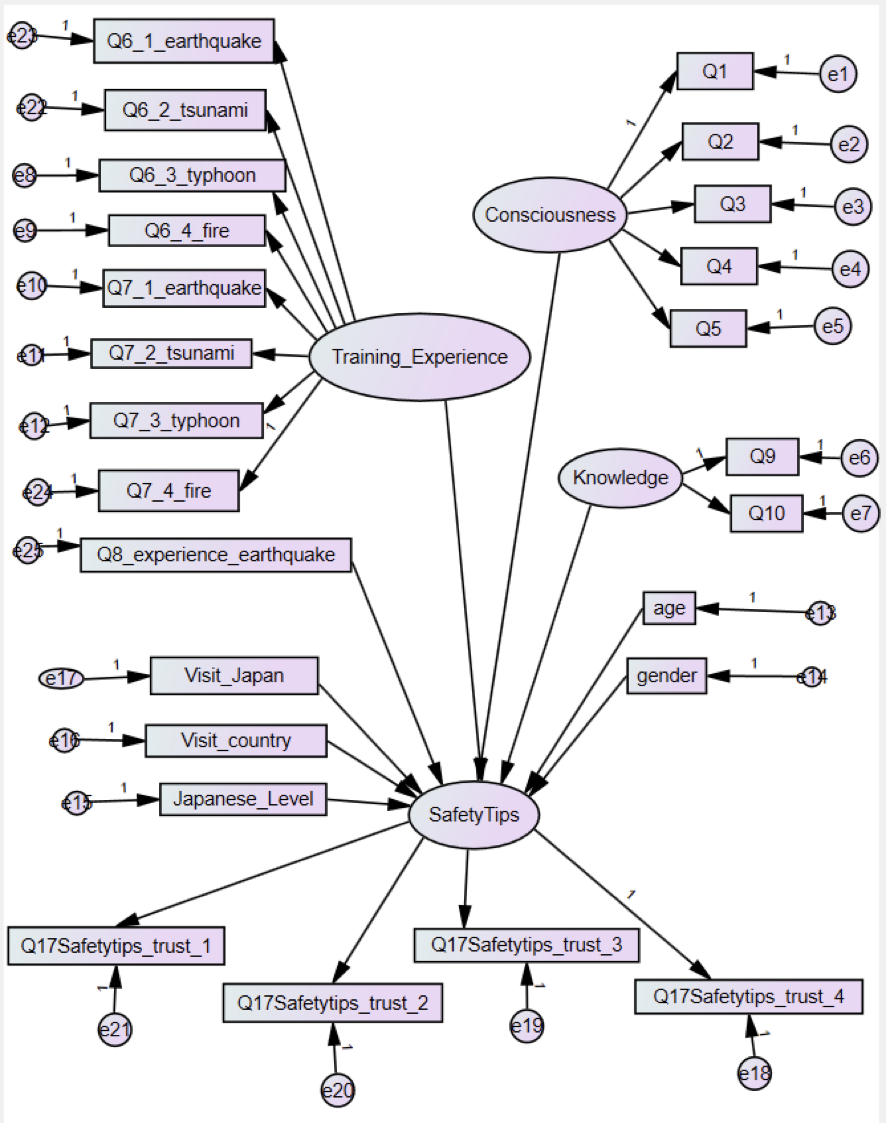
\includegraphics[width=0.5\linewidth]{Figure/Figure23.jpg}
  \centering
  \caption{SEM model 1}
  \label{fig23}
\end{figure*}

\begin{figure*}[h]
  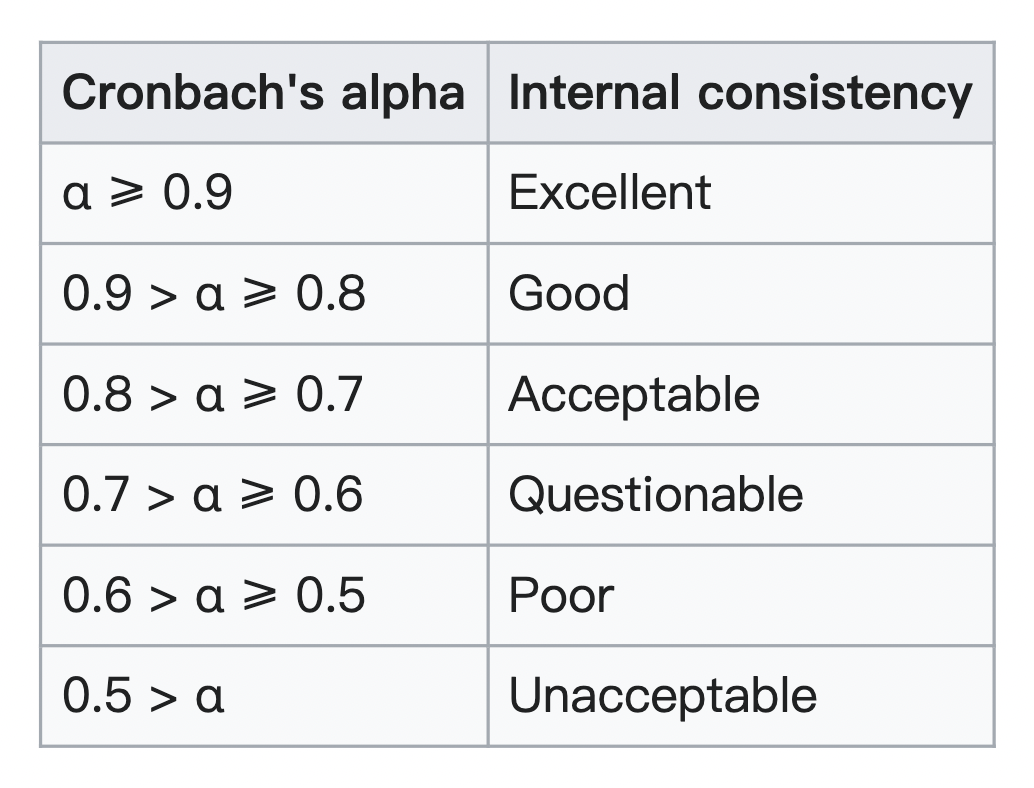
\includegraphics[width=0.5\linewidth]{Figure/Figure24.jpg}
  \centering
  \caption{Evaluation of score reliability coefficient test}
  \label{fig24}
\end{figure*}


\begin{table}[h]
  \caption{Result of score reliability coefficient test}
  \label{table8}
  \centering
  \begin{tabular}{|c|c|c|}
  \hline
          & Cronbach's alpha value & Objects \\
 \hline 
  Q1 to Q5 & 0.869 & 20 \\
 \hline
  Q9 and Q10 & 0.927 & 15 \\
 \hline 
  Q17 & 0.871 & 4 \\
 \hline
  All & 0.935 & 39 \\
 \hline
  \end{tabular}
\end{table}
%\fi

The result of Regression Weights for Model 1 shows in Table~\ref{table9} and the result of Standard Regression Weights for Model 1 is shown in Table~\ref{table10}. From the result, we can find that 'Consciousness', 'Knowledge', 'Earthquake experience', 'Japanese level' could show significant relationships with respondents' attitude on Safety Tips. While, 'Age', 'Gender', 'Visit Japan', 'Visit country' don't show significant relationships with respondents' attitudes toward Safety Tips. Currently, 'training experience' also doesn't have a significant relationship with respondents' attitude on Safety Tips. Because 'training experience' is a potential variable in our original hypothesis, I'd like to go deeper into the relationship with some improvements. We can get a better estimate of the true correlation by disattenuated the variables, according to D. Streiner~\cite{Streiner2006BuildingAB}. Two things happen when we add extra variables. First, the model's ability to account for more variance grows. Each new variable, on the other hand, enhances the error variance. As a result, the previous model will struggle to accommodate the additional data, which is a consequence of adding more variables to the model. We can see that Q6 1/2/3/4 and Q7 1/2/3/4 both have a significant relationship with 'Training Experience' based on the results of Table~\ref{table9} Regression Weights. However, the estimated value of Q7 1/2/3/4 is much lower than the estimated value of Q6 1/2/3/4, as seen in Table~\ref{table10} Standardized Regression Weights. This means that Q6 is better than Q7 at expressing the latent variable 'Training Experience'. The two manifest variables are similar in structure: Q6 is for the experience of a given event, and the total score is used as data, whereas Q7 is for the number of times. Because the similarity of the two variables causes a significant amount of inaccuracy in the expression of the latent variable, we'll delete Q7 and keep only Q6 as the manifest variable to express 'Training experience' as a way to improve the model. Furthermore, we believe there may have a correlation relationship between 'Training Experience', 'Consciousness', and 'Knowledge'. Therefore adding the correlation between these three latent variables is another way to improve the model. Finally, since the result shows that 'Age', 'Gender', 'Visit Japan', and 'Visit Country' have no significant relationship with 'Attitude toward Safety Tips', deleting these four variables could be also a way to improve the model. Based on the above three improvement ideas shown on the left side of  Figure~\ref{fig25}, we construct Model 2 shown on the right side of Figure~\ref{fig25}.

%%%%%%%%%%%%%%%%%%%
%\iffalse
\begin{figure*}[h]
  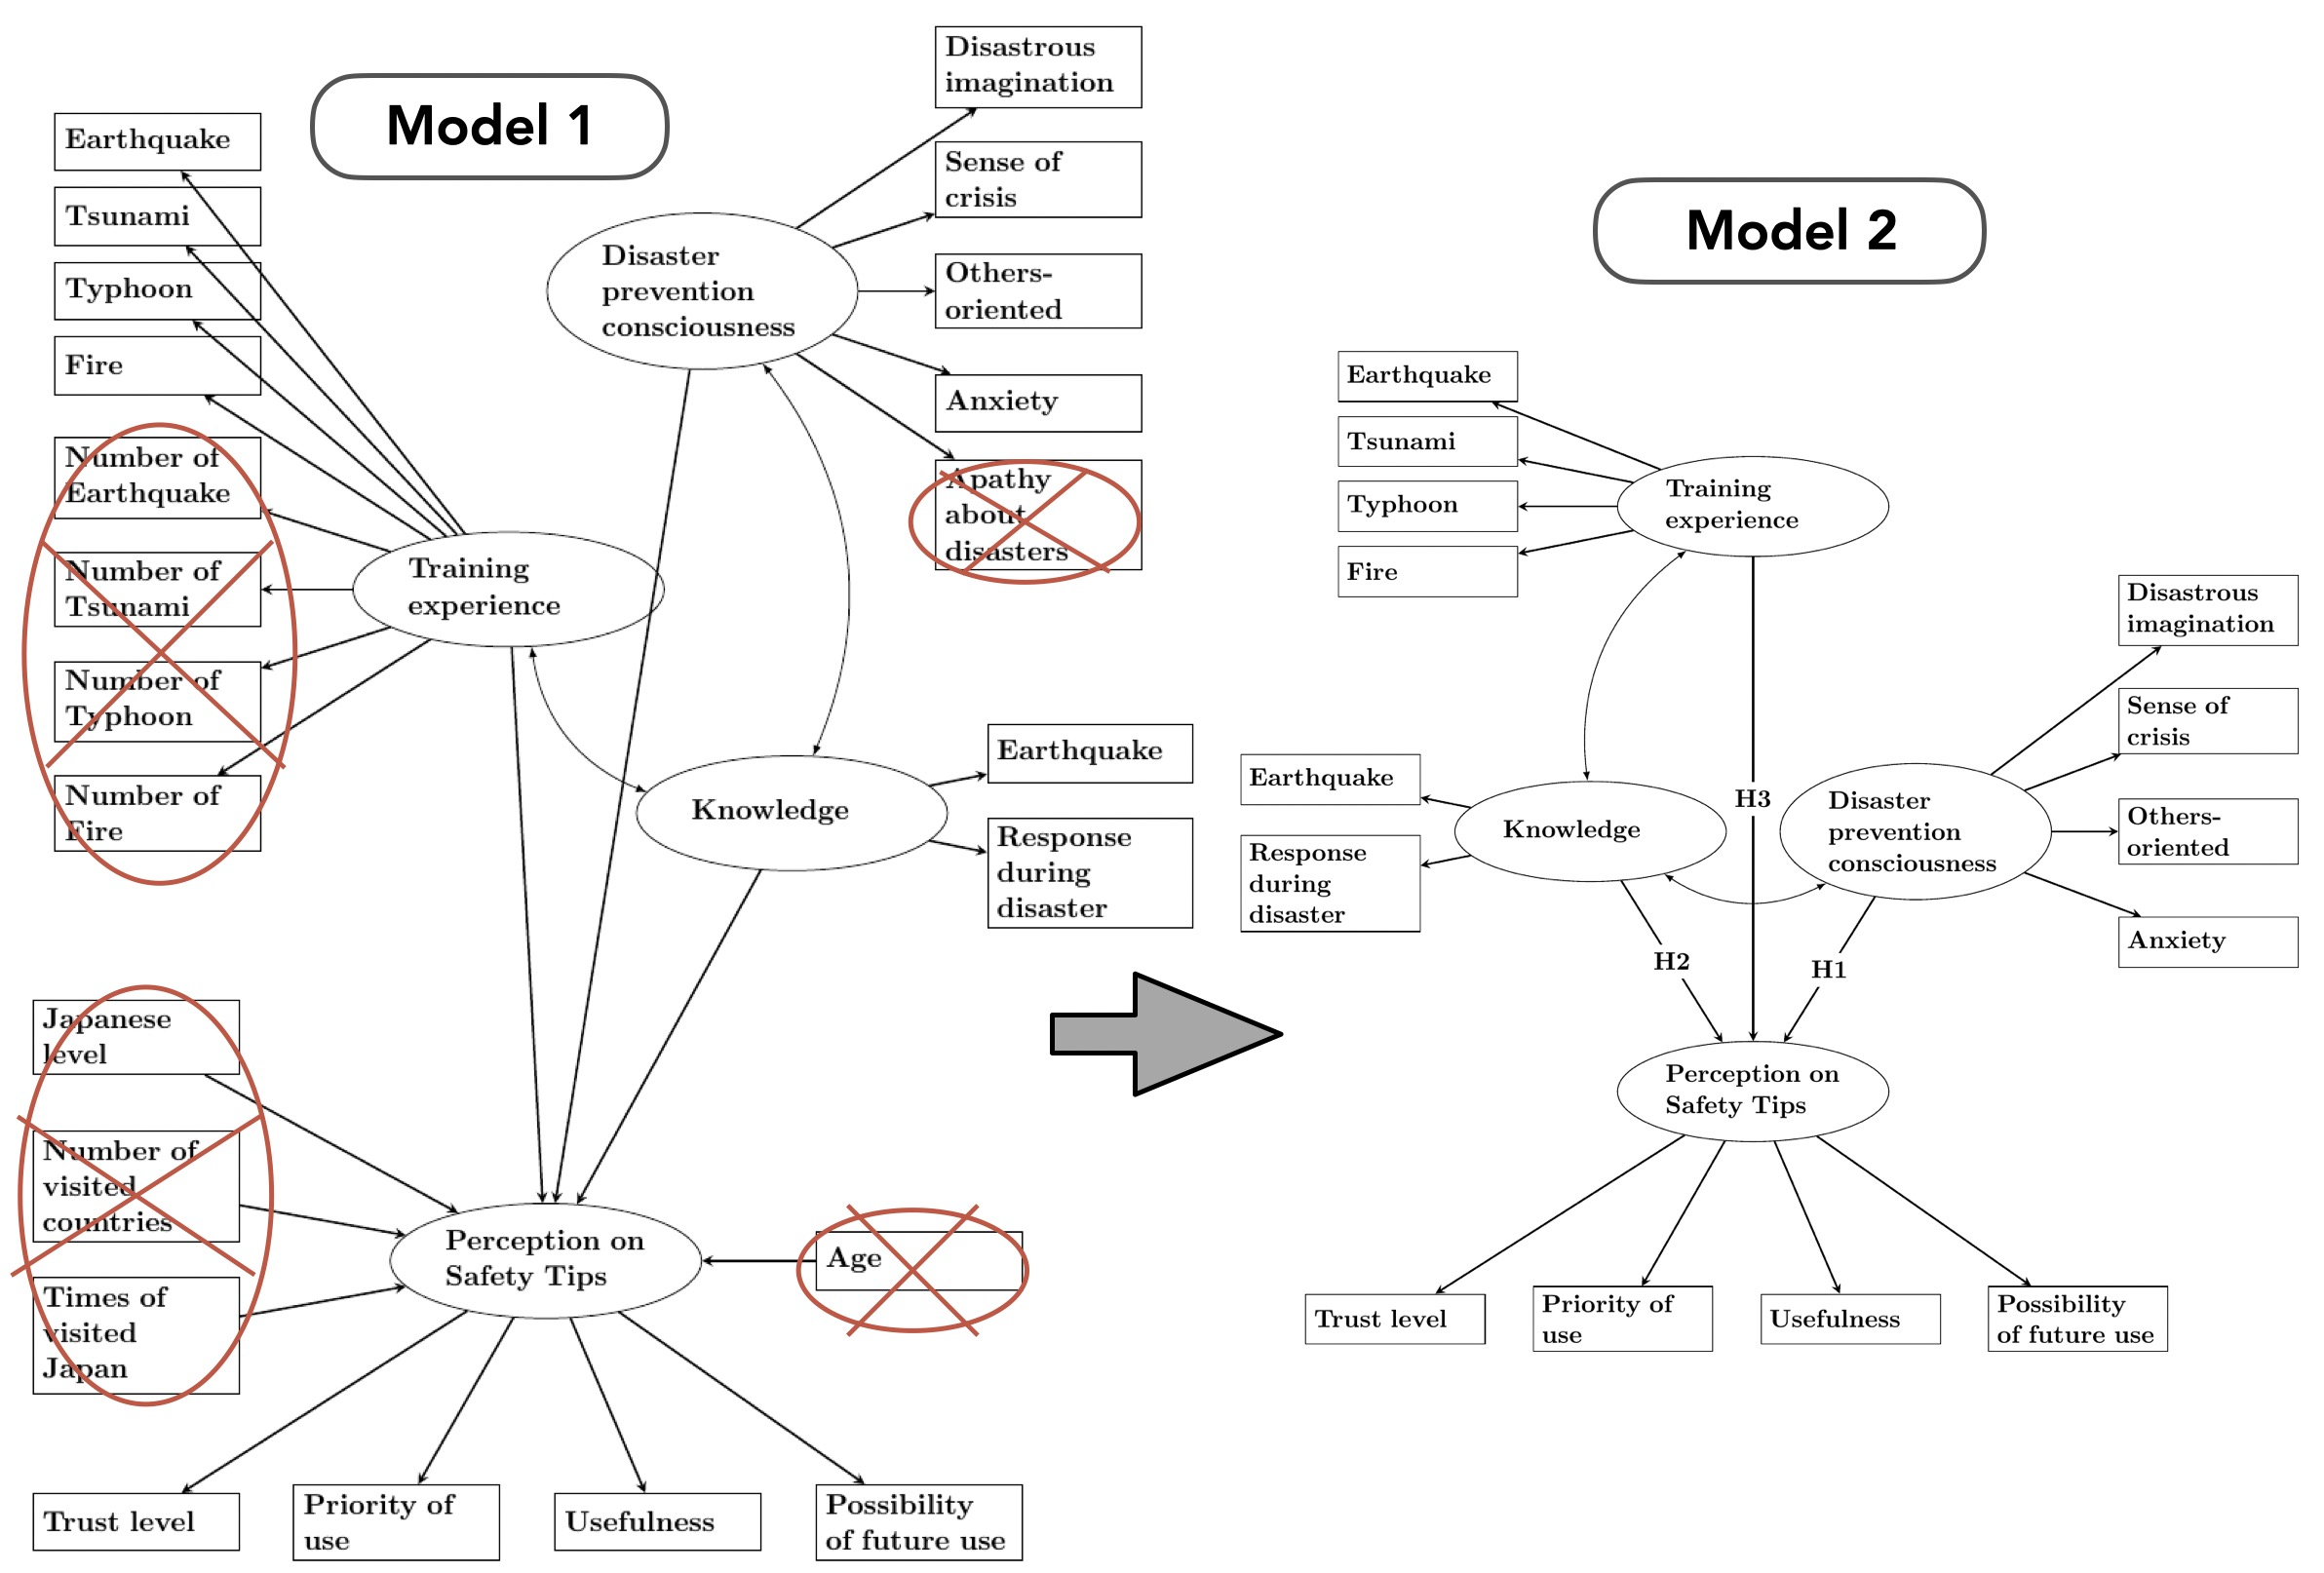
\includegraphics[width=\linewidth]{Figure/Figure25.png}
  \centering
  \caption[SEM model 2]{Left side: the diagram contains the improvement points made based on Model 1,Right side: Model 2}
  \label{fig25}
\end{figure*}


\begin{table}[h]
  \caption{Regression Weights of Model 1}
  \label{table9}
  \centering
  \begin{tabular}{|l|c|l|c|c|}
 \hline
 \multicolumn{3}{|c|}{Regression Weights} & Estimate & p \\
 \hline
  Safety Tips & $\longleftarrow$ & Age & 0.036 & 0.007 \\ 
  Safety Tips & $\longleftarrow$ & Gender &0.065 & 0.053 \\
  Safety Tips & $\longleftarrow$ & Training Experience & $-$0.075 & 0.003 \\
  Safety Tips & $\longleftarrow$ & Consciousness & 0.194 & *** \\
  Safety Tips & $\longleftarrow$ & Knowledge & 1.448 & *** \\
  Safety Tips & $\longleftarrow$ & Visit Country & 0.002 & 0.803 \\
  Safety Tips & $\longleftarrow$ & Japanese Level & $-$0.095 & *** \\
  Safety Tips & $\longleftarrow$ & Visit Japan & 0.006 & 0.377 \\
  Safety Tips & $\longleftarrow$ & Q8\_experience\_earthquake & $-$0.225 & *** \\
  Q1              & $\longleftarrow$ & Consciousness & 1.000 &  \\
  Q2              & $\longleftarrow$ & Consciousness & 0.790 & *** \\
  Q3              & $\longleftarrow$ & Consciousness & 0.868 & *** \\
  Q4              & $\longleftarrow$ & Consciousness & 0.677 & *** \\
  Q5              & $\longleftarrow$ & Consciousness & 0.158 & *** \\
  Q6\_1\_earthquake & $\longleftarrow$ & Training Experience & 3.677 & *** \\
  Q6\_2\_tsunami & $\longleftarrow$ & Training Experience & 3.341 & *** \\
  Q6\_3\_typhoon & $\longleftarrow$ & Training Experience & 3.576 & *** \\
  Q6\_4\_fire & $\longleftarrow$ & Training Experience & 3.672 & *** \\
  Q7\_1\_earthquake & $\longleftarrow$ & Training Experience & 0.949 & *** \\
  Q7\_2\_tsunami & $\longleftarrow$ & Training Experience & 0.614 & *** \\
  Q7\_3\_typhoon & $\longleftarrow$ & Training Experience & 0.725 & *** \\
  Q7\_4\_fire & $\longleftarrow$ & Training Experience & 1.000 & \\
  Q9             & $\longleftarrow$ & Knowledge & 1.000 & \\
  Q10           & $\longleftarrow$ & Knowledge & 1.028 & *** \\
  Q17 SafetyTips\_trust\_1 & $\longleftarrow$ & Safety Tips & 1.118 & *** \\
  Q17 SafetyTips\_trust\_2 & $\longleftarrow$ & Safety Tips & 1.000 & \\
  Q17 SafetyTips\_trust\_3 & $\longleftarrow$ & Safety Tips & 1.012 & *** \\
  Q17 SafetyTips\_trust\_4 & $\longleftarrow$ & Safety Tips & 1.000 & \\
 \hline
  \end{tabular}
\end{table}

\begin{table}[h]
  \caption{Standardized Regression Weights of Model 1 }
  \label{table10}
  \centering
  \begin{tabular}{|l|c|l|c|}
 \hline
 \multicolumn{3}{|c|}{Standardized Regression Weights} & Estimate \\
 \hline
  Safety Tips & $\longleftarrow$ & Age & 0.057 \\ 
  Safety Tips & $\longleftarrow$ & Gender &0.040 \\
  Safety Tips & $\longleftarrow$ & Training Experience & $-$0.067 \\
  Safety Tips & $\longleftarrow$ & Consciousness & 0.191 \\
  Safety Tips & $\longleftarrow$ & Knowledge & 0.967 \\
  Safety Tips & $\longleftarrow$ & Visit Country & 0.005 \\
  Safety Tips & $\longleftarrow$ & Japanese Level & $-$0.094 \\
  Safety Tips & $\longleftarrow$ & Visit Japan & 0.018 \\
  Safety Tips & $\longleftarrow$ & Q8\_experience\_earthquake & $-$0.102 \\
  Q1              & $\longleftarrow$ & Consciousness & 0.760\\
  Q2              & $\longleftarrow$ & Consciousness & 0.706 \\
  Q3              & $\longleftarrow$ & Consciousness & 0.703\\
  Q4              & $\longleftarrow$ & Consciousness & 0.540 \\
  Q5              & $\longleftarrow$ & Consciousness & 0.112 \\
  Q6\_1\_earthquake & $\longleftarrow$ & Training Experience & 0.785 \\
  Q6\_2\_tsunami & $\longleftarrow$ & Training Experience & 0.838 \\
  Q6\_3\_typhoon & $\longleftarrow$ & Training Experience & 0.862 \\
  Q6\_4\_fire & $\longleftarrow$ & Training Experience & 0.706 \\
  Q7\_1\_earthquake & $\longleftarrow$ & Training Experience & 0.484 \\
  Q7\_2\_tsunami & $\longleftarrow$ & Training Experience & 0.473 \\
  Q7\_3\_typhoon & $\longleftarrow$ & Training Experience & 0.521 \\
  Q7\_4\_fire & $\longleftarrow$ & Training Experience & 0.465\\
  Q9             & $\longleftarrow$ & Knowledge & 0.512\\
  Q10           & $\longleftarrow$ & Knowledge & 0.600 \\
  Q17 SafetyTips\_trust\_1 & $\longleftarrow$ & Safety Tips & 0.757 \\
  Q17 SafetyTips\_trust\_2 & $\longleftarrow$ & Safety Tips & 0.773 \\
  Q17 SafetyTips\_trust\_3 & $\longleftarrow$ & Safety Tips & 0.829 \\
  Q17 SafetyTips\_trust\_4 & $\longleftarrow$ & Safety Tips & 0.760 \\
 \hline
  \end{tabular}
\end{table}
%\fi

\subsection{Model 2}

The result of Regression Weights for Model 2 shows in Table~\ref{table11}. From the result, we can find that 'Consciousness', 'Knowledge', 'Earthquake experience', 'Training Experience', and 'Japanese level' could all show significant relationships with respondents' attitude toward Safety Tips. Then, the result of Standard Regression Weights for Model 1 shows in Table~\ref{table12}. From the result, we can find that 'Consciousness', 'Earthquake experience', 'Training Experience', and 'Japanese level' could be negatively related to respondents' attitudes towards Safety Tips, as the estimated values are negative numbers. While 'Knowledge' could be positively related to respondents' attitudes towards Safety Tips, as the estimated value is 3.068. From the  Regression Weights, we can find that the p-value of Q5 and Consciousness is 0.034, which means Q5 is not significant enough to express Consciousness, so to improve the model, Model 3 will delete Q5, only use Q1 to Q4 to express latent variable 'Consciousness'. The result of the correlation relationship between 'Consciousness', 'Knowledge', 'Training Experience' was shown in Table~\ref{table13} and Table~\ref{table14}. The result confirmed that 'Consciousness', 'Knowledge', 'Training Experience' could be all positively correlated with each other. Among them, 'Consciousness' and 'Knowledge' show the highest correlation. 

%%%%%%%%%%%%%%%%%%%
%\iffalse
\begin{table}[h]
  \caption{Regression Weights of Model 2}
  \label{table11}
  \centering
  \begin{tabular}{|l|c|l|c|c|}
 \hline
 \multicolumn{3}{|c|}{Regression Weights} & Estimate & p \\
 \hline
  Safety Tips & $\longleftarrow$ & Training Experience & $-$0.146 & *** \\
  Safety Tips & $\longleftarrow$ & Consciousness & $-$2.321 & *** \\
  Safety Tips & $\longleftarrow$ & Knowledge & 3.820 & *** \\
  Safety Tips & $\longleftarrow$ & Japanese Level & $-$0.091 & *** \\
  Safety Tips & $\longleftarrow$ & Q8\_experience\_earthquake & $-$0.212 & *** \\
  Q1              & $\longleftarrow$ & Consciousness & 1.000 &  \\
  Q2              & $\longleftarrow$ & Consciousness & 0.812 & *** \\
  Q3              & $\longleftarrow$ & Consciousness & 0.915 & *** \\
  Q4              & $\longleftarrow$ & Consciousness & 0.647 & *** \\
  Q5              & $\longleftarrow$ & Consciousness & 0.086 & 0.034 \\
  Q6\_1\_earthquake & $\longleftarrow$ & Training Experience & 0.990 & *** \\
  Q6\_2\_tsunami & $\longleftarrow$ & Training Experience & 0.907 & *** \\
  Q6\_3\_typhoon & $\longleftarrow$ & Training Experience & 0.969 & *** \\
  Q6\_4\_fire & $\longleftarrow$ & Training Experience & 1.000 & *** \\
  Q9             & $\longleftarrow$ & Knowledge & 1.000 & \\
  Q10           & $\longleftarrow$ & Knowledge & 0.959 & *** \\
  Q17 SafetyTips\_trust\_1 & $\longleftarrow$ & Safety Tips & 1.120 & *** \\
  Q17 SafetyTips\_trust\_2 & $\longleftarrow$ & Safety Tips & 1.000 & \\
  Q17 SafetyTips\_trust\_3 & $\longleftarrow$ & Safety Tips & 1.010 & *** \\
  Q17 SafetyTips\_trust\_4 & $\longleftarrow$ & Safety Tips & 1.000 & \\
 \hline
  \end{tabular}
\end{table}

\begin{table}[h]
  \caption{Standardized Regression Weights of Model 2 }
  \label{table12}
  \centering
  \begin{tabular}{|l|c|l|c|}
 \hline
 \multicolumn{3}{|c|}{Standardized Regression Weights} & Estimate \\
 \hline
  Safety Tips & $\longleftarrow$ & Training Experience & $-$0.455 \\
  Safety Tips & $\longleftarrow$ & Consciousness & $-$2.102 \\
  Safety Tips & $\longleftarrow$ & Knowledge & 3.068 \\
  Safety Tips & $\longleftarrow$ & Japanese Level & $-$0.084\\
  Safety Tips & $\longleftarrow$ & Q8\_experience\_earthquake & $-$0.090 \\
  Q1              & $\longleftarrow$ & Consciousness & 0.745 \\
  Q2              & $\longleftarrow$ & Consciousness & 0.710 \\
  Q3              & $\longleftarrow$ & Consciousness & 0.726 \\
  Q4              & $\longleftarrow$ & Consciousness & 0.506 \\
  Q5              & $\longleftarrow$ & Consciousness & 0.060 \\
  Q6\_1\_earthquake & $\longleftarrow$ & Training Experience & 0.781 \\
  Q6\_2\_tsunami & $\longleftarrow$ & Training Experience & 0.841 \\
  Q6\_3\_typhoon & $\longleftarrow$ & Training Experience & 0.863 \\
  Q6\_4\_fire & $\longleftarrow$ & Training Experience & 0.710 \\
  Q9             & $\longleftarrow$ & Knowledge & 0.657 \\
  Q10           & $\longleftarrow$ & Knowledge & 0.717 \\
  Q17 SafetyTips\_trust\_1 & $\longleftarrow$ & Safety Tips & 0.781 \\
  Q17 SafetyTips\_trust\_2 & $\longleftarrow$ & Safety Tips & 0.796 \\
  Q17 SafetyTips\_trust\_3 & $\longleftarrow$ & Safety Tips & 0.855 \\
  Q17 SafetyTips\_trust\_4 & $\longleftarrow$ & Safety Tips & 0.781 \\
 \hline
  \end{tabular}
\end{table}

\begin{table}[h]
  \caption{Covariances between 'Consciousness', 'Knowledge', 'Training Experience'}
  \label{table13}
  \centering
  \begin{tabular}{|l|c|l|c|c|}
  \hline
   \multicolumn{3}{|c|}{Covariances} & Estimate & p \\
  \hline
  Training Experience & $\longleftrightarrow$ & Knowledge & 0.962 & *** \\
  Consciousness & $\longleftrightarrow$ & Knowledge & 0.518 & *** \\
  Training Experience & $\longleftrightarrow$ & Consciousness & 0.856 & *** \\
  \hline
  \end{tabular}
\end{table}

\begin{table}[h]
  \caption{Correlations between 'Consciousness', 'Knowledge', 'Training Experience' }
  \label{table14}
  \centering  \begin{tabular}{|l|c|l|c|}
  \hline
   \multicolumn{3}{|c|}{Correlations} & Estimate \\
  \hline
  Training Experience & $\longleftrightarrow$ & Knowledge & 0.519 \\
  Consciousness & $\longleftrightarrow$ & Knowledge & 0.960 \\
  Training Experience & $\longleftrightarrow$ & Consciousness & 0.409 \\
  \hline
  \end{tabular}
\end{table}
%\fi

\subsection{Model 3}
Based on the feedback from Model 2, we constructed Model 3 shown in Figure~\ref{fig29}. The result of Regression Weights for Model 3 is shown in Table~\ref{table21}. From the result, we can find that 'Consciousness', 'Knowledge', 'Earthquake experience', 'Training Experience', and 'Japanese level' could still all show significant relationships with respondents' attitudes toward Safety Tips. Then, the result of Standard Regression Weights for Model 3 shows in Table~\ref{table22}. From the result, we can find that 'Consciousness', 'Earthquake experience', 'Training Experience', and 'Japanese level' could be still negatively related to respondents' attitudes towards Safety Tips, as the estimated values are negative numbers. While 'Knowledge' could be positively related to respondents' attitudes towards Safety Tips, as the estimated value is 3.109. 

%%%%%%%%%%%%%%%%%%%
%\iffalse
\begin{table}[h]
\caption{Regression Weights of Model 3}
\label{table21}
\centering
\begin{tabular}{|l|c|l|c|c|}
\hline
\multicolumn{3}{|c|}{Regression Weights} & Estimate & p \\
\hline
Safety Tips & $\longleftarrow$ & Training Experience & $-$0.163 & *** \\
Safety Tips & $\longleftarrow$ & Consciousness & $-$2.665 & *** \\
Safety Tips & $\longleftarrow$ & Knowledge & 4.347 & *** \\
Safety Tips & $\longleftarrow$ & Japanese Level & $-$0.101 & *** \\
Safety Tips & $\longleftarrow$ & Q8\_experience\_earthquake & $-$0.238 & *** \\
Q1 & $\longleftarrow$ & Consciousness & 1.000 & \\
Q2 & $\longleftarrow$ & Consciousness & 0.813 & *** \\
Q3 & $\longleftarrow$ & Consciousness & 0.917 & *** \\
Q4 & $\longleftarrow$ & Consciousness & 0.644 & *** \\
Q6\_1\_earthquake & $\longleftarrow$ & Training Experience & 1.000 & *** \\
Q6\_2\_tsunami & $\longleftarrow$ & Training Experience & 0.916 & *** \\
Q6\_3\_typhoon & $\longleftarrow$ & Training Experience & 0.978 & *** \\
Q6\_4\_fire & $\longleftarrow$ & Training Experience & 1.010 & *** \\
Q9 & $\longleftarrow$ & Knowledge & 1.000 & \\
Q10 & $\longleftarrow$ & Knowledge & 0.961 & *** \\
Q17 SafetyTips\_trust\_1 & $\longleftarrow$ & Safety Tips & 1.000 & *** \\
Q17 SafetyTips\_trust\_2 & $\longleftarrow$ & Safety Tips & 0.902 & \\
Q17 SafetyTips\_trust\_3 & $\longleftarrow$ & Safety Tips & 0.898 & *** \\
Q17 SafetyTips\_trust\_4 & $\longleftarrow$ & Safety Tips & 0.879 & \\
\hline
\end{tabular}
\end{table}

\begin{table}[h]
\caption{Standardized Regression Weights of Model 3 }
\label{table22}
\centering
\begin{tabular}{|l|c|l|c|}
\hline
\multicolumn{3}{|c|}{Standardized Regression Weights} & Estimate \\
\hline
Safety Tips & $\longleftarrow$ & Training Experience & $-$0.449 \\
Safety Tips & $\longleftarrow$ & Consciousness & $-$2.146 \\
Safety Tips & $\longleftarrow$ & Knowledge & 3.109 \\
Safety Tips & $\longleftarrow$ & Japanese Level & $-$0.083\\
Safety Tips & $\longleftarrow$ & Q8\_experience\_earthquake & $-$0.091 \\
Q1 & $\longleftarrow$ & Consciousness & 0.743 \\
Q2 & $\longleftarrow$ & Consciousness & 0.711 \\
Q3 & $\longleftarrow$ & Consciousness & 0.727 \\
Q4 & $\longleftarrow$ & Consciousness & 0.502 \\
Q6\_1\_earthquake & $\longleftarrow$ & Training Experience & 0.781 \\
Q6\_2\_tsunami & $\longleftarrow$ & Training Experience & 0.841 \\
Q6\_3\_typhoon & $\longleftarrow$ & Training Experience & 0.863 \\
Q6\_4\_fire & $\longleftarrow$ & Training Experience & 0.711 \\
Q9 & $\longleftarrow$ & Knowledge & 0.656 \\
Q10 & $\longleftarrow$ & Knowledge & 0.718 \\
Q17 SafetyTips\_trust\_1 & $\longleftarrow$ & Safety Tips & 0.782 \\
Q17 SafetyTips\_trust\_2 & $\longleftarrow$ & Safety Tips & 0.801 \\
Q17 SafetyTips\_trust\_3 & $\longleftarrow$ & Safety Tips & 0.854 \\
Q17 SafetyTips\_trust\_4 & $\longleftarrow$ & Safety Tips & 0.775 \\
\hline
\end{tabular}
\end{table}
%\fi




\subsection{Interpretation}

The following sections will explain how to interpret the aforesaid results. For all those who have a higher consciousness about the disaster, it means they have a higher disaster imagination, sense, and are more likely to feel anxiety about the disaster, and they are more likely to come into contact with people, so they would prefer a more direct way to evacuate rather than seeking information, which makes their attitude toward safety Tips could be negative. In terms of earthquake experience and training, I believe that respondents with more earthquake or disaster training experience should be more knowledgeable with earthquake evacuation ways, therefore their attitude toward safety suggestions may be negative as well. Then, in terms of Japanese ability, I believe that if the respondents have high Japanese abilities, there will be numerous local options to gather information rather than utilizing Safety Tips, as it is an application in a foreign language. For example, like myself, I am a foreigner who knows Japanese. In the event of a disaster, because I can understand Japanese, there are many ways that I can gather information and find evacuation sites, and I can communicate with Japanese people. So I don't need to use any foreign language application. After all, the direct message from the disaster area is undoubtedly the quickest and most accurate. As a result, there may be a negative attitude toward safety Tips. Finally, for those who have a broad understanding of disasters, gathering information could be an important part of the evacuation process. They may use an application like Safety Tips to seek information, and then do their evacuation.

\subsection{Model Evaluation}
RMSEA is a common evaluation value for SEM, McDonald \& Ho~\cite{ref2} verified RMSEA should be less than 0.08. Takahiro HOSHINO~\cite{SEMres} summarized a broader range of evaluation value, it mentioned that if RMSEA< 0.05 means 'close fit'; if RMSEA < 0.08 means 'fair fit'; if RMSEA< 0.01 means 'moderate fit'; if RMSEA over 0.01means the model is not good~\cite{ref3,ref4,ref5}. 

Comparative fit index (CFI): Bentler~\cite{ref6} verified that a CFI value close to 1 indicates a very good fit.
The model fit result of Model 1 is shown in Table~\ref{table15}, and the model fit result of Model 2 is shown in Table~\ref{table16}. Compared with Model 1, the result of Model 2 is improved a bit and can reach the evaluation value of SEM.

The model fit result of Model 1 is shown in Table~\ref{table15}, the model fit result of Model 2 is shown in Table~\ref{table16}, and the model fit result of Model 3 is shown in Table~\ref{table23}. Compared with Model 1 and Model 2, the result of Model 3 is improved a bit and can reach the evaluation value of SEM.

\begin{table}[h]
  \caption{Model Fit of Model 1}
  \label{table15}
  \centering 
  \begin{tabular}{|c|}
  \hline
  RMSEA = 0.118 \\
  CFI = 0.634 \\
  \hline
  \end{tabular}
\end{table}

\begin{table}[h]
  \caption{Model Fit of Model 2}
  \label{table16}
  \centering 
  \begin{tabular}{|c|}
  \hline
  RMSEA = 0.087 \\
  CFI = 0.883 \\
  \hline
  \end{tabular}
\end{table}

\begin{table}[h]
\caption{Model Fit of Model 3}
\label{table23}
\centering
\begin{tabular}{|c|}
\hline
RMSEA = 0.084 \\
CFI = 0.905 \\
\hline
\end{tabular}
\end{table}


\section{Results for Objective 3}

\subsection{Selected Score and Selected Rate}
The result of the Selected score and the Selected rate is shown in \crefrange{table17}{table20}. From the result, we can find that there are some differences between foreign visitors and Japanese in scenarios 1 and 3, which could show that when the internet and telephone are available, people tend to have various behaviors. By checking the Selected Rate, we can find that evacuation behaviors are more used than information-seeking behaviors. And among the evacuation behaviors, 'Moving according to evacuation guidance' could be used most. This indicates that, regardless of the order factor, 'Moving according to evacuation guidance' is the most favored option. In addition, people are more likely to heed evacuation instructions if they are in the area of such recommendations. As a result, if Safety Tips can provide evacuation instructions, it will attract more people. Furthermore, if it can synchronize the user's location information, more people will use Safety Tips. By checking the Selected Score, we can find that evacuation behaviors always happen before information-seeking behaviors. And among the evacuation behaviors, 'Observe the surroundings' could have happened first. This is compounded by the fact that many people's first instinct in the event of a disaster is to observe others. Not only might they receive some evacuation suggestions, but keeping the same pace as others will make people feel more at ease psychologically.

Some lower used information-seeking behaviors during a disaster are 'Gather Information by calling out to Japanese people nearby', 'Contact staff at tourist Information centers to collect Information', 'Contact public transport staff to collect Information'. As a result, in the case of Internet\&Phone available, people do not choose to acquire information through methods that require verbal conversation, and instead prefer to obtain it on their own. On the other hand, because people can only obtain information through the verbal conversation when the Internet and phone are unavailable, their method of obtaining information depends on the scenario they are in. When people are in a tourist area, they usually ask Japanese people around them for information, and not many people choose the other three options of contacting staff at different spots. However, when people are moving by transportation, people still ask Japanese people around them for information, while contacting staff from public transportation is also a popular option. The lowest used evacuation behavior during a disaster is 'Stay at your current location'. This is understandable after all, few people will just stay put and do nothing in the face of a disaster. It is important to note here that this result does not mean that everyone will necessarily do something to leave the place where it happened, but that people's priority evacuation behavior is less likely to be to stay where they are. People will, in most situations, choose to remain where they are after gathering information and following evacuation instructions. This section does not cover such circumstances.

%%%%%%%%%%%%%%%%%%%%%%%%%%
%\iffalse
\begin{table}[h]
  \caption[Result of Selected score and Selected rate in Scenario 1]{Result of Selected score and Selected rate in Scenario 1(No.: number of  selection, FV: Foreign Vistors, J: Japanese)}
  \label{table17}
  \centering 
  \begin{tabular}{cl|ccc|ccc}
                &   & \multicolumn{3}{c}{Selected Rate (\%)} & \multicolumn{3}{c}{Selected Score} \\
      No.     & \multicolumn{1}{c|}{Description} & All & FV & J & All & FV & J \\
 \hline
  1             & \begin{tabular}{l}Collect Information on the official websites\\of Japanese government agencies\end{tabular} & 31.6 &30.2 & 38.7 & 2.9 & 2.9 & 3.0 \\
  2             & \begin{tabular}{l}Collect Information with the disaster\\prevention app on your smartphone\end{tabular} & 27.9 & 25.4 & 40.7 & 2.9 & 2.8 & 3.2 \\
  3             & \begin{tabular}{l}Collect Information on news sites and\\disaster prevention portal sites\end{tabular} & 26.8 & 23.4 & 43.7 & 2.8 & 2.7 & 3.2 \\
  4             & \begin{tabular}{l}Collect Information on SNS\\(Twitter, Facebook, LINE, etc.)\end{tabular} & 19.9 & 18.2 & 28.7 & 2.8 & 2.7 & 3.0 \\
  5             & \begin{tabular}{l}Call the embassy of your country\\to collect Information\end{tabular} & 25.2 & 30.3 & N/A & 2.7 & 2.7 & N/A \\
  6             & \begin{tabular}{l}Collect Information from TV and radio\end{tabular} & 24.9 & 20.9 & 44.7 & 3.0 & 2.8 & 3.4 \\
  7             & \begin{tabular}{l}Check maps and digital signage to\\collect Information\end{tabular} & 14.4 & 15.0 & 11.7 & 2.8 & 2.8 & 2.9 \\
  8             & \begin{tabular}{l}Gather Information by calling out to\\Japanese people nearby\end{tabular} & 18.7 & 19.0 & 17.3 & 2.7 & 2.8 & 2.3 \\
  9             & \begin{tabular}{l}Contact staff at tourist Information\\centers to collect Information\end{tabular} & 16.0 & 18.3 & 4.3 & 2.9 & 2.9 & 2.3 \\
 10            & \begin{tabular}{l}Contact the hotel staff to collect\\Information\end{tabular} & 15.8 & 17.0 & 10.0 & 2.8 & 2.8 & 2.8 \\
 11            & \begin{tabular}{l}Contact public transport staff to\\collect Information\end{tabular} & 13.9 & 13.7 & 14.7 & 2.5 & 2.6 & 2.4 \\
 12            & \begin{tabular}{l}Stay at your current location\end{tabular} & 16.6 & 17.5 & 12.0 & 3.4 & 3.4 & 3.5 \\
 13            & \begin{tabular}{l}Secure necessary supplies\\(food, drink, etc.)\end{tabular}  & 32.9 & 33.0 & 32.3 & 3.0 & 3.1 & 2.8 \\
 14            & \begin{tabular}{l}Move to an open space such as a\\nearby park\end{tabular} & 39.7 & 41.8 & 29.0 & 3.3 & 3.3 & 3.0 \\
 15            & \begin{tabular}{l}Move according to evacuation\\guidance\end{tabular} & 53.7 & 54.9 & 47.7 & 3.4 & 3.5 & 3.2 \\
 16            & \begin{tabular}{l}Move to the evacuation center on\\your own\end{tabular} & 26.8 & 27.1 & 25.0 & 3.1 & 3.1 & 3.0 \\
 17            & \begin{tabular}{l}Move in sync with the movements\\of people around you\end{tabular} & 28.3 & 29.2 & 24.0 & 2.8 & 2.9 & 2.6 \\
 18            & \begin{tabular}{l}Observe the surroundings because\\you don't know what to do\end{tabular} & 45.2 & 44.7 & 48.0 & 3.6 & 3.6 & 3.4 \\
\hline
  \end{tabular}
\end{table}


\begin{table}[h]
  \caption[Result of Selected score and Selected rate in Scenario 2]{Result of Selected score and Selected rate in Scenario 2(No.: number of  selection, FV: Foreign Vistors, J: Japanese)}
  \label{table18}
  \centering 
  \begin{tabular}{cl|ccc|ccc}
                &   & \multicolumn{3}{c}{Selected Rate (\%)} & \multicolumn{3}{c}{Selected Score} \\
      No.     & \multicolumn{1}{c|}{Description} & All & FV & J & All & FV & J \\
 \hline
  8             & \begin{tabular}{l}Gather Information by calling out to\\Japanese people nearby\end{tabular} & 41.1 & 40.5 & 44.0 & 2.8 & 2.8 & 2.9 \\
  9             & \begin{tabular}{l}Contact staff at tourist Information\\centers to collect Information\end{tabular} & 33.8 & 36.8 & 18.7 & 2.7 & 2.7 & 2.4 \\
 10            & \begin{tabular}{l}Contact the hotel staff to collect\\Information\end{tabular} & 33.0 & 34.3 & 26.7 & 2.9 & 2.8 & 3.0 \\
 11            & \begin{tabular}{l}Contact public transport staff to\\collect Information\end{tabular} & 29.8 & 29.3 & 32.7 & 2.7 & 2.6 & 2.8 \\
 12            & \begin{tabular}{l}Stay at your current location\end{tabular} & 23.9 & 24.7 & 20.0 & 3.0 & 3.0 & 3.0 \\
 13            & \begin{tabular}{l}Secure necessary supplies\\(food, drink, etc.)\end{tabular}  & 44.5 & 44.4 & 45.0 & 2.9 & 2.9 & 3.0 \\
 14            & \begin{tabular}{l}Move to an open space such as a\\nearby park\end{tabular} & 52.5 & 54.5 & 44.7 & 3.2 & 3.2 & 3.1 \\
 15            & \begin{tabular}{l}Move according to evacuation\\guidance\end{tabular} & 66.6 & 65.9 & 70.0 & 3.4 & 3.4 & 3.5 \\
 16            & \begin{tabular}{l}Move to the evacuation center on\\your own\end{tabular} & 39.3 & 37.9 & 46.3 & 2.9 & 2.9 & 2.7 \\
 17            & \begin{tabular}{l}Move in sync with the movements\\of people around you\end{tabular} & 46.5 & 47.3 & 42.7 & 2.9 & 3.0 & 2.8 \\
 18            & \begin{tabular}{l}Observe the surroundings because\\you don't know what to do\end{tabular} & 61.6 & 60.7 & 66.0 & 3.6 & 3.5 & 3.8 \\
\hline
  \end{tabular}
\end{table}



\begin{table}[h]
  \caption[Result of Selected score and Selected rate in Scenario 3]{Result of Selected score and Selected rate in Scenario 3(No.: number of  selection, FV: Foreign Vistors, J: Japanese)}
  \label{table19}
  \centering 
  \begin{tabular}{cl|ccc|ccc}
                &   & \multicolumn{3}{c}{Selected Rate (\%)} & \multicolumn{3}{c}{Selected Score} \\
      No.     & \multicolumn{1}{c|}{Description} & All & FV & J & All & FV & J \\
 \hline
  1             & \begin{tabular}{l}Collect Information on the official websites\\of Japanese government agencies\end{tabular} & 29.1 & 28.6 & 31.1 & 3.0 & 3.0 & 3.0 \\
  2             & \begin{tabular}{l}Collect Information with the disaster\\prevention app on your smartphone\end{tabular} & 29.4 & 27.1 & 41.0 & 3.0 & 2.9 & 3.2 \\
  3             & \begin{tabular}{l}Collect Information on news sites and\\disaster prevention portal sites\end{tabular} & 27.6 & 24.5 & 43.0 & 2.8 & 2.7 & 3.2 \\
  4             & \begin{tabular}{l}Collect Information on SNS\\(Twitter, Facebook, LINE, etc.)\end{tabular} & 24.6 & 22.7 & 34.3 & 2.8 & 2.7 & 3.0 \\
  5             & \begin{tabular}{l}Call the embassy of your country\\to collect Information\end{tabular} & 24.2 & 29.0 & N/A & 2.9 & 2.9 & N/A \\
  6             & \begin{tabular}{l}Collect Information from TV and radio\end{tabular} & 22.4 & 19.3 & 37.7 & 2.9 & 2.8 & 3.0 \\
  7             & \begin{tabular}{l}Check maps and digital signage to\\collect Information\end{tabular} & 15.7 & 16.2 & 13.3 & 2.9 & 2.9 & 2.9 \\
  8             & \begin{tabular}{l}Gather Information by calling out to\\Japanese people nearby\end{tabular} & 20.7 & 21.1 & 18.3 & 2.7 & 2.7 & 2.7 \\
  9             & \begin{tabular}{l}Contact staff at tourist Information\\centers to collect Information\end{tabular} & 16.8 & 18.8 & 7.0 & 2.7 & 2.7 & 2.7 \\
 10            & \begin{tabular}{l}Contact the hotel staff to collect\\Information\end{tabular} & 15.4 & 17.1 & 7.0 & 2.8 & 2.8 & 2.9 \\
 11            & \begin{tabular}{l}Contact public transport staff to\\collect Information\end{tabular} & 23.9 & 22.6 & 30.7 & 3.0 & 3.0 & 3.1 \\
 12            & \begin{tabular}{l}Stay at your current location\end{tabular} & 13.7 & 14.3 & 10.3 & 3.6 & 3.7 & 2.9 \\
 13            & \begin{tabular}{l}Secure necessary supplies\\(food, drink, etc.)\end{tabular}  & 27.8 & 28.3 & 25.3 & 3.0 & 3.0 & 2.9 \\
 14            & \begin{tabular}{l}Move to an open space such as a\\nearby park\end{tabular} & 34.6 & 37.6 & 19.3 & 3.2 & 3.2 & 2.9 \\
 15            & \begin{tabular}{l}Move according to evacuation\\guidance\end{tabular} & 50.7 & 50.9 & 50.0 & 3.4 & 3.4 & 3.2 \\
 16            & \begin{tabular}{l}Move to the evacuation center on\\your own\end{tabular} & 26.6 & 27.9 & 20.3 & 2.9 & 2.9 & 2.8 \\
 17            & \begin{tabular}{l}Move in sync with the movements\\of people around you\end{tabular} & 32.4 & 33.6 & 26.7 & 2.9 & 2.9 & 2.8 \\
 18            & \begin{tabular}{l}Observe the surroundings because\\you don't know what to do\end{tabular} & 41.1 & 40.8 & 42.7 & 3.7 & 3.7 & 3.5 \\
\hline
  \end{tabular}
\end{table}


\begin{table}[h]
  \caption[Result of Selected score and Selected rate in Scenario 4]{Result of Selected score and Selected rate in Scenario 4(No.: number of  selection, FV: Foreign Vistors, J: Japanese)}
  \label{table20}
  \centering 
  \begin{tabular}{cl|ccc|ccc}
                &   & \multicolumn{3}{c}{Selected Rate (\%)} & \multicolumn{3}{c}{Selected Score} \\
      No.     & \multicolumn{1}{c|}{Description} & All & FV & J & All & FV & J \\
 \hline
  8             & \begin{tabular}{l}Gather Information by calling out to\\Japanese people nearby\end{tabular} & 42.3 & 43.4 & 37.0 & 2.8 & 2.8 & 2.8 \\
  9             & \begin{tabular}{l}Contact staff at tourist Information\\centers to collect Information\end{tabular} & 29.2 & 32.1 & 14.7 & 2.7 & 2.7 & 2.7 \\
 10            & \begin{tabular}{l}Contact the hotel staff to collect\\Information\end{tabular} & 27.2 & 29.5 & 15.7 & 2.9 & 2.9 & 2.8 \\
 11            & \begin{tabular}{l}Contact public transport staff to\\collect Information\end{tabular} & 40.9 & 39.4 & 48.3 & 3.1 & 3.0 & 3.4 \\
 12            & \begin{tabular}{l}Stay at your current location\end{tabular} & 24.3 & 24.8 & 21.7 & 3.1 & 3.2 & 3.0 \\
 13            & \begin{tabular}{l}Secure necessary supplies\\(food, drink, etc.)\end{tabular}  & 39.1 & 39.2 & 38.3 & 2.8 & 2.9 & 2.8 \\
 14            & \begin{tabular}{l}Move to an open space such as a\\nearby park\end{tabular} & 49.8 & 52.2 & 37.7 & 3.0 & 3.0 & 2.6 \\
 15            & \begin{tabular}{l}Move according to evacuation\\guidance\end{tabular} & 67.7 & 66.2 & 75.0 & 3.5 & 3.4 & 3.6 \\
 16            & \begin{tabular}{l}Move to the evacuation center on\\your own\end{tabular} & 41.1 & 40.9 & 42.0 & 2.8 & 2.8 & 2.5 \\
 17            & \begin{tabular}{l}Move in sync with the movements\\of people around you\end{tabular} & 50.6 & 50.9 & 49.0 & 2.9 & 3.0 & 2.8 \\
 18            & \begin{tabular}{l}Observe the surroundings because\\you don't know what to do\end{tabular} & 59.2 & 57.5 & 67.7 & 3.5 & 3.5 & 3.6 \\
\hline
  \end{tabular}
\end{table}
%\fi

\subsection{Sankey Diagram}

Figure~\ref{fig26} depicts the Sankey Diagram for foreign visitors in scenarios 1 to 4, whereas Figure~\ref{fig27} depicts the Sankey Diagram for Japanese visitors in scenarios 1 to 4. Figure~\ref{fig28} shows a summary of the Sankey Diagram data, with blue denoting the action with the highest value. We can learn from the data that No-face-to-face information seeking is more common than face-to-face information seeking. In the top three actions, following evacuation guidance behaviors is more common than self-evacuation behaviors. On the other hand, when the internet and telephone are available, Japanese prefer to take No-face-to-face information-seeking behaviors, while foreign visitors prefer to take following evacuation guidance behavior first, then trend to take No-face-to-face information-seeking behaviors. When the internet and phone are unavailable, both Japanese and foreign visitors show similar behavior. Both Japanese and foreigners prefer to take following evacuation guidance behaviors first. However, there are some differences in the behaviors that followed. Self-evacuation behaviors are preferred by the Japanese, while foreigners prefer face-to-face information-seeking behaviors before self-evacuation behaviors.

We can more clearly see the differences between foreign visitors and Japanese when we attribute specific actions to behavior patterns. The most common actions among Japanese in scenarios 1 and 3 are all No-face-to-face information seeking, but the most common behaviors among foreign tourists are following evacuation guidance behaviors, followed by No-face-to-face information seeking. Two things can be explained from this result. First and foremost, Safety Tips is a platform for providing No-face-to-face information-seeking services to foreign visitors, who are more prone to seek non-face-to-face information. Second, since foreign visitors will first follow the evacuation guidance, it is possible to cooperate with hotels, information centers, and other organizations that are capable of providing evacuation guidance. If they can remind foreign visitors that the Safety Tips application is a platform that can offer them the information they require during the evacuation guidance, the use of Safety Tips will rise, and it will be able to better assist foreign visitors.

%%%%%%%%%%%%%%%%%%%%%%%%%%
%\iffalse
\begin{figure*}[h]
  \begin{subfigure}{0.5\textwidth}
    \centering
    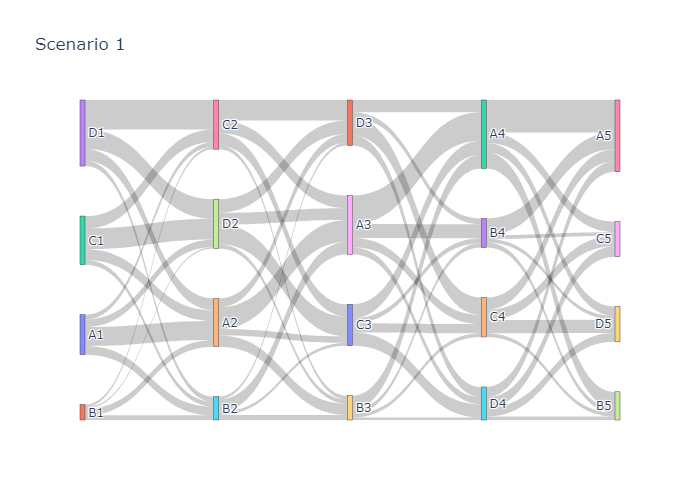
\includegraphics[width=\textwidth]{Figure/Figure26a.jpg}
    \caption{In scenario 1}
    \label{fig26a}
  \end{subfigure}
  \begin{subfigure}{0.5\textwidth}
    \centering
    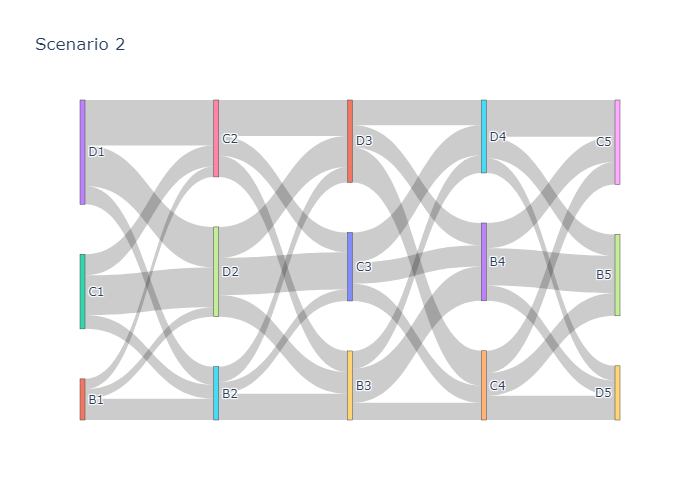
\includegraphics[width=\linewidth]{Figure/Figure26b.jpg}
    \caption{In scenario 2}
    \label{fig26b}
  \end{subfigure}
  \begin{subfigure}{0.5\textwidth}
    \centering
    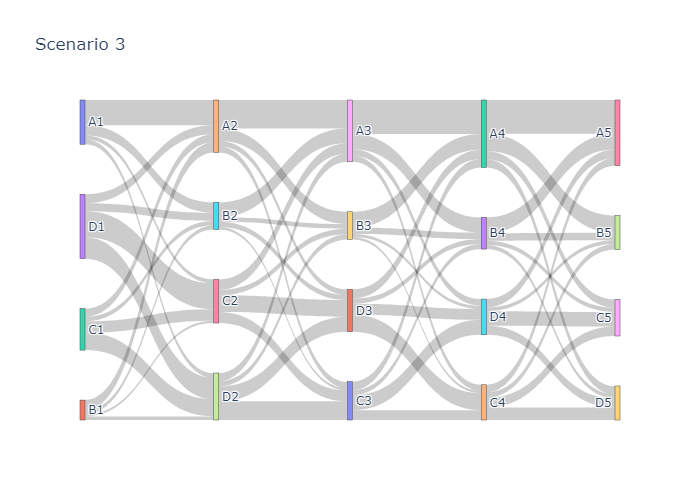
\includegraphics[width=\linewidth]{Figure/Figure26c.jpg}
    \caption{In scenario 3}
    \label{fig26c}
  \end{subfigure}
  \begin{subfigure}{0.5\textwidth}
    \centering
    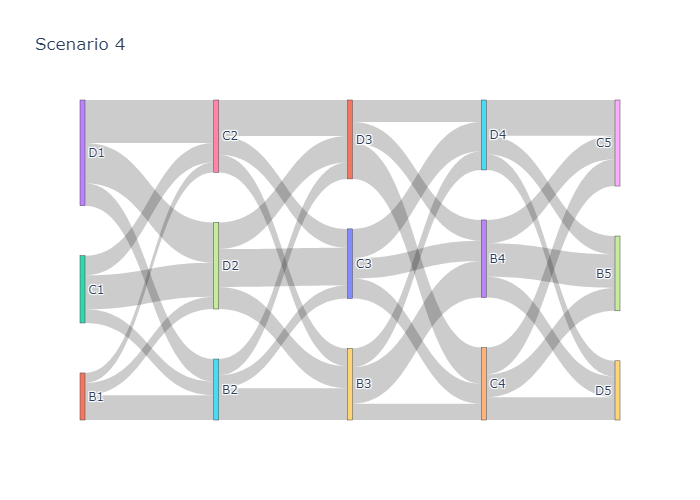
\includegraphics[width=\linewidth]{Figure/Figure26d.jpg}
    \caption{In scenario 4}
    \label{fig26d}
  \end{subfigure}
  \caption{Sankey diagram of foreign visitors }
  \label{fig26}
\end{figure*}

\begin{figure*}[h]
  \begin{subfigure}{0.5\textwidth}
    \centering
    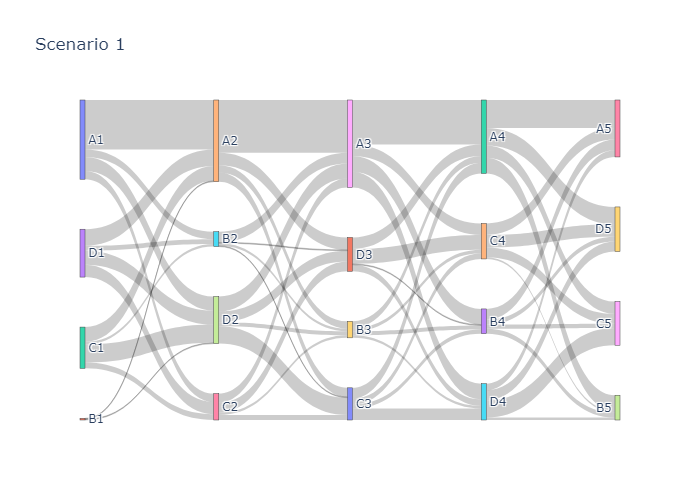
\includegraphics[width=\textwidth]{Figure/Figure27a.jpg}
    \caption{In scenario 1}
    \label{fig27a}
  \end{subfigure}
  \begin{subfigure}{0.5\textwidth}
    \centering
    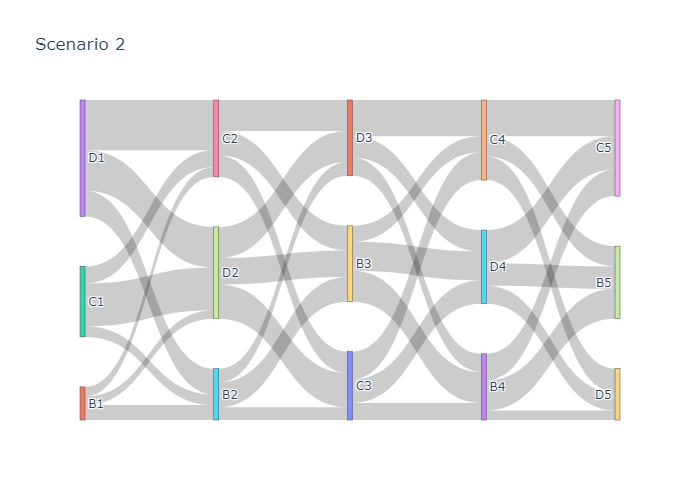
\includegraphics[width=\linewidth]{Figure/Figure27b.jpg}
    \caption{In scenario 2}
    \label{fig27b}
  \end{subfigure}
  \begin{subfigure}{0.5\textwidth}
    \centering
    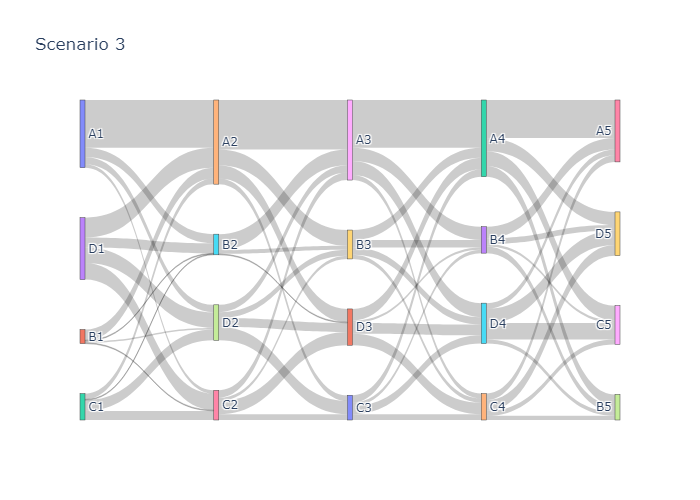
\includegraphics[width=\linewidth]{Figure/Figure27c.jpg}
    \caption{In scenario 3}
    \label{fig27c}
  \end{subfigure}
  \begin{subfigure}{0.5\textwidth}
    \centering
    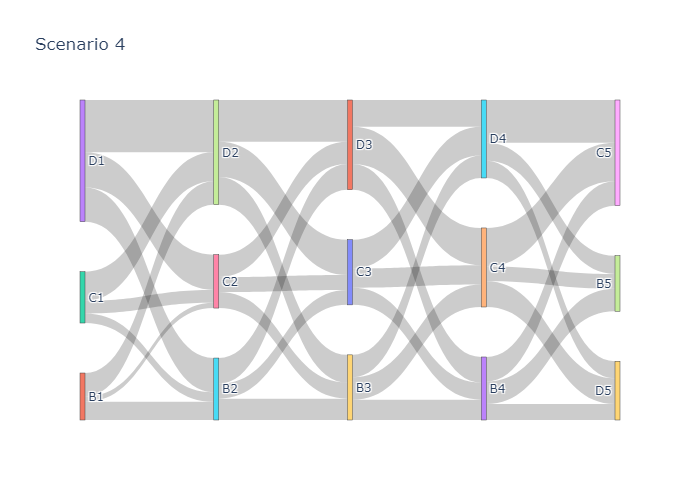
\includegraphics[width=\linewidth]{Figure/Figure27d.jpg}
    \caption{In scenario 4}
    \label{fig27d}
  \end{subfigure}
  \caption{Sankey diagram of Japanese }
  \label{fig27}
\end{figure*}

\begin{figure*}[h]
  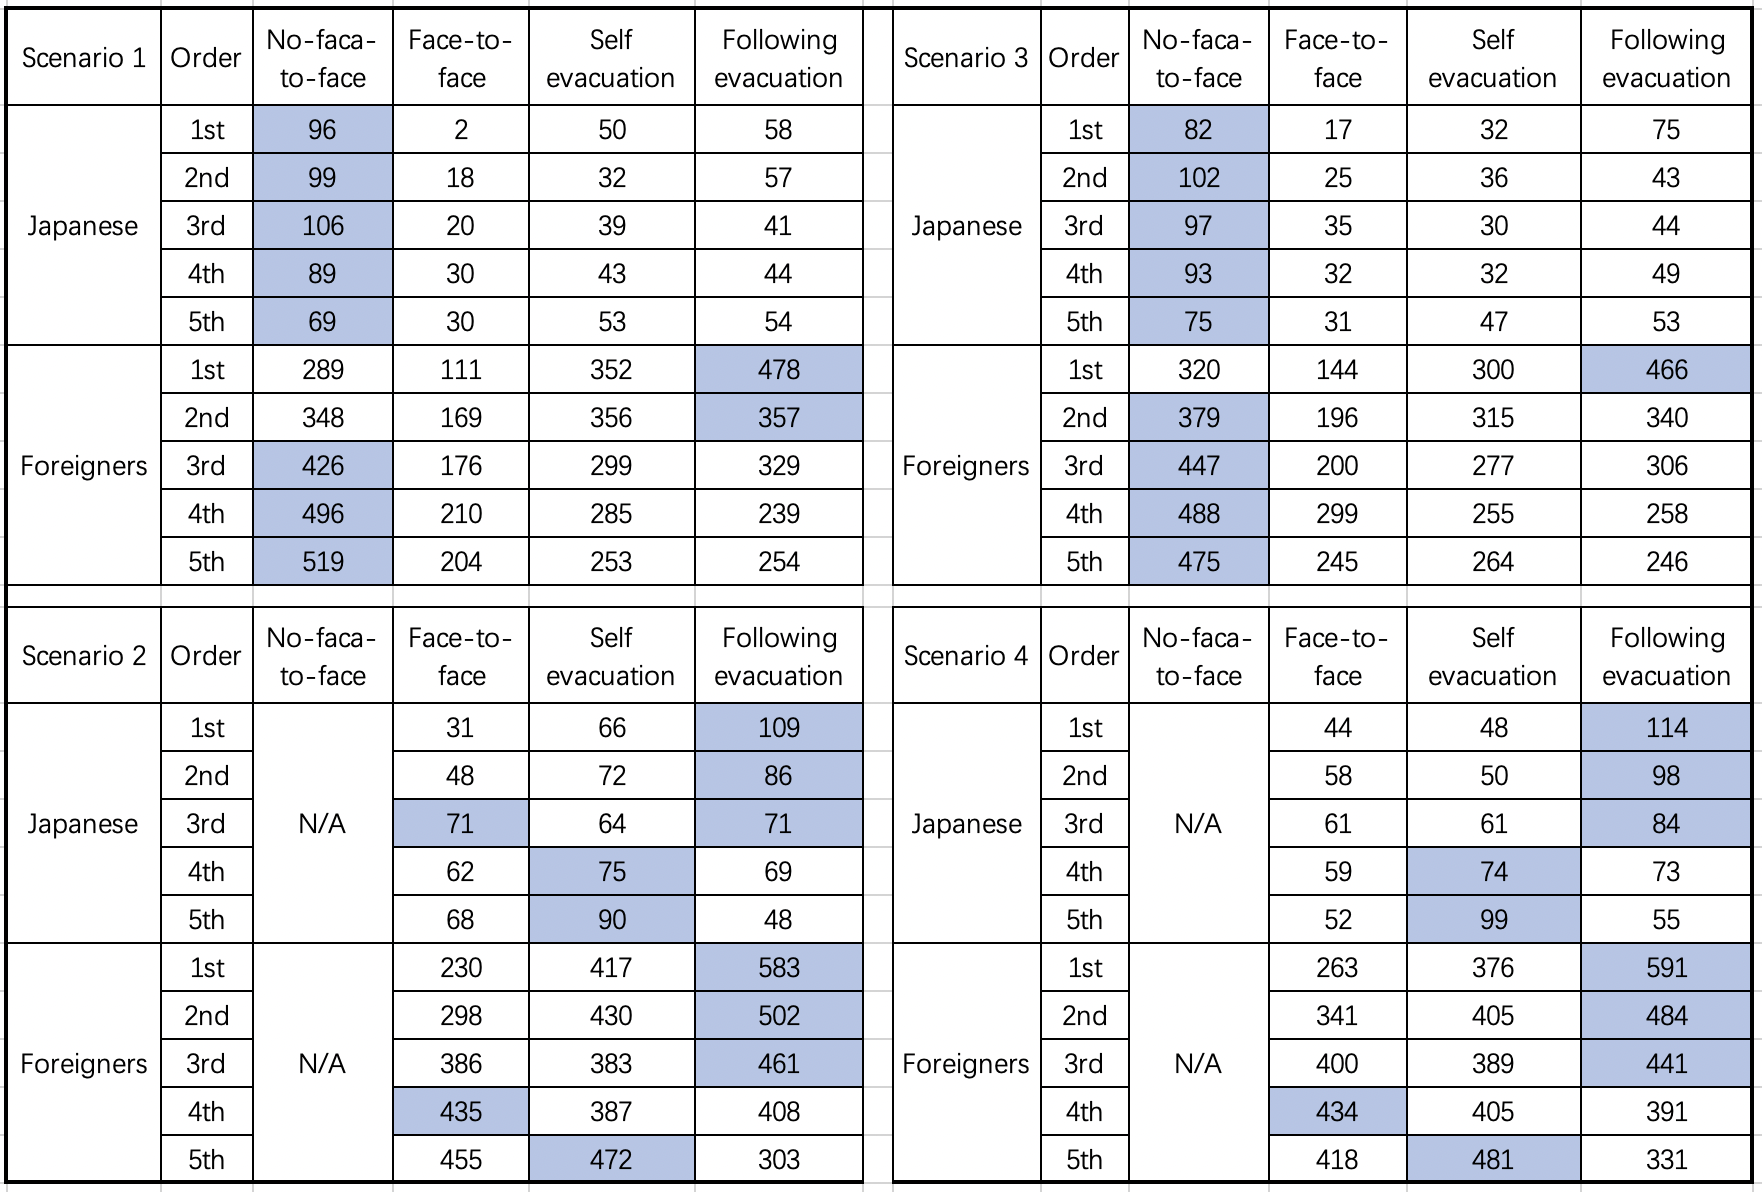
\includegraphics[width=\linewidth]{Figure/Figure28.jpg}
  \centering
  \caption{Summary of Sankey diagram data}
  \label{fig28}
\end{figure*}
%\fi








%% Some LaTeX commands I define for my own nomenclature.
% If you have to, it's better to change nomenclature once here than in a 
% million places throughout your thesis!



%======================================================================
\chapter{Objective 3: To explore categories of information seeking and evacuation behaviors.}
\label{c6}

\section{Methodology}

For research objective 3, this study wanted to explore respondents' information-seeking behaviors and evacuation behaviors through their selections of behaviors. In order to understand which of the behaviors are preferred and which are selected more frequently, we chose to measure both the selected rate and the selected score. The calculation of the selected rate and the selected score will both do three times, for 300 Japanese samples, 1500 foreign visitors samples, and 1800 of all respondents' samples.

\subsection{Selected Rate}
Because the selected rate wants to explore which behaviors are used more, this part does not take the order factor into account. No matter the behavior is selected in which order, it will count as 1 point. The selected rate is equal to the Sum selected point divided by the sample number, shown in Figure~\ref{fig10}.

%%%%%%%%%%%%%%%%%%%%%%%%%%%%
%\iffalse
\begin{figure*}[h]
  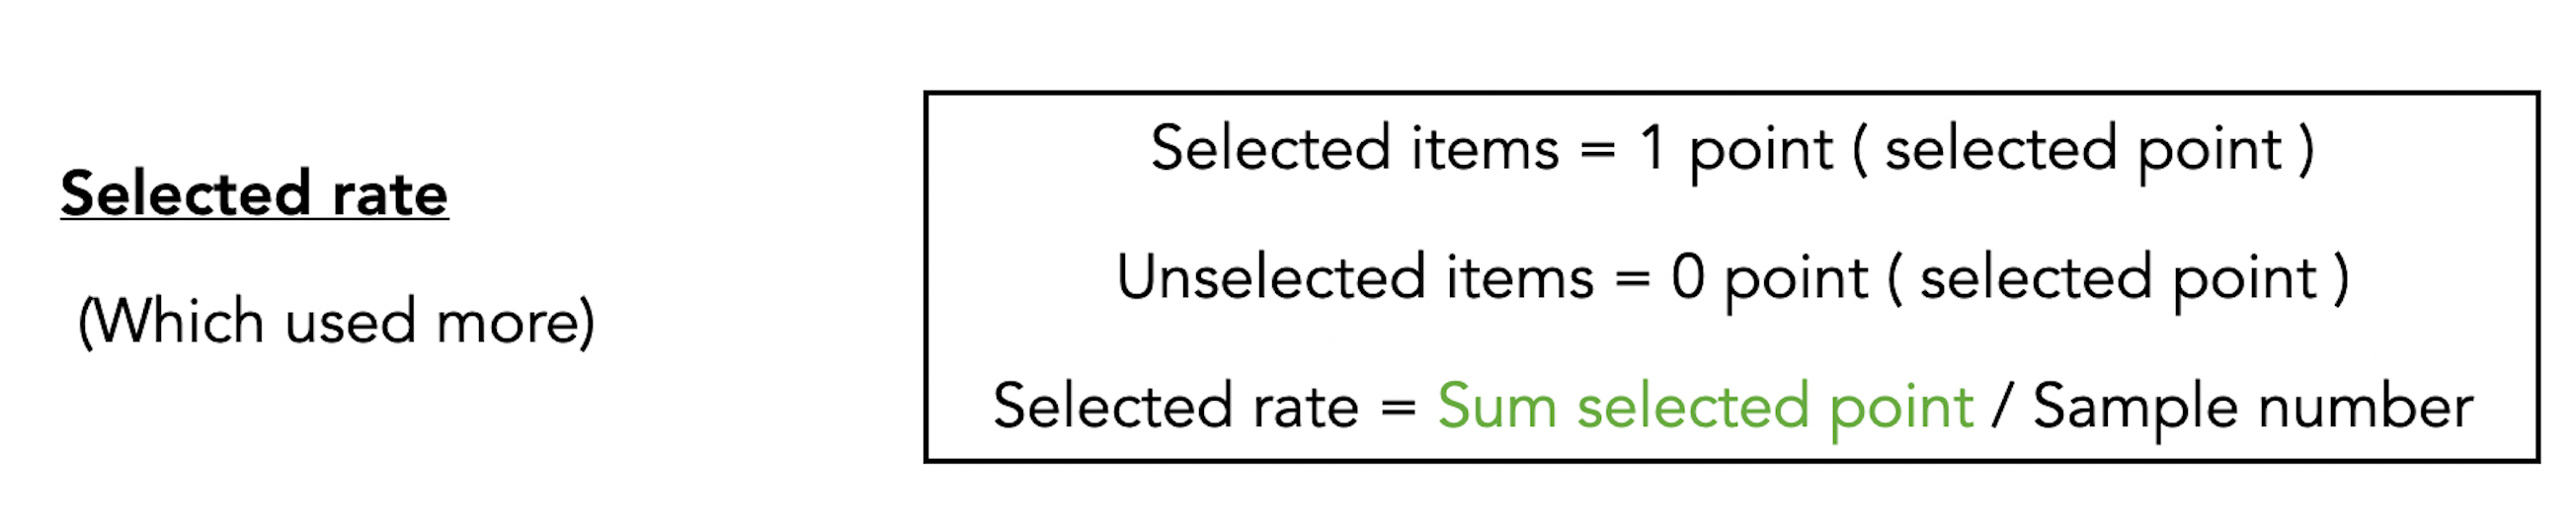
\includegraphics[width=\linewidth]{Figure/Figure10.png}
  \centering
  \caption{Selected rate }
  \label{fig10}
\end{figure*}
%\fi

\subsection{Selected Score}

Since the Selected score wants to explore which behaviors are used first, this part needs to take the order factor into account. The higher the preference is, the higher the score will be. So the first selected action is scored as 5, the second is scored as 4, the third is scored as 3, the fourth is scored as 2, and the last selected action is scored as 1. The Selected score is equal to the total score divided by the Sum selected point, shown in Figure~\ref{fig11}.

%%%%%%%%%%%%%%%%%%%%%%%%%%%
%\iffalse
\begin{figure*}[h]
  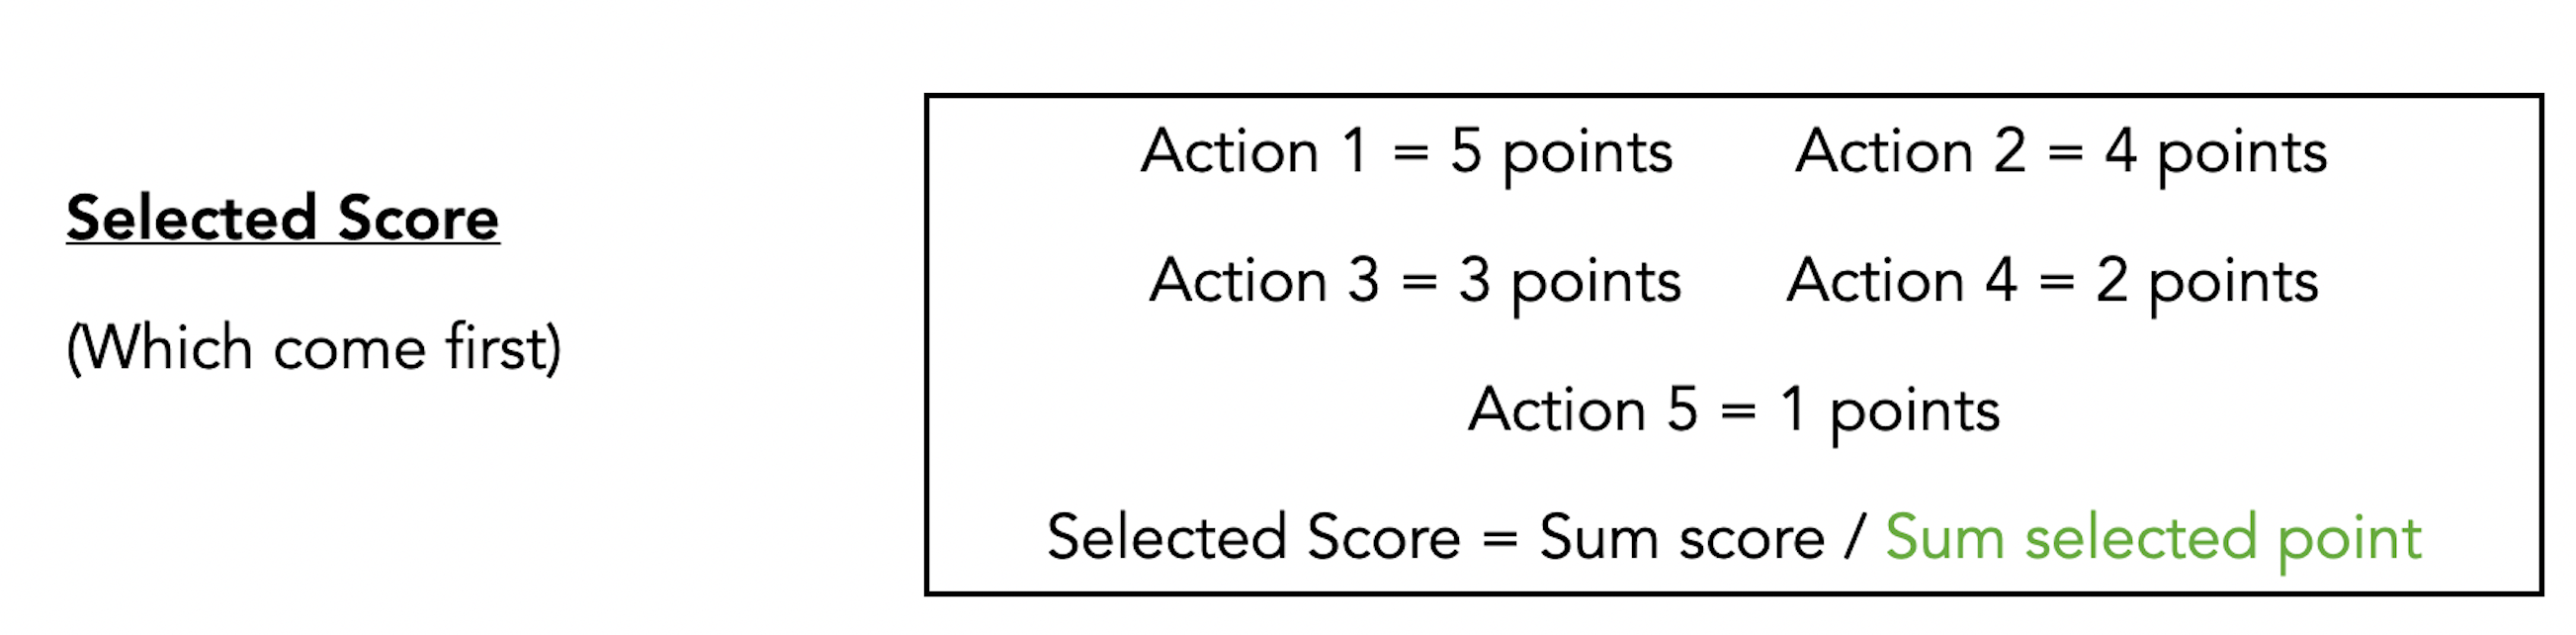
\includegraphics[width=\linewidth]{Figure/Figure11.png}
  \centering
  \caption{Selected score}
  \label{fig11}
\end{figure*}
%\fi

\subsection{Sankey Diagram of behavior categories}

In the analysis of the selected score and selected rate of study objective 3, we will find that all the results will be relatively scattered. This is because, in this study, the number of available selections is relatively large, which makes the results more scattered. However, from the results, we can see that there could be similarities in the behavior categories of people. Here the word 'pattern' means behavior categories, not specific behavior. For example, the behavior of  'collecting information' is the same, the difference is how to collect information, from official websites, from disaster prevention software, from disaster prevention websites, from SNS, etc. So how to divide detailed behaviors into categories? From the available selection, we can find that the behavior is mainly divided into two kinds, which are information-seeking behavior and evacuation behavior. First, regarding information-seeking behavior, we can find that there are two main categories, one is 'No-face-to-face information seeking' and the other is 'Face-to-face information seeking'. And for the evacuation behavior, we can also find two main categories, one is ' Self-evacuation behaviors ' and the other is ' Following evacuation guidance behavior '. Then, we divided all the selections into the categories they belong to, which can be found in Figure~\ref{fig12}.

%%%%%%%%%%%%%%%%%%%%%%%%%%%
%\iffalse
\begin{figure*}[h]
  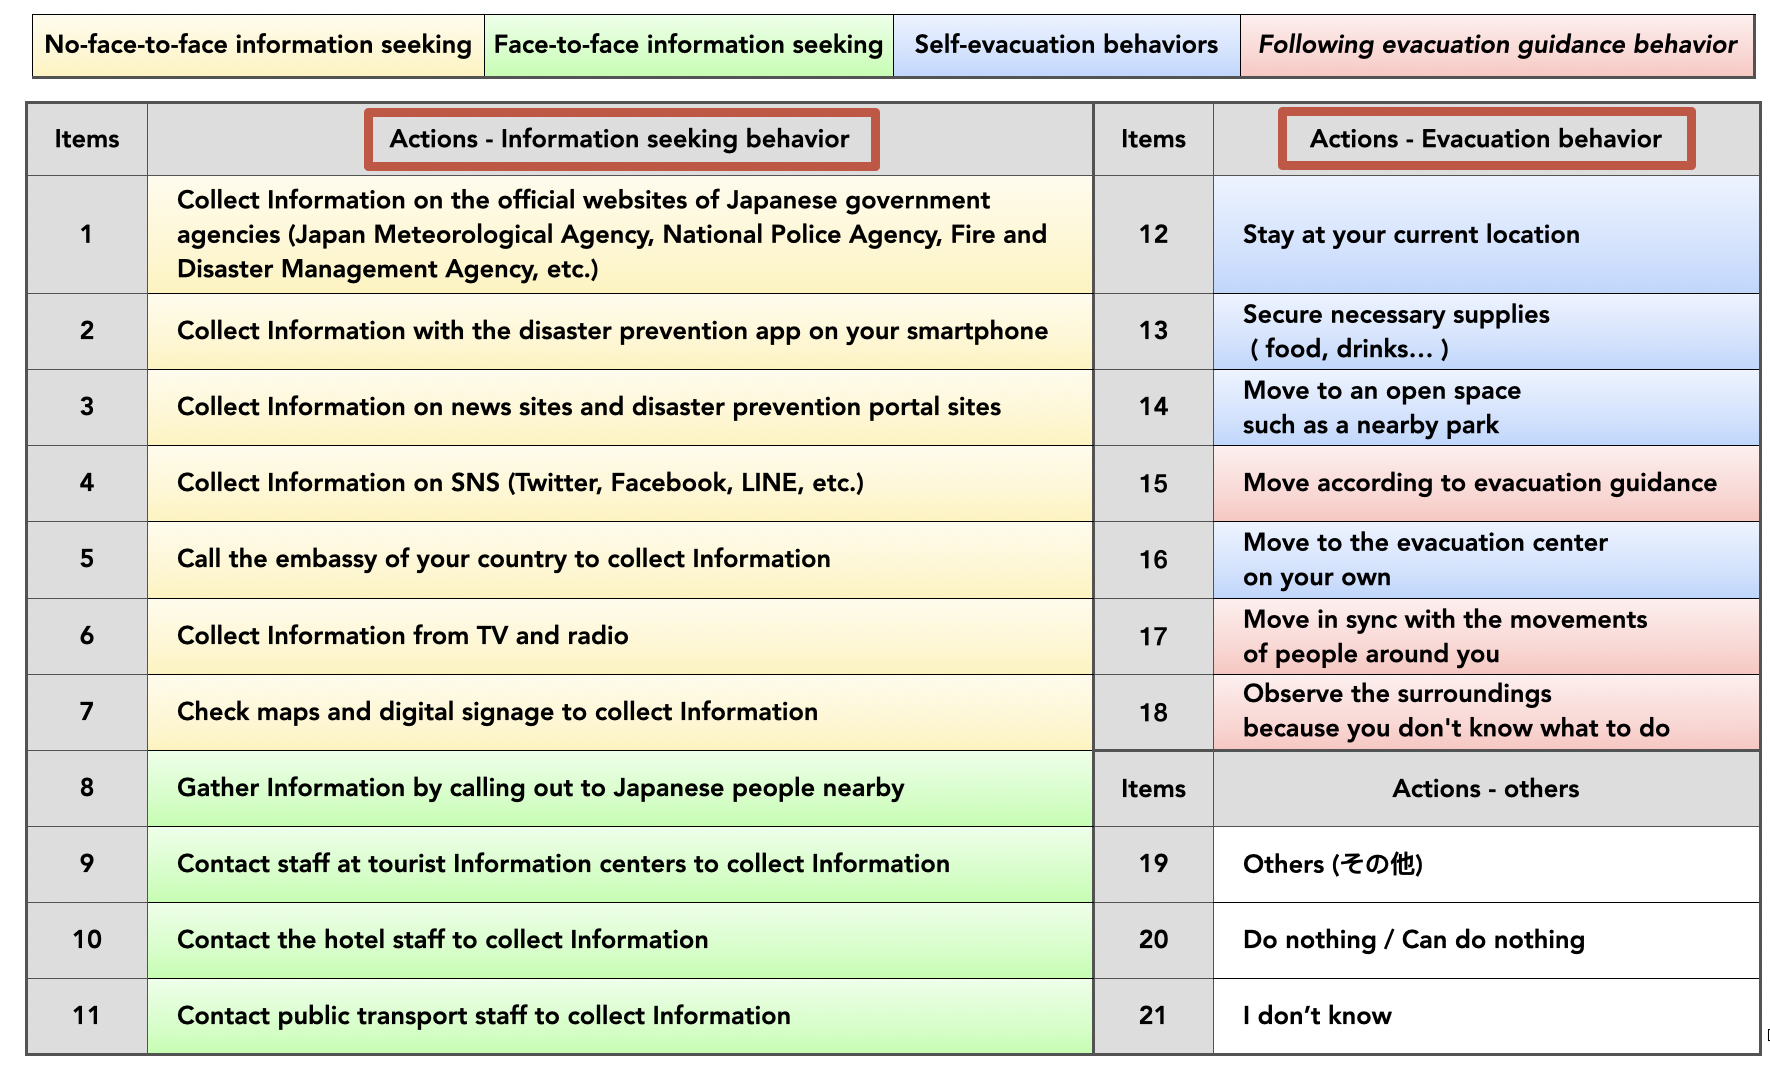
\includegraphics[width=\linewidth]{Figure/Figure12.png}
  \centering
  \caption{behavior categories}
  \label{fig12}
\end{figure*}
%\fi

After attributing all the actions to the 4 categories, we went through the flow of the respondents' actions with the help of the Sankey diagram. The Sankey diagram is a flow chart that shows the flow from each set of values to another set of values. The thickness of the lines expresses the number of values present in the group. In the Sankey diagram, the number indicates the No. of action, so 1-5 means the first action to the fifth action. Capital letters indicate behavior categories.' No-face-to-face information seeking' is A; 'Face-to-face information seeking' is B; 'Self-evacuation behaviors' is C; 'Following evacuation guidance behavior' is D. Thus, the behavior from the first to the fifth cohort can be clearly represented in the results of the Sankey diagram. As an example, A1 indicates that the 1st response action during the disaster is behavior pattern A, which is 'No-face-to-face information seeking'.






\section{Result}


\subsection{Selected Score and Selected Rate}
The result of the Selected score and the Selected rate is shown in \crefrange{table17}{table20}. From the result, we can find that there are some differences between foreign visitors and Japanese in scenarios 1 and 3, which could show that when the internet and telephone are available, people tend to have various behaviors. By checking the Selected Rate, we can find that evacuation behaviors are more used than information-seeking behaviors. And among the evacuation behaviors, 'Moving according to evacuation guidance' could be used most. This indicates that, regardless of the order factor, 'Moving according to evacuation guidance' is the most favored option. In addition, people are more likely to heed evacuation instructions if they are in the area of such recommendations.  By checking the Selected Score, we can find that evacuation behaviors always happen before information-seeking behaviors. And among the evacuation behaviors, 'Observe the surroundings' could have happened first. This is compounded by the fact that many people's first instinct in the event of a disaster is to observe others. Not only might they receive some evacuation suggestions, but keeping the same pace as others will make people feel more at ease psychologically. 

Some lower used information-seeking behaviors during a disaster are 'Gather Information by calling out to Japanese people nearby', 'Contact staff at tourist Information centers to collect Information', 'Contact public transport staff to collect Information'. As a result, in the case of Internet\&Phone available, people do not choose to acquire information through methods that require verbal conversation, and instead prefer to obtain it on their own. On the other hand, because people can only obtain information through the verbal conversation when the Internet and phone are unavailable, their method of obtaining information depends on the scenario they are in. When people are in a tourist area, they usually ask Japanese people around them for information, and not many people choose the other three options of contacting staff at different spots. However, when people are moving by transportation, people still ask Japanese people around them for information, while contacting staff from public transportation is also a popular option. The lowest used evacuation behavior during a disaster is 'Stay at your current location. This is understandable after all, few people will just stay put and do nothing in the face of a disaster. It is important to note here that this result does not mean that everyone will necessarily do something to leave the place where it happened, but that people's priority evacuation behavior is less likely to be to stay where they are. People will, in most situations, choose to remain where they are after gathering information and following evacuation instructions. This section does not cover such circumstances.

%%%%%%%%%%%%%%%%%%%%%%%%%%
%\iffalse
\begin{table}[h]
  \caption[Result of Selected score and Selected rate in Scenario 1]{Result of Selected score and Selected rate in Scenario 1(No.: number of  selection, FV: Foreign Vistors, J: Japanese)}
  \label{table17}
  \centering 
  \begin{tabular}{cl|ccc|ccc}
                &   & \multicolumn{3}{c}{Selected Rate (\%)} & \multicolumn{3}{c}{Selected Score} \\
      No.     & \multicolumn{1}{c|}{Description} & All & FV & J & All & FV & J \\
 \hline
  1             & \begin{tabular}{l}Collect Information on the official websites\\of Japanese government agencies\end{tabular} & 31.6 &30.2 & 38.7 & 2.9 & 2.9 & 3.0 \\
  2             & \begin{tabular}{l}Collect Information with the disaster\\prevention app on your smartphone\end{tabular} & 27.9 & 25.4 & 40.7 & 2.9 & 2.8 & 3.2 \\
  3             & \begin{tabular}{l}Collect Information on news sites and\\disaster prevention portal sites\end{tabular} & 26.8 & 23.4 & 43.7 & 2.8 & 2.7 & 3.2 \\
  4             & \begin{tabular}{l}Collect Information on SNS\\(Twitter, Facebook, LINE, etc.)\end{tabular} & 19.9 & 18.2 & 28.7 & 2.8 & 2.7 & 3.0 \\
  5             & \begin{tabular}{l}Call the embassy of your country\\to collect Information\end{tabular} & 25.2 & 30.3 & N/A & 2.7 & 2.7 & N/A \\
  6             & \begin{tabular}{l}Collect Information from TV and radio\end{tabular} & 24.9 & 20.9 & 44.7 & 3.0 & 2.8 & 3.4 \\
  7             & \begin{tabular}{l}Check maps and digital signage to\\collect Information\end{tabular} & 14.4 & 15.0 & 11.7 & 2.8 & 2.8 & 2.9 \\
  8             & \begin{tabular}{l}Gather Information by calling out to\\Japanese people nearby\end{tabular} & 18.7 & 19.0 & 17.3 & 2.7 & 2.8 & 2.3 \\
  9             & \begin{tabular}{l}Contact staff at tourist Information\\centers to collect Information\end{tabular} & 16.0 & 18.3 & 4.3 & 2.9 & 2.9 & 2.3 \\
 10            & \begin{tabular}{l}Contact the hotel staff to collect\\Information\end{tabular} & 15.8 & 17.0 & 10.0 & 2.8 & 2.8 & 2.8 \\
 11            & \begin{tabular}{l}Contact public transport staff to\\collect Information\end{tabular} & 13.9 & 13.7 & 14.7 & 2.5 & 2.6 & 2.4 \\
 12            & \begin{tabular}{l}Stay at your current location\end{tabular} & 16.6 & 17.5 & 12.0 & 3.4 & 3.4 & 3.5 \\
 13            & \begin{tabular}{l}Secure necessary supplies\\(food, drink, etc.)\end{tabular}  & 32.9 & 33.0 & 32.3 & 3.0 & 3.1 & 2.8 \\
 14            & \begin{tabular}{l}Move to an open space such as a\\nearby park\end{tabular} & 39.7 & 41.8 & 29.0 & 3.3 & 3.3 & 3.0 \\
 15            & \begin{tabular}{l}Move according to evacuation\\guidance\end{tabular} & 53.7 & 54.9 & 47.7 & 3.4 & 3.5 & 3.2 \\
 16            & \begin{tabular}{l}Move to the evacuation center on\\your own\end{tabular} & 26.8 & 27.1 & 25.0 & 3.1 & 3.1 & 3.0 \\
 17            & \begin{tabular}{l}Move in sync with the movements\\of people around you\end{tabular} & 28.3 & 29.2 & 24.0 & 2.8 & 2.9 & 2.6 \\
 18            & \begin{tabular}{l}Observe the surroundings because\\you don't know what to do\end{tabular} & 45.2 & 44.7 & 48.0 & 3.6 & 3.6 & 3.4 \\
\hline
  \end{tabular}
\end{table}


\begin{table}[h]
  \caption[Result of Selected score and Selected rate in Scenario 2]{Result of Selected score and Selected rate in Scenario 2(No.: number of  selection, FV: Foreign Vistors, J: Japanese)}
  \label{table18}
  \centering 
  \begin{tabular}{cl|ccc|ccc}
                &   & \multicolumn{3}{c}{Selected Rate (\%)} & \multicolumn{3}{c}{Selected Score} \\
      No.     & \multicolumn{1}{c|}{Description} & All & FV & J & All & FV & J \\
 \hline
  8             & \begin{tabular}{l}Gather Information by calling out to\\Japanese people nearby\end{tabular} & 41.1 & 40.5 & 44.0 & 2.8 & 2.8 & 2.9 \\
  9             & \begin{tabular}{l}Contact staff at tourist Information\\centers to collect Information\end{tabular} & 33.8 & 36.8 & 18.7 & 2.7 & 2.7 & 2.4 \\
 10            & \begin{tabular}{l}Contact the hotel staff to collect\\Information\end{tabular} & 33.0 & 34.3 & 26.7 & 2.9 & 2.8 & 3.0 \\
 11            & \begin{tabular}{l}Contact public transport staff to\\collect Information\end{tabular} & 29.8 & 29.3 & 32.7 & 2.7 & 2.6 & 2.8 \\
 12            & \begin{tabular}{l}Stay at your current location\end{tabular} & 23.9 & 24.7 & 20.0 & 3.0 & 3.0 & 3.0 \\
 13            & \begin{tabular}{l}Secure necessary supplies\\(food, drink, etc.)\end{tabular}  & 44.5 & 44.4 & 45.0 & 2.9 & 2.9 & 3.0 \\
 14            & \begin{tabular}{l}Move to an open space such as a\\nearby park\end{tabular} & 52.5 & 54.5 & 44.7 & 3.2 & 3.2 & 3.1 \\
 15            & \begin{tabular}{l}Move according to evacuation\\guidance\end{tabular} & 66.6 & 65.9 & 70.0 & 3.4 & 3.4 & 3.5 \\
 16            & \begin{tabular}{l}Move to the evacuation center on\\your own\end{tabular} & 39.3 & 37.9 & 46.3 & 2.9 & 2.9 & 2.7 \\
 17            & \begin{tabular}{l}Move in sync with the movements\\of people around you\end{tabular} & 46.5 & 47.3 & 42.7 & 2.9 & 3.0 & 2.8 \\
 18            & \begin{tabular}{l}Observe the surroundings because\\you don't know what to do\end{tabular} & 61.6 & 60.7 & 66.0 & 3.6 & 3.5 & 3.8 \\
\hline
  \end{tabular}
\end{table}



\begin{table}[h]
  \caption[Result of Selected score and Selected rate in Scenario 3]{Result of Selected score and Selected rate in Scenario 3(No.: number of  selection, FV: Foreign Vistors, J: Japanese)}
  \label{table19}
  \centering 
  \begin{tabular}{cl|ccc|ccc}
                &   & \multicolumn{3}{c}{Selected Rate (\%)} & \multicolumn{3}{c}{Selected Score} \\
      No.     & \multicolumn{1}{c|}{Description} & All & FV & J & All & FV & J \\
 \hline
  1             & \begin{tabular}{l}Collect Information on the official websites\\of Japanese government agencies\end{tabular} & 29.1 & 28.6 & 31.1 & 3.0 & 3.0 & 3.0 \\
  2             & \begin{tabular}{l}Collect Information with the disaster\\prevention app on your smartphone\end{tabular} & 29.4 & 27.1 & 41.0 & 3.0 & 2.9 & 3.2 \\
  3             & \begin{tabular}{l}Collect Information on news sites and\\disaster prevention portal sites\end{tabular} & 27.6 & 24.5 & 43.0 & 2.8 & 2.7 & 3.2 \\
  4             & \begin{tabular}{l}Collect Information on SNS\\(Twitter, Facebook, LINE, etc.)\end{tabular} & 24.6 & 22.7 & 34.3 & 2.8 & 2.7 & 3.0 \\
  5             & \begin{tabular}{l}Call the embassy of your country\\to collect Information\end{tabular} & 24.2 & 29.0 & N/A & 2.9 & 2.9 & N/A \\
  6             & \begin{tabular}{l}Collect Information from TV and radio\end{tabular} & 22.4 & 19.3 & 37.7 & 2.9 & 2.8 & 3.0 \\
  7             & \begin{tabular}{l}Check maps and digital signage to\\collect Information\end{tabular} & 15.7 & 16.2 & 13.3 & 2.9 & 2.9 & 2.9 \\
  8             & \begin{tabular}{l}Gather Information by calling out to\\Japanese people nearby\end{tabular} & 20.7 & 21.1 & 18.3 & 2.7 & 2.7 & 2.7 \\
  9             & \begin{tabular}{l}Contact staff at tourist Information\\centers to collect Information\end{tabular} & 16.8 & 18.8 & 7.0 & 2.7 & 2.7 & 2.7 \\
 10            & \begin{tabular}{l}Contact the hotel staff to collect\\Information\end{tabular} & 15.4 & 17.1 & 7.0 & 2.8 & 2.8 & 2.9 \\
 11            & \begin{tabular}{l}Contact public transport staff to\\collect Information\end{tabular} & 23.9 & 22.6 & 30.7 & 3.0 & 3.0 & 3.1 \\
 12            & \begin{tabular}{l}Stay at your current location\end{tabular} & 13.7 & 14.3 & 10.3 & 3.6 & 3.7 & 2.9 \\
 13            & \begin{tabular}{l}Secure necessary supplies\\(food, drink, etc.)\end{tabular}  & 27.8 & 28.3 & 25.3 & 3.0 & 3.0 & 2.9 \\
 14            & \begin{tabular}{l}Move to an open space such as a\\nearby park\end{tabular} & 34.6 & 37.6 & 19.3 & 3.2 & 3.2 & 2.9 \\
 15            & \begin{tabular}{l}Move according to evacuation\\guidance\end{tabular} & 50.7 & 50.9 & 50.0 & 3.4 & 3.4 & 3.2 \\
 16            & \begin{tabular}{l}Move to the evacuation center on\\your own\end{tabular} & 26.6 & 27.9 & 20.3 & 2.9 & 2.9 & 2.8 \\
 17            & \begin{tabular}{l}Move in sync with the movements\\of people around you\end{tabular} & 32.4 & 33.6 & 26.7 & 2.9 & 2.9 & 2.8 \\
 18            & \begin{tabular}{l}Observe the surroundings because\\you don't know what to do\end{tabular} & 41.1 & 40.8 & 42.7 & 3.7 & 3.7 & 3.5 \\
\hline
  \end{tabular}
\end{table}


\begin{table}[h]
  \caption[Result of Selected score and Selected rate in Scenario 4]{Result of Selected score and Selected rate in Scenario 4(No.: number of  selection, FV: Foreign Vistors, J: Japanese)}
  \label{table20}
  \centering 
  \begin{tabular}{cl|ccc|ccc}
                &   & \multicolumn{3}{c}{Selected Rate (\%)} & \multicolumn{3}{c}{Selected Score} \\
      No.     & \multicolumn{1}{c|}{Description} & All & FV & J & All & FV & J \\
 \hline
  8             & \begin{tabular}{l}Gather Information by calling out to\\Japanese people nearby\end{tabular} & 42.3 & 43.4 & 37.0 & 2.8 & 2.8 & 2.8 \\
  9             & \begin{tabular}{l}Contact staff at tourist Information\\centers to collect Information\end{tabular} & 29.2 & 32.1 & 14.7 & 2.7 & 2.7 & 2.7 \\
 10            & \begin{tabular}{l}Contact the hotel staff to collect\\Information\end{tabular} & 27.2 & 29.5 & 15.7 & 2.9 & 2.9 & 2.8 \\
 11            & \begin{tabular}{l}Contact public transport staff to\\collect Information\end{tabular} & 40.9 & 39.4 & 48.3 & 3.1 & 3.0 & 3.4 \\
 12            & \begin{tabular}{l}Stay at your current location\end{tabular} & 24.3 & 24.8 & 21.7 & 3.1 & 3.2 & 3.0 \\
 13            & \begin{tabular}{l}Secure necessary supplies\\(food, drink, etc.)\end{tabular}  & 39.1 & 39.2 & 38.3 & 2.8 & 2.9 & 2.8 \\
 14            & \begin{tabular}{l}Move to an open space such as a\\nearby park\end{tabular} & 49.8 & 52.2 & 37.7 & 3.0 & 3.0 & 2.6 \\
 15            & \begin{tabular}{l}Move according to evacuation\\guidance\end{tabular} & 67.7 & 66.2 & 75.0 & 3.5 & 3.4 & 3.6 \\
 16            & \begin{tabular}{l}Move to the evacuation center on\\your own\end{tabular} & 41.1 & 40.9 & 42.0 & 2.8 & 2.8 & 2.5 \\
 17            & \begin{tabular}{l}Move in sync with the movements\\of people around you\end{tabular} & 50.6 & 50.9 & 49.0 & 2.9 & 3.0 & 2.8 \\
 18            & \begin{tabular}{l}Observe the surroundings because\\you don't know what to do\end{tabular} & 59.2 & 57.5 & 67.7 & 3.5 & 3.5 & 3.6 \\
\hline
  \end{tabular}
\end{table}
%\fi
\cleardoublepage
\subsection{Sankey Diagram of behavior categories}

Summary of the Sankey Diagram data is shown in Figure~\ref{fig28}, blue denoting the action with the highest rate. 

\begin{figure*}[h]
  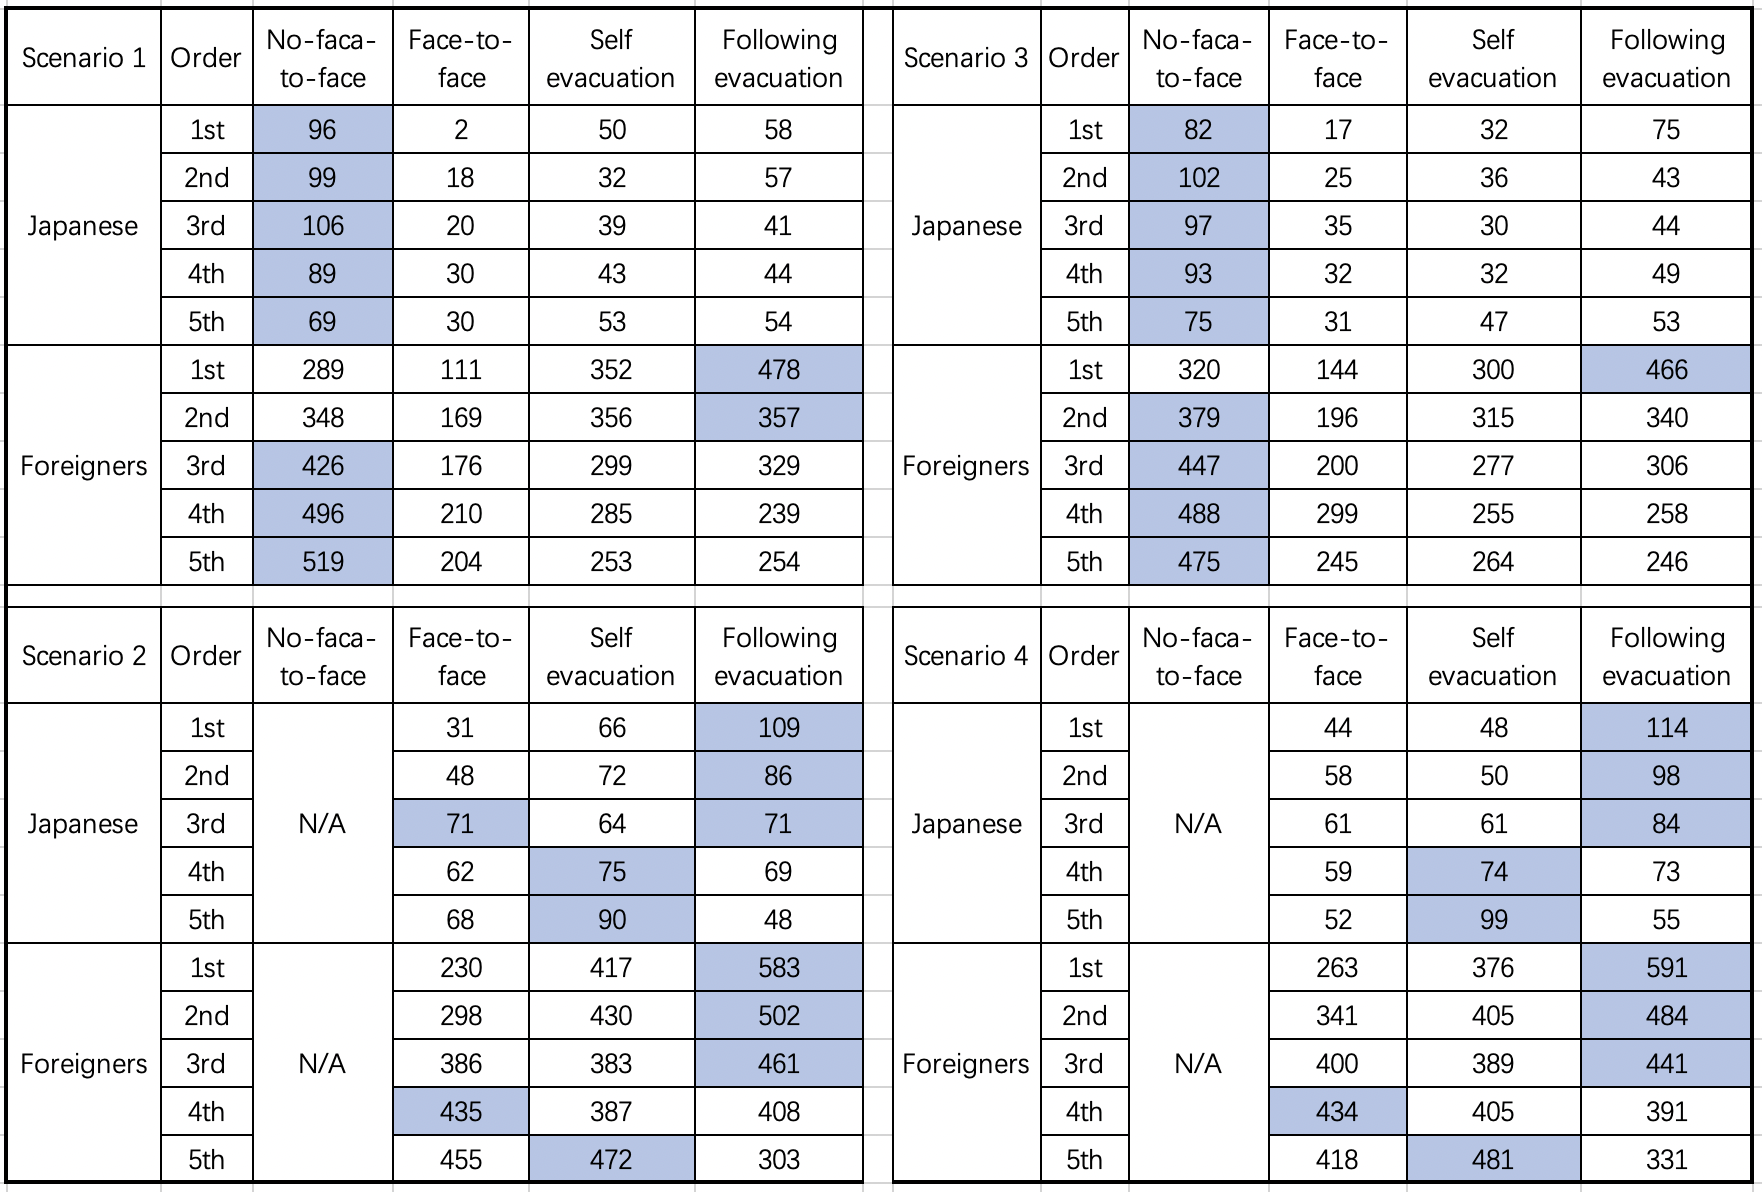
\includegraphics[width=\linewidth]{Figure/Figure28.jpg}
  \centering
  \caption{Summary of Sankey diagram data}
  \label{fig28}
\end{figure*}

We can learn from the data that No-face-to-face information seeking is more common than face-to-face information seeking. In the top three actions, following evacuation guidance behaviors is more common than self-evacuation behaviors. 

The Sankey Diagram for foreign visitors and Japanese in scenarios 1 to 4 is depicted in \crefrange{fig26a}{fig26d}. By the Sankey diagram, we can clearly find that there are many differences between Japanese and foreign visitors. In scenario 1(Figure~\ref{fig26a}),  the internet and telephone are available, and respondents are staying in a tourist attraction. The result shows Japanese always prefer to seek information, the rate of selecting  No-face-to-face information-seeking behaviors from the first order to the fifth-order is always higher than other behavior categories. In Particular, the top three behaviors are almost 50\%.  However, for foreign visitors, the first and the second behavior show differences from the Japanese. Foreign visitors prefer to start by following evacuation guidance behaviors, and then start to seek information.  In scenario 2(Figure~\ref{fig26c}), respondents are still staying in a tourist attraction, but the internet and telephone are unavailable this time. The result shows that the behaviors of Japanese and foreign visitors show some similarities. They both start from following evacuation guidance behaviors, and then face-to-face information seeking, finally self-evacuation behaviors.  In scenario 2(Figure~\ref{fig26b}) and scenario 4(Figure~\ref{fig26d}) respondents are moving by public transportation, the results show similar with scenario 1 and scenario 3. This can indicate that respondents' behaviors are not much affected by their situation, but affected by whether the internet and telephone are available or not. 

%%%%%%%%%%%%%%%%%%%%%%%%%%
%\iffalse
\begin{figure*}[h]
  \begin{subfigure}{0.5\textwidth}
    \centering
    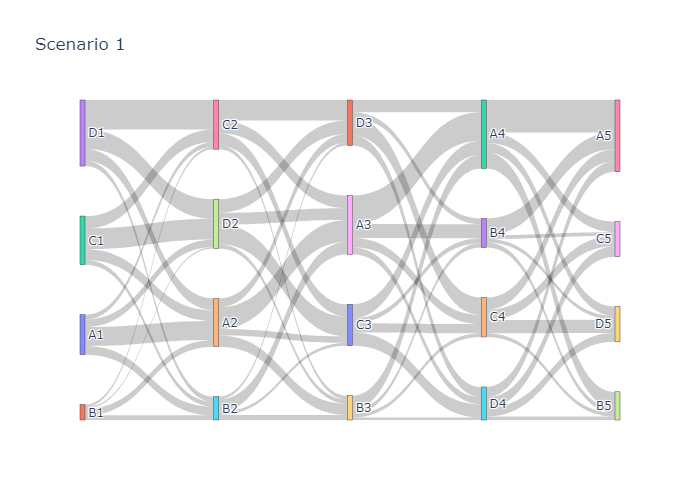
\includegraphics[width=\textwidth]{Figure/Figure26a.jpg}
    \caption{Japanese}
  \end{subfigure}
  \begin{subfigure}{0.5\textwidth}
    \centering
    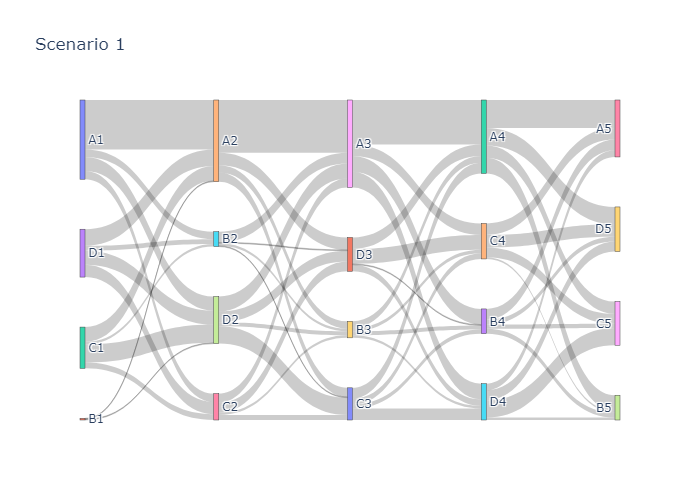
\includegraphics[width=\linewidth]{Figure/Figure27a.jpg}
    \caption{Foreign visitors}
  \end{subfigure}
  \caption{Sankey diagram of in senario 1 }
  \label{fig26a}
\end{figure*}

\begin{figure*}[h]
  \begin{subfigure}{0.5\textwidth}
    \centering
    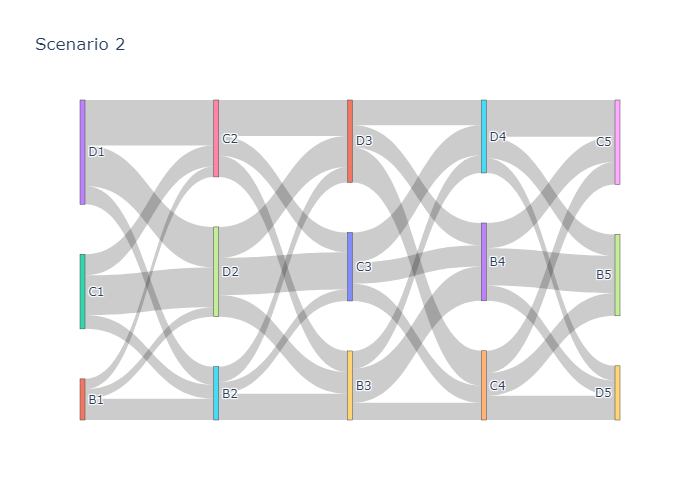
\includegraphics[width=\textwidth]{Figure/Figure26b.jpg}
    \caption{Japanese}
  \end{subfigure}
  \begin{subfigure}{0.5\textwidth}
    \centering
    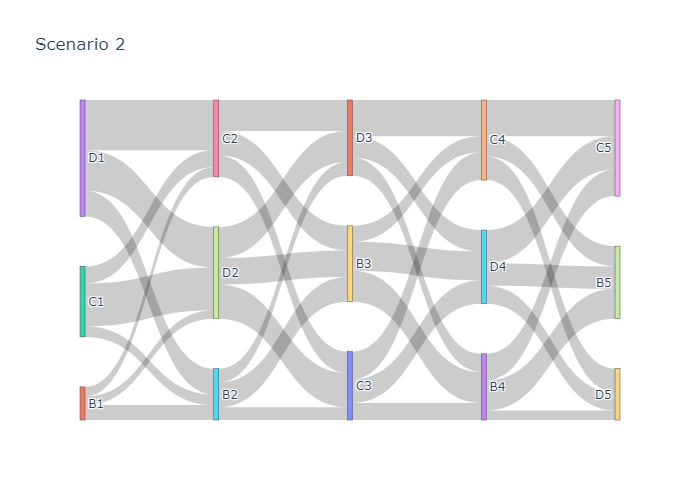
\includegraphics[width=\linewidth]{Figure/Figure27b.jpg}
    \caption{Foreign visitors}
  \end{subfigure}
  \caption{Sankey diagram of in senario 2 }
  \label{fig26b}
\end{figure*}

\begin{figure*}[h]
  \begin{subfigure}{0.5\textwidth}
    \centering
    \includegraphics[width=\textwidth]{Figure/Figure26c.jpg}
    \caption{Japanese}
  \end{subfigure}
  \begin{subfigure}{0.5\textwidth}
    \centering
    \includegraphics[width=\linewidth]{Figure/Figure27c.jpg}
    \caption{Foreign visitors}
  \end{subfigure}
  \caption{Sankey diagram of in senario 3 }
  \label{fig26c}
\end{figure*}

\begin{figure*}[h]
  \begin{subfigure}{0.5\textwidth}
    \centering
    \includegraphics[width=\textwidth]{Figure/Figure26d.jpg}
    \caption{Japanese}
  \end{subfigure}
  \begin{subfigure}{0.5\textwidth}
    \centering
    \includegraphics[width=\linewidth]{Figure/Figure27d.jpg}
    \caption{Foreign visitors}
  \end{subfigure}
  \caption{Sankey diagram of in senario 4 }
  \label{fig26d}
\end{figure*}


We can more clearly see the differences between foreign visitors and Japanese when we attribute specific actions to behavior patterns. The most common actions among Japanese in scenarios 1 and 3 are all No-face-to-face information seeking, but the most common behaviors among foreign tourists are following evacuation guidance behaviors, followed by No-face-to-face information seeking. In summary, when the internet and telephone are available, Japanese prefer to take No-face-to-face information-seeking behaviors, while foreign visitors prefer to follow evacuation guidance behavior first, then trend to take No-face-to-face information-seeking behaviors. When the internet and phone are unavailable, both Japanese and foreign visitors show similar behavior. Both Japanese and foreigners prefer to follow evacuation guidance behaviors first. However, there are some differences in the behaviors that followed. Self-evacuation behaviors are preferred by the Japanese, while foreigners prefer face-to-face information-seeking behaviors before self-evacuation behaviors.


We also used the Sankey diagram to analyze the flow of respondents' response actions in each country. The results are shown in \crefrange{fig32}{fig35}. But from the graph we can actually hardly see the difference, basically, the action selection is similar in terms of ratio for each cis. This proves that there is little variability among foreigners and people's actions are not influenced by differences in home country nationality.



\begin{figure*}[h]
  \begin{subfigure}{0.5\textwidth}
    \centering
    \includegraphics[width=\textwidth]{Figure/figure32a.png}
    \caption{Indonesia}
  \end{subfigure}
  \begin{subfigure}{0.5\textwidth}
    \centering
    \includegraphics[width=\linewidth]{Figure/figure33a.png}
    \caption{South Korea}
  \end{subfigure}
  \begin{subfigure}{0.5\textwidth}
    \centering
    \includegraphics[width=\linewidth]{Figure/figure34a.png}
    \caption{Thailand}
  \end{subfigure}
  \begin{subfigure}{0.5\textwidth}
    \centering
    \includegraphics[width=\linewidth]{Figure/figure35a.png}
    \caption{the UK}
  \end{subfigure}
  \begin{subfigure}{0.5\textwidth}
    \centering
    \includegraphics[width=\linewidth]{Figure/figure36a.png}
    \caption{China}
  \end{subfigure}
  \caption{ Sankey diagram of foreign vistors in senario 1 }
  \label{fig32}
\end{figure*}

\begin{figure*}[h]
  \begin{subfigure}{0.5\textwidth}
    \centering
    \includegraphics[width=\textwidth]{Figure/figure32b.png}
    \caption{Indonesia}
  \end{subfigure}
  \begin{subfigure}{0.5\textwidth}
    \centering
    \includegraphics[width=\linewidth]{Figure/figure33b.png}
    \caption{South Korea}
  \end{subfigure}
  \begin{subfigure}{0.5\textwidth}
    \centering
    \includegraphics[width=\linewidth]{Figure/figure34b.png}
    \caption{Thailand}
  \end{subfigure}
  \begin{subfigure}{0.5\textwidth}
    \centering
    \includegraphics[width=\linewidth]{Figure/figure35b.png}
    \caption{the UK}
  \end{subfigure}
  \begin{subfigure}{0.5\textwidth}
    \centering
    \includegraphics[width=\linewidth]{Figure/figure36b.png}
    \caption{China}
  \end{subfigure}
  \caption{ Sankey diagram of foreign vistors in senario 2 }
  \label{fig33}
\end{figure*}

\begin{figure*}[h]
  \begin{subfigure}{0.5\textwidth}
    \centering
    \includegraphics[width=\textwidth]{Figure/figure32c.png}
    \caption{Indonesia}
  \end{subfigure}
  \begin{subfigure}{0.5\textwidth}
    \centering
    \includegraphics[width=\linewidth]{Figure/figure33c.png}
    \caption{South Korea}
  \end{subfigure}
  \begin{subfigure}{0.5\textwidth}
    \centering
    \includegraphics[width=\linewidth]{Figure/figure34c.png}
    \caption{Thailand}
  \end{subfigure}
  \begin{subfigure}{0.5\textwidth}
    \centering
    \includegraphics[width=\linewidth]{Figure/figure35c.png}
    \caption{the UK}
  \end{subfigure}
  \begin{subfigure}{0.5\textwidth}
    \centering
    \includegraphics[width=\linewidth]{Figure/figure36c.png}
    \caption{China}
  \end{subfigure}
  \caption{ Sankey diagram of foreign vistors in senario 3 }
  \label{fig34}
\end{figure*}

\begin{figure*}[h]
  \begin{subfigure}{0.5\textwidth}
    \centering
    \includegraphics[width=\textwidth]{Figure/figure32d.png}
    \caption{Indonesia}
  \end{subfigure}
  \begin{subfigure}{0.5\textwidth}
    \centering
    \includegraphics[width=\linewidth]{Figure/figure33d.png}
    \caption{South Korea}
  \end{subfigure}
  \begin{subfigure}{0.5\textwidth}
    \centering
    \includegraphics[width=\linewidth]{Figure/figure34d.png}
    \caption{Thailand}
  \end{subfigure}
  \begin{subfigure}{0.5\textwidth}
    \centering
    \includegraphics[width=\linewidth]{Figure/figure35d.png}
    \caption{the UK}
  \end{subfigure}
  \begin{subfigure}{0.5\textwidth}
    \centering
    \includegraphics[width=\linewidth]{Figure/figure36d.png}
    \caption{China}
  \end{subfigure}
  \caption{ Sankey diagram of foreign vistors in senario 4 }
  \label{fig35}
\end{figure*}




















%Add Chapters as much as you want!
%\include{private/list-of-symbols}

\renewcommand*{\bibname}{References}

% Add the References to the Table of Contents
\addcontentsline{toc}{chapter}{\textbf{References}}
%----------------------------------------------------------------------
% APPENDICES
%---------------------------------------------------------------------- 

%\addcontentsline{toc}{chapter}{APPENDICES} 
%\appendix
% Designate with \appendix declaration which just changes numbering style 
% from here on
% Add a title page before the appendices and a line in the Table of Contents

%


%----------------------------------------------------------------------
% END MATERIAL
%----------------------------------------------------------------------

% B I B L I O G R A P H Y
% -----------------------
%
% The following statement selects the style to use for references.  It controls the sort order of the entries in the bibliography and also the formatting for the in-text labels.
\bibliographystyle{plain}
% This specifies the location of the file containing the bibliographic information.  
% It assumes you're using BibTeX (if not, why not?).
%\ifthenelse{\boolean{PrintVersion}}{
%\cleardoublepage % This is needed if the book class is used, to place the anchor in the correct page,
                 % because the bibliography will start on its own page.
%}{
%\clearpage       % Use \clearpage instead if the document class uses the "oneside" argument
%}
%\phantomsection  % With hyperref package, enables hyperlinking from the table of contents to bibliography             
% The following statement causes the title "References" to be used for the bibliography section:


\bibliography{bibliography/hebib}
% Tip 5: You can create multiple .bib files to organize your references. 
% Just list them all in the \bibliogaphy command, separated by commas (no spaces).
%----------------------------------------------------------------------
\end{document}
%======================================================================



%%% Local Variables: 
%%% mode: latex
%%% TeX-master: t
%%% End: 
